\documentclass[twoside]{book}

% Packages required by doxygen
\usepackage{fixltx2e}
\usepackage{calc}
\usepackage{doxygen}
\usepackage[export]{adjustbox} % also loads graphicx
\usepackage{graphicx}
\usepackage[utf8]{inputenc}
\usepackage{makeidx}
\usepackage{multicol}
\usepackage{multirow}
\PassOptionsToPackage{warn}{textcomp}
\usepackage{textcomp}
\usepackage[nointegrals]{wasysym}
\usepackage[table]{xcolor}

% Font selection
\usepackage[T1]{fontenc}
\usepackage[scaled=.90]{helvet}
\usepackage{courier}
\usepackage{amssymb}
\usepackage{sectsty}
\renewcommand{\familydefault}{\sfdefault}
\allsectionsfont{%
  \fontseries{bc}\selectfont%
  \color{darkgray}%
}
\renewcommand{\DoxyLabelFont}{%
  \fontseries{bc}\selectfont%
  \color{darkgray}%
}
\newcommand{\+}{\discretionary{\mbox{\scriptsize$\hookleftarrow$}}{}{}}

% Page & text layout
\usepackage{geometry}
\geometry{%
  a4paper,%
  top=2.5cm,%
  bottom=2.5cm,%
  left=2.5cm,%
  right=2.5cm%
}
\tolerance=750
\hfuzz=15pt
\hbadness=750
\setlength{\emergencystretch}{15pt}
\setlength{\parindent}{0cm}
\setlength{\parskip}{3ex plus 2ex minus 2ex}
\makeatletter
\renewcommand{\paragraph}{%
  \@startsection{paragraph}{4}{0ex}{-1.0ex}{1.0ex}{%
    \normalfont\normalsize\bfseries\SS@parafont%
  }%
}
\renewcommand{\subparagraph}{%
  \@startsection{subparagraph}{5}{0ex}{-1.0ex}{1.0ex}{%
    \normalfont\normalsize\bfseries\SS@subparafont%
  }%
}
\makeatother

% Headers & footers
\usepackage{fancyhdr}
\pagestyle{fancyplain}
\fancyhead[LE]{\fancyplain{}{\bfseries\thepage}}
\fancyhead[CE]{\fancyplain{}{}}
\fancyhead[RE]{\fancyplain{}{\bfseries\leftmark}}
\fancyhead[LO]{\fancyplain{}{\bfseries\rightmark}}
\fancyhead[CO]{\fancyplain{}{}}
\fancyhead[RO]{\fancyplain{}{\bfseries\thepage}}
\fancyfoot[LE]{\fancyplain{}{}}
\fancyfoot[CE]{\fancyplain{}{}}
\fancyfoot[RE]{\fancyplain{}{\bfseries\scriptsize Generated by Doxygen }}
\fancyfoot[LO]{\fancyplain{}{\bfseries\scriptsize Generated by Doxygen }}
\fancyfoot[CO]{\fancyplain{}{}}
\fancyfoot[RO]{\fancyplain{}{}}
\renewcommand{\footrulewidth}{0.4pt}
\renewcommand{\chaptermark}[1]{%
  \markboth{#1}{}%
}
\renewcommand{\sectionmark}[1]{%
  \markright{\thesection\ #1}%
}

% Indices & bibliography
\usepackage{natbib}
\usepackage[titles]{tocloft}
\setcounter{tocdepth}{3}
\setcounter{secnumdepth}{5}
\makeindex

% Hyperlinks (required, but should be loaded last)
\usepackage{ifpdf}
\ifpdf
  \usepackage[pdftex,pagebackref=true]{hyperref}
\else
  \usepackage[ps2pdf,pagebackref=true]{hyperref}
\fi
\hypersetup{%
  colorlinks=true,%
  linkcolor=blue,%
  citecolor=blue,%
  unicode%
}

% Custom commands
\newcommand{\clearemptydoublepage}{%
  \newpage{\pagestyle{empty}\cleardoublepage}%
}

\usepackage{caption}
\captionsetup{labelsep=space,justification=centering,font={bf},singlelinecheck=off,skip=4pt,position=top}

%===== C O N T E N T S =====

\begin{document}

% Titlepage & ToC
\hypersetup{pageanchor=false,
             bookmarksnumbered=true,
             pdfencoding=unicode
            }
\pagenumbering{alph}
\begin{titlepage}
\vspace*{7cm}
\begin{center}%
{\Large Milli\+Car }\\
\vspace*{1cm}
{\large Generated by Doxygen 1.8.13}\\
\end{center}
\end{titlepage}
\clearemptydoublepage
\pagenumbering{roman}
\tableofcontents
\clearemptydoublepage
\pagenumbering{arabic}
\hypersetup{pageanchor=true}

%--- Begin generated contents ---
\chapter{Millicar -\/ An ns-\/3 Module for Mm\+Wave NR V2X Networks}
\label{md_README}
\Hypertarget{md_README}
This is an \href{https://www.nsnam.org}{\tt ns-\/3} module for the simulation of Vehicle-\/to-\/\+Vehicle networks operating at mm\+Waves. A description of this module can be found on \href{https://arxiv.org/abs/2002.10347}{\tt ar\+Xiv}.

This module currently includes features such as\+:
\begin{DoxyItemize}
\item support to the latest 3\+G\+PP channel model for V2X networks, for frequency spectrum above 6 G\+Hz;
\item custom P\+HY and M\+AC classes, supporting the NR frame structure specified by 3\+G\+PP;
\item full-\/stack operations including those from R\+LC and P\+D\+CP layers, thanks to the integration with the L\+TE module of ns-\/3;
\item helpers and examples to guide users that want to interact with the module.
\end{DoxyItemize}

If you use this module in your research, please cite\+: M. Drago, T. Zugno, M. Polese, M. Giordani, M. Zorzi, \+\_\+\char`\"{}\+Millicar -\/ An ns-\/3 Module for Mm\+Wave N\+R V2\+X Networks,\char`\"{}\+\_\+ Proc. of the Workshop on ns-\/3 (W\+N\+S3), 2020.

\subsection*{Getting Started}

To use this module, you need to install \mbox{[}ns3-\/mmwave\mbox{]}(\char`\"{}https\+://github.\+com/nyuwireless-\/unipd/ns3-\/mmwave.\+git\char`\"{}) and clone this repository inside the {\ttfamily src} folder\+:


\begin{DoxyCode}
git clone https://github.com/nyuwireless-unipd/ns3-mmwave.git
git clone https://github.com/signetlabdei/millicar.git ns3-mmwave/src/millicar
\end{DoxyCode}


\subsection*{About}

This module is being developed by \href{http://mmwave.dei.unipd.it/}{\tt S\+I\+G\+N\+ET Lab}, \href{https://www.unipd.it}{\tt University of Padova}.

\subsection*{License}

This software is licensed under the terms of the G\+NU G\+P\+Lv2, as like as ns-\/3. See the L\+I\+C\+E\+N\+SE file for more details. 
\chapter{Hierarchical Index}
\section{Class Hierarchy}
This inheritance list is sorted roughly, but not completely, alphabetically\+:\begin{DoxyCompactList}
\item Antenna\+Model\begin{DoxyCompactList}
\item \contentsline{section}{ns3\+:\+:millicar\+:\+:Mm\+Wave\+Vehicular\+Antenna\+Array\+Model}{\pageref{classns3_1_1millicar_1_1MmWaveVehicularAntennaArrayModel}}{}
\end{DoxyCompactList}
\item \contentsline{section}{ns3\+:\+:millicar\+:\+:channel\+Condition}{\pageref{structns3_1_1millicar_1_1channelCondition}}{}
\item Lte\+Mac\+Sap\+Provider\begin{DoxyCompactList}
\item \contentsline{section}{ns3\+:\+:millicar\+:\+:Rlc\+Sidelink\+Member\+Mac\+Sap\+Provider}{\pageref{classns3_1_1millicar_1_1RlcSidelinkMemberMacSapProvider}}{}
\end{DoxyCompactList}
\item Lte\+Pdcp\+Sap\+User\begin{DoxyCompactList}
\item \contentsline{section}{ns3\+:\+:millicar\+:\+:Pdcp\+Specific\+Sidelink\+Pdcp\+Sap\+User}{\pageref{classns3_1_1millicar_1_1PdcpSpecificSidelinkPdcpSapUser}}{}
\end{DoxyCompactList}
\item Lte\+Radio\+Bearer\+Info\begin{DoxyCompactList}
\item \contentsline{section}{ns3\+:\+:millicar\+:\+:Sidelink\+Radio\+Bearer\+Info}{\pageref{classns3_1_1millicar_1_1SidelinkRadioBearerInfo}}{}
\end{DoxyCompactList}
\item \contentsline{section}{ns3\+:\+:millicar\+:\+:Mm\+Wave\+Sidelink\+Phy\+Sap\+Provider}{\pageref{classns3_1_1millicar_1_1MmWaveSidelinkPhySapProvider}}{}
\begin{DoxyCompactList}
\item \contentsline{section}{ns3\+:\+:millicar\+:\+:Mac\+Sidelink\+Member\+Phy\+Sap\+Provider}{\pageref{classns3_1_1millicar_1_1MacSidelinkMemberPhySapProvider}}{}
\end{DoxyCompactList}
\item \contentsline{section}{ns3\+:\+:millicar\+:\+:Mm\+Wave\+Sidelink\+Phy\+Sap\+User}{\pageref{classns3_1_1millicar_1_1MmWaveSidelinkPhySapUser}}{}
\begin{DoxyCompactList}
\item \contentsline{section}{ns3\+:\+:millicar\+:\+:Mac\+Sidelink\+Member\+Phy\+Sap\+User}{\pageref{classns3_1_1millicar_1_1MacSidelinkMemberPhySapUser}}{}
\end{DoxyCompactList}
\item Net\+Device\begin{DoxyCompactList}
\item \contentsline{section}{ns3\+:\+:millicar\+:\+:Mm\+Wave\+Vehicular\+Net\+Device}{\pageref{classns3_1_1millicar_1_1MmWaveVehicularNetDevice}}{}
\end{DoxyCompactList}
\item Object\begin{DoxyCompactList}
\item \contentsline{section}{ns3\+:\+:millicar\+:\+:Mm\+Wave\+Sidelink\+Mac}{\pageref{classns3_1_1millicar_1_1MmWaveSidelinkMac}}{}
\item \contentsline{section}{ns3\+:\+:millicar\+:\+:Mm\+Wave\+Sidelink\+Phy}{\pageref{classns3_1_1millicar_1_1MmWaveSidelinkPhy}}{}
\item \contentsline{section}{ns3\+:\+:millicar\+:\+:Mm\+Wave\+Vehicular\+Helper}{\pageref{classns3_1_1millicar_1_1MmWaveVehicularHelper}}{}
\item \contentsline{section}{ns3\+:\+:millicar\+:\+:Mm\+Wave\+Vehicular\+Traces\+Helper}{\pageref{classns3_1_1millicar_1_1MmWaveVehicularTracesHelper}}{}
\item \contentsline{section}{ns3\+:\+:millicar\+:\+:Params\+Table}{\pageref{structns3_1_1millicar_1_1ParamsTable}}{}
\end{DoxyCompactList}
\item Propagation\+Loss\+Model\begin{DoxyCompactList}
\item \contentsline{section}{ns3\+:\+:millicar\+:\+:Mm\+Wave\+Vehicular\+Propagation\+Loss\+Model}{\pageref{classns3_1_1millicar_1_1MmWaveVehicularPropagationLossModel}}{}
\end{DoxyCompactList}
\item Simple\+Ref\+Count\begin{DoxyCompactList}
\item \contentsline{section}{ns3\+:\+:millicar\+:\+:Params3gpp}{\pageref{structns3_1_1millicar_1_1Params3gpp}}{}
\end{DoxyCompactList}
\item \contentsline{section}{ns3\+:\+:millicar\+:\+:Sl\+Scheduling\+Callback}{\pageref{structns3_1_1millicar_1_1SlSchedulingCallback}}{}
\item Spectrum\+Phy\begin{DoxyCompactList}
\item \contentsline{section}{ns3\+:\+:millicar\+:\+:Mm\+Wave\+Sidelink\+Spectrum\+Phy}{\pageref{classns3_1_1millicar_1_1MmWaveSidelinkSpectrumPhy}}{}
\end{DoxyCompactList}
\item Spectrum\+Propagation\+Loss\+Model\begin{DoxyCompactList}
\item \contentsline{section}{ns3\+:\+:millicar\+:\+:Mm\+Wave\+Vehicular\+Spectrum\+Propagation\+Loss\+Model}{\pageref{classns3_1_1millicar_1_1MmWaveVehicularSpectrumPropagationLossModel}}{}
\end{DoxyCompactList}
\item Spectrum\+Signal\+Parameters\begin{DoxyCompactList}
\item \contentsline{section}{ns3\+:\+:millicar\+:\+:Mm\+Wave\+Sidelink\+Spectrum\+Signal\+Parameters}{\pageref{structns3_1_1millicar_1_1MmWaveSidelinkSpectrumSignalParameters}}{}
\end{DoxyCompactList}
\item \contentsline{section}{ns3\+:\+:millicar\+:\+:Tb\+Info\+\_\+t}{\pageref{structns3_1_1millicar_1_1TbInfo__t}}{}
\item Test\+Case\begin{DoxyCompactList}
\item \contentsline{section}{Mm\+Wave\+Vehicular\+Interference\+Test\+Case}{\pageref{classMmWaveVehicularInterferenceTestCase}}{}
\item \contentsline{section}{Mm\+Wave\+Vehicular\+Rate\+Test\+Case}{\pageref{classMmWaveVehicularRateTestCase}}{}
\item \contentsline{section}{Mm\+Wave\+Vehicular\+Spectrum\+Phy\+Test\+Case1}{\pageref{classMmWaveVehicularSpectrumPhyTestCase1}}{}
\end{DoxyCompactList}
\item Test\+Suite\begin{DoxyCompactList}
\item \contentsline{section}{Mm\+Wave\+Vehicular\+Interference\+Test\+Suite}{\pageref{classMmWaveVehicularInterferenceTestSuite}}{}
\item \contentsline{section}{Mm\+Wave\+Vehicular\+Rate\+Test\+Suite}{\pageref{classMmWaveVehicularRateTestSuite}}{}
\item \contentsline{section}{Mm\+Wave\+Vehicular\+Spectrum\+Phy\+Test\+Suite}{\pageref{classMmWaveVehicularSpectrumPhyTestSuite}}{}
\end{DoxyCompactList}
\end{DoxyCompactList}

\chapter{Class Index}
\section{Class List}
Here are the classes, structs, unions and interfaces with brief descriptions\+:\begin{DoxyCompactList}
\item\contentsline{section}{\hyperlink{structns3_1_1millicar_1_1channelCondition}{ns3\+::millicar\+::channel\+Condition} }{\pageref{structns3_1_1millicar_1_1channelCondition}}{}
\item\contentsline{section}{\hyperlink{classns3_1_1millicar_1_1MacSidelinkMemberPhySapProvider}{ns3\+::millicar\+::\+Mac\+Sidelink\+Member\+Phy\+Sap\+Provider} }{\pageref{classns3_1_1millicar_1_1MacSidelinkMemberPhySapProvider}}{}
\item\contentsline{section}{\hyperlink{classns3_1_1millicar_1_1MacSidelinkMemberPhySapUser}{ns3\+::millicar\+::\+Mac\+Sidelink\+Member\+Phy\+Sap\+User} }{\pageref{classns3_1_1millicar_1_1MacSidelinkMemberPhySapUser}}{}
\item\contentsline{section}{\hyperlink{classns3_1_1millicar_1_1MmWaveSidelinkMac}{ns3\+::millicar\+::\+Mm\+Wave\+Sidelink\+Mac} }{\pageref{classns3_1_1millicar_1_1MmWaveSidelinkMac}}{}
\item\contentsline{section}{\hyperlink{classns3_1_1millicar_1_1MmWaveSidelinkPhy}{ns3\+::millicar\+::\+Mm\+Wave\+Sidelink\+Phy} }{\pageref{classns3_1_1millicar_1_1MmWaveSidelinkPhy}}{}
\item\contentsline{section}{\hyperlink{classns3_1_1millicar_1_1MmWaveSidelinkPhySapProvider}{ns3\+::millicar\+::\+Mm\+Wave\+Sidelink\+Phy\+Sap\+Provider} }{\pageref{classns3_1_1millicar_1_1MmWaveSidelinkPhySapProvider}}{}
\item\contentsline{section}{\hyperlink{classns3_1_1millicar_1_1MmWaveSidelinkPhySapUser}{ns3\+::millicar\+::\+Mm\+Wave\+Sidelink\+Phy\+Sap\+User} }{\pageref{classns3_1_1millicar_1_1MmWaveSidelinkPhySapUser}}{}
\item\contentsline{section}{\hyperlink{classns3_1_1millicar_1_1MmWaveSidelinkSpectrumPhy}{ns3\+::millicar\+::\+Mm\+Wave\+Sidelink\+Spectrum\+Phy} }{\pageref{classns3_1_1millicar_1_1MmWaveSidelinkSpectrumPhy}}{}
\item\contentsline{section}{\hyperlink{structns3_1_1millicar_1_1MmWaveSidelinkSpectrumSignalParameters}{ns3\+::millicar\+::\+Mm\+Wave\+Sidelink\+Spectrum\+Signal\+Parameters} }{\pageref{structns3_1_1millicar_1_1MmWaveSidelinkSpectrumSignalParameters}}{}
\item\contentsline{section}{\hyperlink{classns3_1_1millicar_1_1MmWaveVehicularAntennaArrayModel}{ns3\+::millicar\+::\+Mm\+Wave\+Vehicular\+Antenna\+Array\+Model} }{\pageref{classns3_1_1millicar_1_1MmWaveVehicularAntennaArrayModel}}{}
\item\contentsline{section}{\hyperlink{classns3_1_1millicar_1_1MmWaveVehicularHelper}{ns3\+::millicar\+::\+Mm\+Wave\+Vehicular\+Helper} }{\pageref{classns3_1_1millicar_1_1MmWaveVehicularHelper}}{}
\item\contentsline{section}{\hyperlink{classMmWaveVehicularInterferenceTestCase}{Mm\+Wave\+Vehicular\+Interference\+Test\+Case} }{\pageref{classMmWaveVehicularInterferenceTestCase}}{}
\item\contentsline{section}{\hyperlink{classMmWaveVehicularInterferenceTestSuite}{Mm\+Wave\+Vehicular\+Interference\+Test\+Suite} }{\pageref{classMmWaveVehicularInterferenceTestSuite}}{}
\item\contentsline{section}{\hyperlink{classns3_1_1millicar_1_1MmWaveVehicularNetDevice}{ns3\+::millicar\+::\+Mm\+Wave\+Vehicular\+Net\+Device} }{\pageref{classns3_1_1millicar_1_1MmWaveVehicularNetDevice}}{}
\item\contentsline{section}{\hyperlink{classns3_1_1millicar_1_1MmWaveVehicularPropagationLossModel}{ns3\+::millicar\+::\+Mm\+Wave\+Vehicular\+Propagation\+Loss\+Model} }{\pageref{classns3_1_1millicar_1_1MmWaveVehicularPropagationLossModel}}{}
\item\contentsline{section}{\hyperlink{classMmWaveVehicularRateTestCase}{Mm\+Wave\+Vehicular\+Rate\+Test\+Case} }{\pageref{classMmWaveVehicularRateTestCase}}{}
\item\contentsline{section}{\hyperlink{classMmWaveVehicularRateTestSuite}{Mm\+Wave\+Vehicular\+Rate\+Test\+Suite} }{\pageref{classMmWaveVehicularRateTestSuite}}{}
\item\contentsline{section}{\hyperlink{classMmWaveVehicularSpectrumPhyTestCase1}{Mm\+Wave\+Vehicular\+Spectrum\+Phy\+Test\+Case1} }{\pageref{classMmWaveVehicularSpectrumPhyTestCase1}}{}
\item\contentsline{section}{\hyperlink{classMmWaveVehicularSpectrumPhyTestSuite}{Mm\+Wave\+Vehicular\+Spectrum\+Phy\+Test\+Suite} }{\pageref{classMmWaveVehicularSpectrumPhyTestSuite}}{}
\item\contentsline{section}{\hyperlink{classns3_1_1millicar_1_1MmWaveVehicularSpectrumPropagationLossModel}{ns3\+::millicar\+::\+Mm\+Wave\+Vehicular\+Spectrum\+Propagation\+Loss\+Model} \\*This class implements the fading computation of the 3\+G\+PP TR 38.\+900 channel model and performs the beamforming gain computation. It implements the Spectrum\+Propagation\+Loss\+Model interface }{\pageref{classns3_1_1millicar_1_1MmWaveVehicularSpectrumPropagationLossModel}}{}
\item\contentsline{section}{\hyperlink{classns3_1_1millicar_1_1MmWaveVehicularTracesHelper}{ns3\+::millicar\+::\+Mm\+Wave\+Vehicular\+Traces\+Helper} }{\pageref{classns3_1_1millicar_1_1MmWaveVehicularTracesHelper}}{}
\item\contentsline{section}{\hyperlink{structns3_1_1millicar_1_1Params3gpp}{ns3\+::millicar\+::\+Params3gpp} }{\pageref{structns3_1_1millicar_1_1Params3gpp}}{}
\item\contentsline{section}{\hyperlink{structns3_1_1millicar_1_1ParamsTable}{ns3\+::millicar\+::\+Params\+Table} }{\pageref{structns3_1_1millicar_1_1ParamsTable}}{}
\item\contentsline{section}{\hyperlink{classns3_1_1millicar_1_1PdcpSpecificSidelinkPdcpSapUser}{ns3\+::millicar\+::\+Pdcp\+Specific\+Sidelink\+Pdcp\+Sap\+User} }{\pageref{classns3_1_1millicar_1_1PdcpSpecificSidelinkPdcpSapUser}}{}
\item\contentsline{section}{\hyperlink{classns3_1_1millicar_1_1RlcSidelinkMemberMacSapProvider}{ns3\+::millicar\+::\+Rlc\+Sidelink\+Member\+Mac\+Sap\+Provider} }{\pageref{classns3_1_1millicar_1_1RlcSidelinkMemberMacSapProvider}}{}
\item\contentsline{section}{\hyperlink{classns3_1_1millicar_1_1SidelinkRadioBearerInfo}{ns3\+::millicar\+::\+Sidelink\+Radio\+Bearer\+Info} }{\pageref{classns3_1_1millicar_1_1SidelinkRadioBearerInfo}}{}
\item\contentsline{section}{\hyperlink{structns3_1_1millicar_1_1SlSchedulingCallback}{ns3\+::millicar\+::\+Sl\+Scheduling\+Callback} \\*Structure used for the scheduling info callback }{\pageref{structns3_1_1millicar_1_1SlSchedulingCallback}}{}
\item\contentsline{section}{\hyperlink{structns3_1_1millicar_1_1TbInfo__t}{ns3\+::millicar\+::\+Tb\+Info\+\_\+t} }{\pageref{structns3_1_1millicar_1_1TbInfo__t}}{}
\end{DoxyCompactList}

\chapter{Class Documentation}
\hypertarget{structns3_1_1millicar_1_1channelCondition}{}\section{ns3\+:\+:millicar\+:\+:channel\+Condition Struct Reference}
\label{structns3_1_1millicar_1_1channelCondition}\index{ns3\+::millicar\+::channel\+Condition@{ns3\+::millicar\+::channel\+Condition}}
\subsection*{Public Attributes}
\begin{DoxyCompactItemize}
\item 
\mbox{\Hypertarget{structns3_1_1millicar_1_1channelCondition_a461e8f09cecce8627a6bf792ec5c2c9c}\label{structns3_1_1millicar_1_1channelCondition_a461e8f09cecce8627a6bf792ec5c2c9c}} 
char {\bfseries m\+\_\+channel\+Condition}
\item 
\mbox{\Hypertarget{structns3_1_1millicar_1_1channelCondition_adfd41235bbc0512bbd9b852de2678647}\label{structns3_1_1millicar_1_1channelCondition_adfd41235bbc0512bbd9b852de2678647}} 
double {\bfseries m\+\_\+shadowing}
\item 
\mbox{\Hypertarget{structns3_1_1millicar_1_1channelCondition_adeb98a8ded1511c79c3857f7a02290c2}\label{structns3_1_1millicar_1_1channelCondition_adeb98a8ded1511c79c3857f7a02290c2}} 
Vector {\bfseries m\+\_\+position}
\end{DoxyCompactItemize}


The documentation for this struct was generated from the following file\+:\begin{DoxyCompactItemize}
\item 
model/mmwave-\/vehicular-\/propagation-\/loss-\/model.\+h\end{DoxyCompactItemize}

\hypertarget{classns3_1_1millicar_1_1MacSidelinkMemberPhySapProvider}{}\section{ns3\+:\+:millicar\+:\+:Mac\+Sidelink\+Member\+Phy\+Sap\+Provider Class Reference}
\label{classns3_1_1millicar_1_1MacSidelinkMemberPhySapProvider}\index{ns3\+::millicar\+::\+Mac\+Sidelink\+Member\+Phy\+Sap\+Provider@{ns3\+::millicar\+::\+Mac\+Sidelink\+Member\+Phy\+Sap\+Provider}}


Inheritance diagram for ns3\+:\+:millicar\+:\+:Mac\+Sidelink\+Member\+Phy\+Sap\+Provider\+:\nopagebreak
\begin{figure}[H]
\begin{center}
\leavevmode
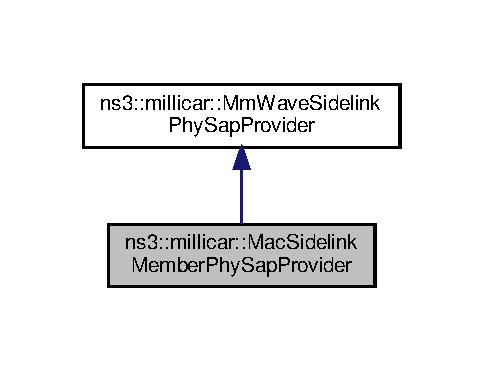
\includegraphics[width=232pt]{classns3_1_1millicar_1_1MacSidelinkMemberPhySapProvider__inherit__graph}
\end{center}
\end{figure}


Collaboration diagram for ns3\+:\+:millicar\+:\+:Mac\+Sidelink\+Member\+Phy\+Sap\+Provider\+:\nopagebreak
\begin{figure}[H]
\begin{center}
\leavevmode
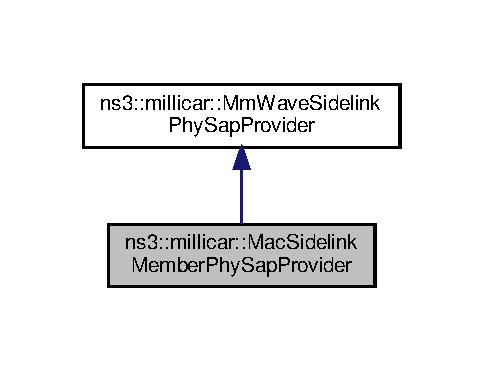
\includegraphics[width=232pt]{classns3_1_1millicar_1_1MacSidelinkMemberPhySapProvider__coll__graph}
\end{center}
\end{figure}
\subsection*{Public Member Functions}
\begin{DoxyCompactItemize}
\item 
\mbox{\Hypertarget{classns3_1_1millicar_1_1MacSidelinkMemberPhySapProvider_a82ef934739ad27061d4f59c15cdef118}\label{classns3_1_1millicar_1_1MacSidelinkMemberPhySapProvider_a82ef934739ad27061d4f59c15cdef118}} 
{\bfseries Mac\+Sidelink\+Member\+Phy\+Sap\+Provider} (Ptr$<$ \hyperlink{classns3_1_1millicar_1_1MmWaveSidelinkPhy}{Mm\+Wave\+Sidelink\+Phy} $>$ phy)
\item 
void \hyperlink{classns3_1_1millicar_1_1MacSidelinkMemberPhySapProvider_ad6a8a2b3021363432e870d4051448b15}{Add\+Transport\+Block} (Ptr$<$ Packet\+Burst $>$ pb, mmwave\+::\+Tti\+Alloc\+Info info) override
\begin{DoxyCompactList}\small\item\em Called by the upper layers to fill P\+HY\textquotesingle{}s buffer. \end{DoxyCompactList}\item 
void \hyperlink{classns3_1_1millicar_1_1MacSidelinkMemberPhySapProvider_afe0a87706052aabc88e7c4fbd4cc7a02}{Prepare\+For\+Reception} (uint16\+\_\+t rnti) override
\begin{DoxyCompactList}\small\item\em Called by the upper layer to prepare the P\+HY for the reception from another device. \end{DoxyCompactList}\end{DoxyCompactItemize}


\subsection{Member Function Documentation}
\mbox{\Hypertarget{classns3_1_1millicar_1_1MacSidelinkMemberPhySapProvider_ad6a8a2b3021363432e870d4051448b15}\label{classns3_1_1millicar_1_1MacSidelinkMemberPhySapProvider_ad6a8a2b3021363432e870d4051448b15}} 
\index{ns3\+::millicar\+::\+Mac\+Sidelink\+Member\+Phy\+Sap\+Provider@{ns3\+::millicar\+::\+Mac\+Sidelink\+Member\+Phy\+Sap\+Provider}!Add\+Transport\+Block@{Add\+Transport\+Block}}
\index{Add\+Transport\+Block@{Add\+Transport\+Block}!ns3\+::millicar\+::\+Mac\+Sidelink\+Member\+Phy\+Sap\+Provider@{ns3\+::millicar\+::\+Mac\+Sidelink\+Member\+Phy\+Sap\+Provider}}
\subsubsection{\texorpdfstring{Add\+Transport\+Block()}{AddTransportBlock()}}
{\footnotesize\ttfamily void ns3\+::millicar\+::\+Mac\+Sidelink\+Member\+Phy\+Sap\+Provider\+::\+Add\+Transport\+Block (\begin{DoxyParamCaption}\item[{Ptr$<$ Packet\+Burst $>$}]{pb,  }\item[{mmwave\+::\+Tti\+Alloc\+Info}]{info }\end{DoxyParamCaption})\hspace{0.3cm}{\ttfamily [override]}, {\ttfamily [virtual]}}



Called by the upper layers to fill P\+HY\textquotesingle{}s buffer. 


\begin{DoxyParams}{Parameters}
{\em pb} & burst of packets to be forwarded to the P\+HY layer \\
\hline
{\em info} & information about slot allocation necessary to determine the transmission parameters \\
\hline
\end{DoxyParams}


Implements \hyperlink{classns3_1_1millicar_1_1MmWaveSidelinkPhySapProvider_acba80cb123b9eb0fcacefde35a91909d}{ns3\+::millicar\+::\+Mm\+Wave\+Sidelink\+Phy\+Sap\+Provider}.

\mbox{\Hypertarget{classns3_1_1millicar_1_1MacSidelinkMemberPhySapProvider_afe0a87706052aabc88e7c4fbd4cc7a02}\label{classns3_1_1millicar_1_1MacSidelinkMemberPhySapProvider_afe0a87706052aabc88e7c4fbd4cc7a02}} 
\index{ns3\+::millicar\+::\+Mac\+Sidelink\+Member\+Phy\+Sap\+Provider@{ns3\+::millicar\+::\+Mac\+Sidelink\+Member\+Phy\+Sap\+Provider}!Prepare\+For\+Reception@{Prepare\+For\+Reception}}
\index{Prepare\+For\+Reception@{Prepare\+For\+Reception}!ns3\+::millicar\+::\+Mac\+Sidelink\+Member\+Phy\+Sap\+Provider@{ns3\+::millicar\+::\+Mac\+Sidelink\+Member\+Phy\+Sap\+Provider}}
\subsubsection{\texorpdfstring{Prepare\+For\+Reception()}{PrepareForReception()}}
{\footnotesize\ttfamily void ns3\+::millicar\+::\+Mac\+Sidelink\+Member\+Phy\+Sap\+Provider\+::\+Prepare\+For\+Reception (\begin{DoxyParamCaption}\item[{uint16\+\_\+t}]{rnti }\end{DoxyParamCaption})\hspace{0.3cm}{\ttfamily [override]}, {\ttfamily [virtual]}}



Called by the upper layer to prepare the P\+HY for the reception from another device. 


\begin{DoxyParams}{Parameters}
{\em rnti} & the rnti of the transmitting device \\
\hline
\end{DoxyParams}


Implements \hyperlink{classns3_1_1millicar_1_1MmWaveSidelinkPhySapProvider_a1c791fea7b4457a39428f3da49eaf6b8}{ns3\+::millicar\+::\+Mm\+Wave\+Sidelink\+Phy\+Sap\+Provider}.



The documentation for this class was generated from the following files\+:\begin{DoxyCompactItemize}
\item 
model/mmwave-\/sidelink-\/phy.\+h\item 
model/mmwave-\/sidelink-\/phy.\+cc\end{DoxyCompactItemize}

\hypertarget{classns3_1_1millicar_1_1MacSidelinkMemberPhySapUser}{}\section{ns3\+:\+:millicar\+:\+:Mac\+Sidelink\+Member\+Phy\+Sap\+User Class Reference}
\label{classns3_1_1millicar_1_1MacSidelinkMemberPhySapUser}\index{ns3\+::millicar\+::\+Mac\+Sidelink\+Member\+Phy\+Sap\+User@{ns3\+::millicar\+::\+Mac\+Sidelink\+Member\+Phy\+Sap\+User}}


Inheritance diagram for ns3\+:\+:millicar\+:\+:Mac\+Sidelink\+Member\+Phy\+Sap\+User\+:
\nopagebreak
\begin{figure}[H]
\begin{center}
\leavevmode
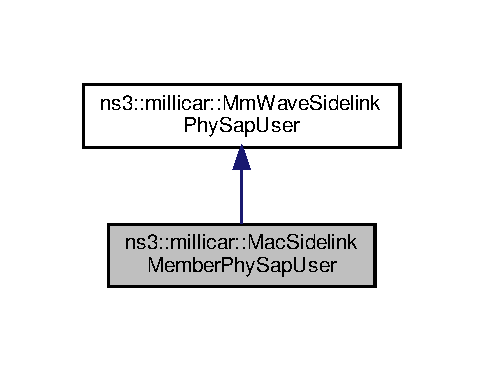
\includegraphics[width=232pt]{classns3_1_1millicar_1_1MacSidelinkMemberPhySapUser__inherit__graph}
\end{center}
\end{figure}


Collaboration diagram for ns3\+:\+:millicar\+:\+:Mac\+Sidelink\+Member\+Phy\+Sap\+User\+:
\nopagebreak
\begin{figure}[H]
\begin{center}
\leavevmode
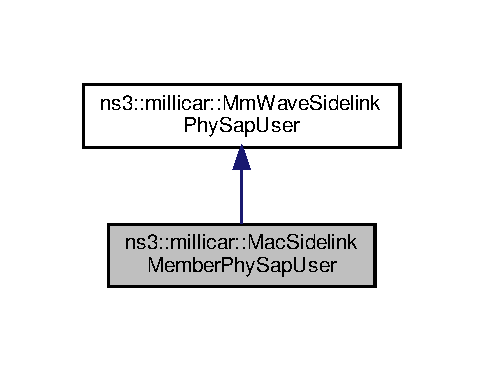
\includegraphics[width=232pt]{classns3_1_1millicar_1_1MacSidelinkMemberPhySapUser__coll__graph}
\end{center}
\end{figure}
\subsection*{Public Member Functions}
\begin{DoxyCompactItemize}
\item 
\mbox{\Hypertarget{classns3_1_1millicar_1_1MacSidelinkMemberPhySapUser_a52793da75596df4b84a8504274a6deb8}\label{classns3_1_1millicar_1_1MacSidelinkMemberPhySapUser_a52793da75596df4b84a8504274a6deb8}} 
{\bfseries Mac\+Sidelink\+Member\+Phy\+Sap\+User} (Ptr$<$ \hyperlink{classns3_1_1millicar_1_1MmWaveSidelinkMac}{Mm\+Wave\+Sidelink\+Mac} $>$ mac)
\item 
void \hyperlink{classns3_1_1millicar_1_1MacSidelinkMemberPhySapUser_a430a252dfedeea5228eab8e62af82960}{Receive\+Phy\+Pdu} (Ptr$<$ Packet $>$ p) override
\begin{DoxyCompactList}\small\item\em Called by the P\+HY to notify the M\+AC of the reception of a new P\+H\+Y-\/\+P\+DU. \end{DoxyCompactList}\item 
void \hyperlink{classns3_1_1millicar_1_1MacSidelinkMemberPhySapUser_ae204b07ff1b6fcd8d50dc71d21b51278}{Slot\+Indication} (mmwave\+::\+Sfn\+Sf timing\+Info) override
\begin{DoxyCompactList}\small\item\em Trigger the start from a new slot (input from P\+HY layer) \end{DoxyCompactList}\item 
void \hyperlink{classns3_1_1millicar_1_1MacSidelinkMemberPhySapUser_a68dd0cadd60b7bf0d2a3ac34a15a8e4c}{Sl\+Sinr\+Report} (const Spectrum\+Value \&sinr, uint16\+\_\+t rnti, uint8\+\_\+t num\+Sym, uint32\+\_\+t tb\+Size) override
\begin{DoxyCompactList}\small\item\em Reports the S\+I\+NR meausured with a certain device. \end{DoxyCompactList}\end{DoxyCompactItemize}


\subsection{Member Function Documentation}
\mbox{\Hypertarget{classns3_1_1millicar_1_1MacSidelinkMemberPhySapUser_a430a252dfedeea5228eab8e62af82960}\label{classns3_1_1millicar_1_1MacSidelinkMemberPhySapUser_a430a252dfedeea5228eab8e62af82960}} 
\index{ns3\+::millicar\+::\+Mac\+Sidelink\+Member\+Phy\+Sap\+User@{ns3\+::millicar\+::\+Mac\+Sidelink\+Member\+Phy\+Sap\+User}!Receive\+Phy\+Pdu@{Receive\+Phy\+Pdu}}
\index{Receive\+Phy\+Pdu@{Receive\+Phy\+Pdu}!ns3\+::millicar\+::\+Mac\+Sidelink\+Member\+Phy\+Sap\+User@{ns3\+::millicar\+::\+Mac\+Sidelink\+Member\+Phy\+Sap\+User}}
\subsubsection{\texorpdfstring{Receive\+Phy\+Pdu()}{ReceivePhyPdu()}}
{\footnotesize\ttfamily void ns3\+::millicar\+::\+Mac\+Sidelink\+Member\+Phy\+Sap\+User\+::\+Receive\+Phy\+Pdu (\begin{DoxyParamCaption}\item[{Ptr$<$ Packet $>$}]{p }\end{DoxyParamCaption})\hspace{0.3cm}{\ttfamily [override]}, {\ttfamily [virtual]}}



Called by the P\+HY to notify the M\+AC of the reception of a new P\+H\+Y-\/\+P\+DU. 


\begin{DoxyParams}{Parameters}
{\em p} & packet \\
\hline
\end{DoxyParams}


Implements \hyperlink{classns3_1_1millicar_1_1MmWaveSidelinkPhySapUser_ac0e4d40ace55e47cb3fb54d09c80fe06}{ns3\+::millicar\+::\+Mm\+Wave\+Sidelink\+Phy\+Sap\+User}.

\mbox{\Hypertarget{classns3_1_1millicar_1_1MacSidelinkMemberPhySapUser_ae204b07ff1b6fcd8d50dc71d21b51278}\label{classns3_1_1millicar_1_1MacSidelinkMemberPhySapUser_ae204b07ff1b6fcd8d50dc71d21b51278}} 
\index{ns3\+::millicar\+::\+Mac\+Sidelink\+Member\+Phy\+Sap\+User@{ns3\+::millicar\+::\+Mac\+Sidelink\+Member\+Phy\+Sap\+User}!Slot\+Indication@{Slot\+Indication}}
\index{Slot\+Indication@{Slot\+Indication}!ns3\+::millicar\+::\+Mac\+Sidelink\+Member\+Phy\+Sap\+User@{ns3\+::millicar\+::\+Mac\+Sidelink\+Member\+Phy\+Sap\+User}}
\subsubsection{\texorpdfstring{Slot\+Indication()}{SlotIndication()}}
{\footnotesize\ttfamily void ns3\+::millicar\+::\+Mac\+Sidelink\+Member\+Phy\+Sap\+User\+::\+Slot\+Indication (\begin{DoxyParamCaption}\item[{mmwave\+::\+Sfn\+Sf}]{timing\+Info }\end{DoxyParamCaption})\hspace{0.3cm}{\ttfamily [override]}, {\ttfamily [virtual]}}



Trigger the start from a new slot (input from P\+HY layer) 


\begin{DoxyParams}{Parameters}
{\em timing\+Info} & the structure containing the timing information \\
\hline
\end{DoxyParams}


Implements \hyperlink{classns3_1_1millicar_1_1MmWaveSidelinkPhySapUser_a237ec6c8c7496a3e021d22393ba7fc61}{ns3\+::millicar\+::\+Mm\+Wave\+Sidelink\+Phy\+Sap\+User}.

\mbox{\Hypertarget{classns3_1_1millicar_1_1MacSidelinkMemberPhySapUser_a68dd0cadd60b7bf0d2a3ac34a15a8e4c}\label{classns3_1_1millicar_1_1MacSidelinkMemberPhySapUser_a68dd0cadd60b7bf0d2a3ac34a15a8e4c}} 
\index{ns3\+::millicar\+::\+Mac\+Sidelink\+Member\+Phy\+Sap\+User@{ns3\+::millicar\+::\+Mac\+Sidelink\+Member\+Phy\+Sap\+User}!Sl\+Sinr\+Report@{Sl\+Sinr\+Report}}
\index{Sl\+Sinr\+Report@{Sl\+Sinr\+Report}!ns3\+::millicar\+::\+Mac\+Sidelink\+Member\+Phy\+Sap\+User@{ns3\+::millicar\+::\+Mac\+Sidelink\+Member\+Phy\+Sap\+User}}
\subsubsection{\texorpdfstring{Sl\+Sinr\+Report()}{SlSinrReport()}}
{\footnotesize\ttfamily void ns3\+::millicar\+::\+Mac\+Sidelink\+Member\+Phy\+Sap\+User\+::\+Sl\+Sinr\+Report (\begin{DoxyParamCaption}\item[{const Spectrum\+Value \&}]{sinr,  }\item[{uint16\+\_\+t}]{rnti,  }\item[{uint8\+\_\+t}]{num\+Sym,  }\item[{uint32\+\_\+t}]{tb\+Size }\end{DoxyParamCaption})\hspace{0.3cm}{\ttfamily [override]}, {\ttfamily [virtual]}}



Reports the S\+I\+NR meausured with a certain device. 


\begin{DoxyParams}{Parameters}
{\em sinr} & the S\+I\+NR \\
\hline
{\em rnti} & R\+N\+TI of the transmitting device \\
\hline
{\em num\+Sym} & size of the transport block that generated the report in number of O\+F\+DM symbols \\
\hline
{\em tb\+Size} & size of the transport block that generated the report in number of bytes \\
\hline
\end{DoxyParams}


Implements \hyperlink{classns3_1_1millicar_1_1MmWaveSidelinkPhySapUser_aedb96411ce5a46589df517b1aa272d97}{ns3\+::millicar\+::\+Mm\+Wave\+Sidelink\+Phy\+Sap\+User}.



The documentation for this class was generated from the following files\+:\begin{DoxyCompactItemize}
\item 
model/mmwave-\/sidelink-\/mac.\+h\item 
model/mmwave-\/sidelink-\/mac.\+cc\end{DoxyCompactItemize}

\hypertarget{classns3_1_1millicar_1_1MmWaveSidelinkMac}{}\section{ns3\+:\+:millicar\+:\+:Mm\+Wave\+Sidelink\+Mac Class Reference}
\label{classns3_1_1millicar_1_1MmWaveSidelinkMac}\index{ns3\+::millicar\+::\+Mm\+Wave\+Sidelink\+Mac@{ns3\+::millicar\+::\+Mm\+Wave\+Sidelink\+Mac}}


Inheritance diagram for ns3\+:\+:millicar\+:\+:Mm\+Wave\+Sidelink\+Mac\+:\nopagebreak
\begin{figure}[H]
\begin{center}
\leavevmode
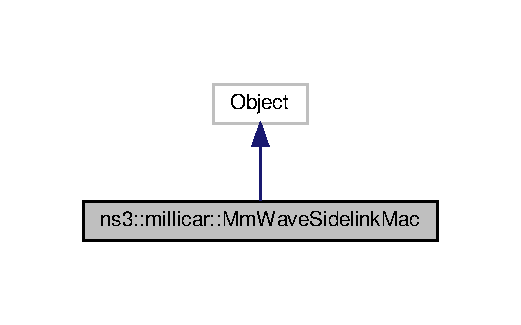
\includegraphics[width=250pt]{classns3_1_1millicar_1_1MmWaveSidelinkMac__inherit__graph}
\end{center}
\end{figure}


Collaboration diagram for ns3\+:\+:millicar\+:\+:Mm\+Wave\+Sidelink\+Mac\+:\nopagebreak
\begin{figure}[H]
\begin{center}
\leavevmode
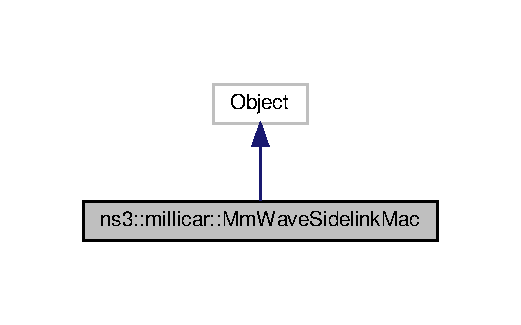
\includegraphics[width=250pt]{classns3_1_1millicar_1_1MmWaveSidelinkMac__coll__graph}
\end{center}
\end{figure}
\subsection*{Public Types}
\begin{DoxyCompactItemize}
\item 
typedef void($\ast$ \hyperlink{classns3_1_1millicar_1_1MmWaveSidelinkMac_ad5c7416a57edcebe1e57106b503831c7}{Sl\+Scheduling\+Traced\+Callback}) (\hyperlink{structns3_1_1millicar_1_1SlSchedulingCallback}{Sl\+Scheduling\+Callback} params)
\end{DoxyCompactItemize}
\subsection*{Public Member Functions}
\begin{DoxyCompactItemize}
\item 
\mbox{\Hypertarget{classns3_1_1millicar_1_1MmWaveSidelinkMac_a2c96de8928cbba2b7c8b0f71f2318e54}\label{classns3_1_1millicar_1_1MmWaveSidelinkMac_a2c96de8928cbba2b7c8b0f71f2318e54}} 
\hyperlink{classns3_1_1millicar_1_1MmWaveSidelinkMac_a2c96de8928cbba2b7c8b0f71f2318e54}{Mm\+Wave\+Sidelink\+Mac} (void)=delete
\begin{DoxyCompactList}\small\item\em Delete default constructor to avoid misuse. \end{DoxyCompactList}\item 
\hyperlink{classns3_1_1millicar_1_1MmWaveSidelinkMac_ae4a82035baa66ee6c17d9b2094bacd24}{Mm\+Wave\+Sidelink\+Mac} (Ptr$<$ mmwave\+::\+Mm\+Wave\+Phy\+Mac\+Common $>$ pmc)
\begin{DoxyCompactList}\small\item\em Class constructor. \end{DoxyCompactList}\item 
\mbox{\Hypertarget{classns3_1_1millicar_1_1MmWaveSidelinkMac_a8a34b3d135b391d9fc16004fb91fa208}\label{classns3_1_1millicar_1_1MmWaveSidelinkMac_a8a34b3d135b391d9fc16004fb91fa208}} 
\hyperlink{classns3_1_1millicar_1_1MmWaveSidelinkMac_a8a34b3d135b391d9fc16004fb91fa208}{$\sim$\+Mm\+Wave\+Sidelink\+Mac} (void)
\begin{DoxyCompactList}\small\item\em Class destructor. \end{DoxyCompactList}\item 
\mbox{\Hypertarget{classns3_1_1millicar_1_1MmWaveSidelinkMac_af5aee81d76bc85ab6d57742cffc214de}\label{classns3_1_1millicar_1_1MmWaveSidelinkMac_af5aee81d76bc85ab6d57742cffc214de}} 
virtual void \hyperlink{classns3_1_1millicar_1_1MmWaveSidelinkMac_af5aee81d76bc85ab6d57742cffc214de}{Do\+Dispose} (void)
\begin{DoxyCompactList}\small\item\em Destructor implementation. \end{DoxyCompactList}\item 
void \hyperlink{classns3_1_1millicar_1_1MmWaveSidelinkMac_af1c118a5b92dfce7a7b62c55ac50c020}{Do\+Slot\+Indication} (mmwave\+::\+Sfn\+Sf timing\+Info)
\begin{DoxyCompactList}\small\item\em trigger the start of a new slot with all the necessary information \end{DoxyCompactList}\item 
\hyperlink{classns3_1_1millicar_1_1MmWaveSidelinkPhySapUser}{Mm\+Wave\+Sidelink\+Phy\+Sap\+User} $\ast$ \hyperlink{classns3_1_1millicar_1_1MmWaveSidelinkMac_ae6a8f2b11ed7ac5d33dc0629937695e6}{Get\+Phy\+Sap\+User} () const
\begin{DoxyCompactList}\small\item\em Get the P\+HY S\+AP user. \end{DoxyCompactList}\item 
void \hyperlink{classns3_1_1millicar_1_1MmWaveSidelinkMac_a42acefcfc918c3500669e32e40bf42a0}{Set\+Phy\+Sap\+Provider} (\hyperlink{classns3_1_1millicar_1_1MmWaveSidelinkPhySapProvider}{Mm\+Wave\+Sidelink\+Phy\+Sap\+Provider} $\ast$sap)
\begin{DoxyCompactList}\small\item\em Set the P\+HY S\+AP provider. \end{DoxyCompactList}\item 
Lte\+Mac\+Sap\+Provider $\ast$ \hyperlink{classns3_1_1millicar_1_1MmWaveSidelinkMac_a9ac166a4e4d5e2449cb0e69a165719cb}{Get\+Mac\+Sap\+Provider} () const
\begin{DoxyCompactList}\small\item\em return the M\+AC S\+AP provider \end{DoxyCompactList}\item 
void \hyperlink{classns3_1_1millicar_1_1MmWaveSidelinkMac_af1686c0688c1bafeccb463ea2bc6f828}{Set\+Rnti} (uint16\+\_\+t rnti)
\begin{DoxyCompactList}\small\item\em assign a proper value to the R\+N\+TI associated to a specific user \end{DoxyCompactList}\item 
uint16\+\_\+t \hyperlink{classns3_1_1millicar_1_1MmWaveSidelinkMac_a229809ca241dc9416dfb8ec82d8e48f6}{Get\+Rnti} () const
\begin{DoxyCompactList}\small\item\em return the R\+N\+TI associated to a specific user \end{DoxyCompactList}\item 
void \hyperlink{classns3_1_1millicar_1_1MmWaveSidelinkMac_a3862171847195f4cf9122fb8f05ed3eb}{Set\+Sf\+Allocation\+Info} (std\+::vector$<$ uint16\+\_\+t $>$ pattern)
\begin{DoxyCompactList}\small\item\em set the subframe allocation pattern \end{DoxyCompactList}\item 
\mbox{\Hypertarget{classns3_1_1millicar_1_1MmWaveSidelinkMac_a36bc120898406b4fa124ec340266e30a}\label{classns3_1_1millicar_1_1MmWaveSidelinkMac_a36bc120898406b4fa124ec340266e30a}} 
void \hyperlink{classns3_1_1millicar_1_1MmWaveSidelinkMac_a36bc120898406b4fa124ec340266e30a}{Do\+Transmit\+Pdu} (Lte\+Mac\+Sap\+Provider\+::\+Transmit\+Pdu\+Parameters params)
\begin{DoxyCompactList}\small\item\em Transmit P\+DU function. \end{DoxyCompactList}\item 
void \hyperlink{classns3_1_1millicar_1_1MmWaveSidelinkMac_af303cc45866c7094f9f2c36bbaa0a66c}{Set\+Forward\+Up\+Callback} (Callback$<$ void, Ptr$<$ Packet $>$ $>$ cb)
\begin{DoxyCompactList}\small\item\em set the callback used to forward data packets up to the Net\+Device \end{DoxyCompactList}\item 
void \hyperlink{classns3_1_1millicar_1_1MmWaveSidelinkMac_ad4c32a42bd58226a3ad07828e7b4cff0}{Add\+Mac\+Sap\+User} (uint8\+\_\+t lcid, Lte\+Mac\+Sap\+User $\ast$mac\+Sap\+User)
\end{DoxyCompactItemize}
\subsection*{Static Public Member Functions}
\begin{DoxyCompactItemize}
\item 
static Type\+Id \hyperlink{classns3_1_1millicar_1_1MmWaveSidelinkMac_a97fdea26e60baec2ab5f082da054e18e}{Get\+Type\+Id} (void)
\begin{DoxyCompactList}\small\item\em Get the type ID. \end{DoxyCompactList}\end{DoxyCompactItemize}
\subsection*{Friends}
\begin{DoxyCompactItemize}
\item 
\mbox{\Hypertarget{classns3_1_1millicar_1_1MmWaveSidelinkMac_a7718a67d36cf06d1d96b26fbea6910eb}\label{classns3_1_1millicar_1_1MmWaveSidelinkMac_a7718a67d36cf06d1d96b26fbea6910eb}} 
class {\bfseries Mac\+Sidelink\+Member\+Phy\+Sap\+User}
\item 
\mbox{\Hypertarget{classns3_1_1millicar_1_1MmWaveSidelinkMac_a60d31e68fce742d4da754d8f69824337}\label{classns3_1_1millicar_1_1MmWaveSidelinkMac_a60d31e68fce742d4da754d8f69824337}} 
class {\bfseries Rlc\+Sidelink\+Member\+Mac\+Sap\+Provider}
\end{DoxyCompactItemize}


\subsection{Member Typedef Documentation}
\mbox{\Hypertarget{classns3_1_1millicar_1_1MmWaveSidelinkMac_ad5c7416a57edcebe1e57106b503831c7}\label{classns3_1_1millicar_1_1MmWaveSidelinkMac_ad5c7416a57edcebe1e57106b503831c7}} 
\index{ns3\+::millicar\+::\+Mm\+Wave\+Sidelink\+Mac@{ns3\+::millicar\+::\+Mm\+Wave\+Sidelink\+Mac}!Sl\+Scheduling\+Traced\+Callback@{Sl\+Scheduling\+Traced\+Callback}}
\index{Sl\+Scheduling\+Traced\+Callback@{Sl\+Scheduling\+Traced\+Callback}!ns3\+::millicar\+::\+Mm\+Wave\+Sidelink\+Mac@{ns3\+::millicar\+::\+Mm\+Wave\+Sidelink\+Mac}}
\subsubsection{\texorpdfstring{Sl\+Scheduling\+Traced\+Callback}{SlSchedulingTracedCallback}}
{\footnotesize\ttfamily typedef void($\ast$  ns3\+::millicar\+::\+Mm\+Wave\+Sidelink\+Mac\+::\+Sl\+Scheduling\+Traced\+Callback) (\hyperlink{structns3_1_1millicar_1_1SlSchedulingCallback}{Sl\+Scheduling\+Callback} params)}

Traced\+Callback signature for SL scheduling


\begin{DoxyParams}{Parameters}
{\em params} & the struct \hyperlink{structns3_1_1millicar_1_1SlSchedulingCallback}{Sl\+Scheduling\+Callback} containing the scheduling info \\
\hline
\end{DoxyParams}


\subsection{Constructor \& Destructor Documentation}
\mbox{\Hypertarget{classns3_1_1millicar_1_1MmWaveSidelinkMac_ae4a82035baa66ee6c17d9b2094bacd24}\label{classns3_1_1millicar_1_1MmWaveSidelinkMac_ae4a82035baa66ee6c17d9b2094bacd24}} 
\index{ns3\+::millicar\+::\+Mm\+Wave\+Sidelink\+Mac@{ns3\+::millicar\+::\+Mm\+Wave\+Sidelink\+Mac}!Mm\+Wave\+Sidelink\+Mac@{Mm\+Wave\+Sidelink\+Mac}}
\index{Mm\+Wave\+Sidelink\+Mac@{Mm\+Wave\+Sidelink\+Mac}!ns3\+::millicar\+::\+Mm\+Wave\+Sidelink\+Mac@{ns3\+::millicar\+::\+Mm\+Wave\+Sidelink\+Mac}}
\subsubsection{\texorpdfstring{Mm\+Wave\+Sidelink\+Mac()}{MmWaveSidelinkMac()}}
{\footnotesize\ttfamily ns3\+::millicar\+::\+Mm\+Wave\+Sidelink\+Mac\+::\+Mm\+Wave\+Sidelink\+Mac (\begin{DoxyParamCaption}\item[{Ptr$<$ mmwave\+::\+Mm\+Wave\+Phy\+Mac\+Common $>$}]{pmc }\end{DoxyParamCaption})}



Class constructor. 


\begin{DoxyParams}{Parameters}
{\em pmc} & pointer to the mmwave\+::\+Mm\+Wave\+Phy\+Mac\+Common instance which specifies the P\+H\+Y/\+M\+AC parameters \\
\hline
\end{DoxyParams}


\subsection{Member Function Documentation}
\mbox{\Hypertarget{classns3_1_1millicar_1_1MmWaveSidelinkMac_ad4c32a42bd58226a3ad07828e7b4cff0}\label{classns3_1_1millicar_1_1MmWaveSidelinkMac_ad4c32a42bd58226a3ad07828e7b4cff0}} 
\index{ns3\+::millicar\+::\+Mm\+Wave\+Sidelink\+Mac@{ns3\+::millicar\+::\+Mm\+Wave\+Sidelink\+Mac}!Add\+Mac\+Sap\+User@{Add\+Mac\+Sap\+User}}
\index{Add\+Mac\+Sap\+User@{Add\+Mac\+Sap\+User}!ns3\+::millicar\+::\+Mm\+Wave\+Sidelink\+Mac@{ns3\+::millicar\+::\+Mm\+Wave\+Sidelink\+Mac}}
\subsubsection{\texorpdfstring{Add\+Mac\+Sap\+User()}{AddMacSapUser()}}
{\footnotesize\ttfamily void ns3\+::millicar\+::\+Mm\+Wave\+Sidelink\+Mac\+::\+Add\+Mac\+Sap\+User (\begin{DoxyParamCaption}\item[{uint8\+\_\+t}]{lcid,  }\item[{Lte\+Mac\+Sap\+User $\ast$}]{mac\+Sap\+User }\end{DoxyParamCaption})}

Associate a M\+AC S\+AP user instance to the L\+C\+ID and add it in the map 
\begin{DoxyParams}{Parameters}
{\em lcid} & Logical Channel ID \\
\hline
{\em mac\+Sap\+User} & Lte\+Mac\+Sap\+User to be associated to a single L\+C\+ID and added to the respective map \\
\hline
\end{DoxyParams}
\mbox{\Hypertarget{classns3_1_1millicar_1_1MmWaveSidelinkMac_af1c118a5b92dfce7a7b62c55ac50c020}\label{classns3_1_1millicar_1_1MmWaveSidelinkMac_af1c118a5b92dfce7a7b62c55ac50c020}} 
\index{ns3\+::millicar\+::\+Mm\+Wave\+Sidelink\+Mac@{ns3\+::millicar\+::\+Mm\+Wave\+Sidelink\+Mac}!Do\+Slot\+Indication@{Do\+Slot\+Indication}}
\index{Do\+Slot\+Indication@{Do\+Slot\+Indication}!ns3\+::millicar\+::\+Mm\+Wave\+Sidelink\+Mac@{ns3\+::millicar\+::\+Mm\+Wave\+Sidelink\+Mac}}
\subsubsection{\texorpdfstring{Do\+Slot\+Indication()}{DoSlotIndication()}}
{\footnotesize\ttfamily void ns3\+::millicar\+::\+Mm\+Wave\+Sidelink\+Mac\+::\+Do\+Slot\+Indication (\begin{DoxyParamCaption}\item[{mmwave\+::\+Sfn\+Sf}]{timing\+Info }\end{DoxyParamCaption})}



trigger the start of a new slot with all the necessary information 


\begin{DoxyParams}{Parameters}
{\em timing\+Info} & the structure containing the timing information \\
\hline
\end{DoxyParams}
\mbox{\Hypertarget{classns3_1_1millicar_1_1MmWaveSidelinkMac_a9ac166a4e4d5e2449cb0e69a165719cb}\label{classns3_1_1millicar_1_1MmWaveSidelinkMac_a9ac166a4e4d5e2449cb0e69a165719cb}} 
\index{ns3\+::millicar\+::\+Mm\+Wave\+Sidelink\+Mac@{ns3\+::millicar\+::\+Mm\+Wave\+Sidelink\+Mac}!Get\+Mac\+Sap\+Provider@{Get\+Mac\+Sap\+Provider}}
\index{Get\+Mac\+Sap\+Provider@{Get\+Mac\+Sap\+Provider}!ns3\+::millicar\+::\+Mm\+Wave\+Sidelink\+Mac@{ns3\+::millicar\+::\+Mm\+Wave\+Sidelink\+Mac}}
\subsubsection{\texorpdfstring{Get\+Mac\+Sap\+Provider()}{GetMacSapProvider()}}
{\footnotesize\ttfamily Lte\+Mac\+Sap\+Provider $\ast$ ns3\+::millicar\+::\+Mm\+Wave\+Sidelink\+Mac\+::\+Get\+Mac\+Sap\+Provider (\begin{DoxyParamCaption}{ }\end{DoxyParamCaption}) const}



return the M\+AC S\+AP provider 

\begin{DoxyReturn}{Returns}
the Mac\+Sap\+Provider 
\end{DoxyReturn}
\mbox{\Hypertarget{classns3_1_1millicar_1_1MmWaveSidelinkMac_ae6a8f2b11ed7ac5d33dc0629937695e6}\label{classns3_1_1millicar_1_1MmWaveSidelinkMac_ae6a8f2b11ed7ac5d33dc0629937695e6}} 
\index{ns3\+::millicar\+::\+Mm\+Wave\+Sidelink\+Mac@{ns3\+::millicar\+::\+Mm\+Wave\+Sidelink\+Mac}!Get\+Phy\+Sap\+User@{Get\+Phy\+Sap\+User}}
\index{Get\+Phy\+Sap\+User@{Get\+Phy\+Sap\+User}!ns3\+::millicar\+::\+Mm\+Wave\+Sidelink\+Mac@{ns3\+::millicar\+::\+Mm\+Wave\+Sidelink\+Mac}}
\subsubsection{\texorpdfstring{Get\+Phy\+Sap\+User()}{GetPhySapUser()}}
{\footnotesize\ttfamily \hyperlink{classns3_1_1millicar_1_1MmWaveSidelinkPhySapUser}{Mm\+Wave\+Sidelink\+Phy\+Sap\+User} $\ast$ ns3\+::millicar\+::\+Mm\+Wave\+Sidelink\+Mac\+::\+Get\+Phy\+Sap\+User (\begin{DoxyParamCaption}{ }\end{DoxyParamCaption}) const}



Get the P\+HY S\+AP user. 

\begin{DoxyReturn}{Returns}
a pointer to the S\+AP user 
\end{DoxyReturn}
\mbox{\Hypertarget{classns3_1_1millicar_1_1MmWaveSidelinkMac_a229809ca241dc9416dfb8ec82d8e48f6}\label{classns3_1_1millicar_1_1MmWaveSidelinkMac_a229809ca241dc9416dfb8ec82d8e48f6}} 
\index{ns3\+::millicar\+::\+Mm\+Wave\+Sidelink\+Mac@{ns3\+::millicar\+::\+Mm\+Wave\+Sidelink\+Mac}!Get\+Rnti@{Get\+Rnti}}
\index{Get\+Rnti@{Get\+Rnti}!ns3\+::millicar\+::\+Mm\+Wave\+Sidelink\+Mac@{ns3\+::millicar\+::\+Mm\+Wave\+Sidelink\+Mac}}
\subsubsection{\texorpdfstring{Get\+Rnti()}{GetRnti()}}
{\footnotesize\ttfamily uint16\+\_\+t ns3\+::millicar\+::\+Mm\+Wave\+Sidelink\+Mac\+::\+Get\+Rnti (\begin{DoxyParamCaption}{ }\end{DoxyParamCaption}) const}



return the R\+N\+TI associated to a specific user 

\begin{DoxyReturn}{Returns}
the R\+N\+TI 
\end{DoxyReturn}
\mbox{\Hypertarget{classns3_1_1millicar_1_1MmWaveSidelinkMac_a97fdea26e60baec2ab5f082da054e18e}\label{classns3_1_1millicar_1_1MmWaveSidelinkMac_a97fdea26e60baec2ab5f082da054e18e}} 
\index{ns3\+::millicar\+::\+Mm\+Wave\+Sidelink\+Mac@{ns3\+::millicar\+::\+Mm\+Wave\+Sidelink\+Mac}!Get\+Type\+Id@{Get\+Type\+Id}}
\index{Get\+Type\+Id@{Get\+Type\+Id}!ns3\+::millicar\+::\+Mm\+Wave\+Sidelink\+Mac@{ns3\+::millicar\+::\+Mm\+Wave\+Sidelink\+Mac}}
\subsubsection{\texorpdfstring{Get\+Type\+Id()}{GetTypeId()}}
{\footnotesize\ttfamily Type\+Id ns3\+::millicar\+::\+Mm\+Wave\+Sidelink\+Mac\+::\+Get\+Type\+Id (\begin{DoxyParamCaption}\item[{void}]{ }\end{DoxyParamCaption})\hspace{0.3cm}{\ttfamily [static]}}



Get the type ID. 

\begin{DoxyReturn}{Returns}
the object Type\+Id 
\end{DoxyReturn}
\mbox{\Hypertarget{classns3_1_1millicar_1_1MmWaveSidelinkMac_af303cc45866c7094f9f2c36bbaa0a66c}\label{classns3_1_1millicar_1_1MmWaveSidelinkMac_af303cc45866c7094f9f2c36bbaa0a66c}} 
\index{ns3\+::millicar\+::\+Mm\+Wave\+Sidelink\+Mac@{ns3\+::millicar\+::\+Mm\+Wave\+Sidelink\+Mac}!Set\+Forward\+Up\+Callback@{Set\+Forward\+Up\+Callback}}
\index{Set\+Forward\+Up\+Callback@{Set\+Forward\+Up\+Callback}!ns3\+::millicar\+::\+Mm\+Wave\+Sidelink\+Mac@{ns3\+::millicar\+::\+Mm\+Wave\+Sidelink\+Mac}}
\subsubsection{\texorpdfstring{Set\+Forward\+Up\+Callback()}{SetForwardUpCallback()}}
{\footnotesize\ttfamily void ns3\+::millicar\+::\+Mm\+Wave\+Sidelink\+Mac\+::\+Set\+Forward\+Up\+Callback (\begin{DoxyParamCaption}\item[{Callback$<$ void, Ptr$<$ Packet $>$ $>$}]{cb }\end{DoxyParamCaption})}



set the callback used to forward data packets up to the Net\+Device 


\begin{DoxyParams}{Parameters}
{\em cb} & the callback \\
\hline
\end{DoxyParams}
\mbox{\Hypertarget{classns3_1_1millicar_1_1MmWaveSidelinkMac_a42acefcfc918c3500669e32e40bf42a0}\label{classns3_1_1millicar_1_1MmWaveSidelinkMac_a42acefcfc918c3500669e32e40bf42a0}} 
\index{ns3\+::millicar\+::\+Mm\+Wave\+Sidelink\+Mac@{ns3\+::millicar\+::\+Mm\+Wave\+Sidelink\+Mac}!Set\+Phy\+Sap\+Provider@{Set\+Phy\+Sap\+Provider}}
\index{Set\+Phy\+Sap\+Provider@{Set\+Phy\+Sap\+Provider}!ns3\+::millicar\+::\+Mm\+Wave\+Sidelink\+Mac@{ns3\+::millicar\+::\+Mm\+Wave\+Sidelink\+Mac}}
\subsubsection{\texorpdfstring{Set\+Phy\+Sap\+Provider()}{SetPhySapProvider()}}
{\footnotesize\ttfamily void ns3\+::millicar\+::\+Mm\+Wave\+Sidelink\+Mac\+::\+Set\+Phy\+Sap\+Provider (\begin{DoxyParamCaption}\item[{\hyperlink{classns3_1_1millicar_1_1MmWaveSidelinkPhySapProvider}{Mm\+Wave\+Sidelink\+Phy\+Sap\+Provider} $\ast$}]{sap }\end{DoxyParamCaption})}



Set the P\+HY S\+AP provider. 


\begin{DoxyParams}{Parameters}
{\em sap} & the P\+HY S\+AP provider \\
\hline
\end{DoxyParams}
\mbox{\Hypertarget{classns3_1_1millicar_1_1MmWaveSidelinkMac_af1686c0688c1bafeccb463ea2bc6f828}\label{classns3_1_1millicar_1_1MmWaveSidelinkMac_af1686c0688c1bafeccb463ea2bc6f828}} 
\index{ns3\+::millicar\+::\+Mm\+Wave\+Sidelink\+Mac@{ns3\+::millicar\+::\+Mm\+Wave\+Sidelink\+Mac}!Set\+Rnti@{Set\+Rnti}}
\index{Set\+Rnti@{Set\+Rnti}!ns3\+::millicar\+::\+Mm\+Wave\+Sidelink\+Mac@{ns3\+::millicar\+::\+Mm\+Wave\+Sidelink\+Mac}}
\subsubsection{\texorpdfstring{Set\+Rnti()}{SetRnti()}}
{\footnotesize\ttfamily void ns3\+::millicar\+::\+Mm\+Wave\+Sidelink\+Mac\+::\+Set\+Rnti (\begin{DoxyParamCaption}\item[{uint16\+\_\+t}]{rnti }\end{DoxyParamCaption})}



assign a proper value to the R\+N\+TI associated to a specific user 


\begin{DoxyParams}{Parameters}
{\em rnti} & value of the rnti \\
\hline
\end{DoxyParams}
\mbox{\Hypertarget{classns3_1_1millicar_1_1MmWaveSidelinkMac_a3862171847195f4cf9122fb8f05ed3eb}\label{classns3_1_1millicar_1_1MmWaveSidelinkMac_a3862171847195f4cf9122fb8f05ed3eb}} 
\index{ns3\+::millicar\+::\+Mm\+Wave\+Sidelink\+Mac@{ns3\+::millicar\+::\+Mm\+Wave\+Sidelink\+Mac}!Set\+Sf\+Allocation\+Info@{Set\+Sf\+Allocation\+Info}}
\index{Set\+Sf\+Allocation\+Info@{Set\+Sf\+Allocation\+Info}!ns3\+::millicar\+::\+Mm\+Wave\+Sidelink\+Mac@{ns3\+::millicar\+::\+Mm\+Wave\+Sidelink\+Mac}}
\subsubsection{\texorpdfstring{Set\+Sf\+Allocation\+Info()}{SetSfAllocationInfo()}}
{\footnotesize\ttfamily void ns3\+::millicar\+::\+Mm\+Wave\+Sidelink\+Mac\+::\+Set\+Sf\+Allocation\+Info (\begin{DoxyParamCaption}\item[{std\+::vector$<$ uint16\+\_\+t $>$}]{pattern }\end{DoxyParamCaption})}



set the subframe allocation pattern 


\begin{DoxyParams}{Parameters}
{\em pattern} & the allocation pattern. The number of element must be equal to number of slots per subframe. Each element represents the R\+N\+TI of the device scheduled in the corresponding slot. \\
\hline
\end{DoxyParams}


The documentation for this class was generated from the following files\+:\begin{DoxyCompactItemize}
\item 
model/mmwave-\/sidelink-\/mac.\+h\item 
model/mmwave-\/sidelink-\/mac.\+cc\end{DoxyCompactItemize}

\hypertarget{classns3_1_1millicar_1_1MmWaveSidelinkPhy}{}\section{ns3\+:\+:millicar\+:\+:Mm\+Wave\+Sidelink\+Phy Class Reference}
\label{classns3_1_1millicar_1_1MmWaveSidelinkPhy}\index{ns3\+::millicar\+::\+Mm\+Wave\+Sidelink\+Phy@{ns3\+::millicar\+::\+Mm\+Wave\+Sidelink\+Phy}}


Inheritance diagram for ns3\+:\+:millicar\+:\+:Mm\+Wave\+Sidelink\+Phy\+:
\nopagebreak
\begin{figure}[H]
\begin{center}
\leavevmode
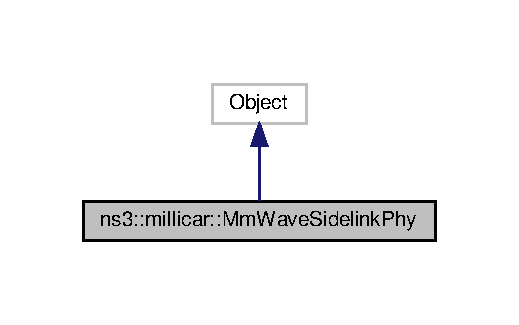
\includegraphics[width=249pt]{classns3_1_1millicar_1_1MmWaveSidelinkPhy__inherit__graph}
\end{center}
\end{figure}


Collaboration diagram for ns3\+:\+:millicar\+:\+:Mm\+Wave\+Sidelink\+Phy\+:
\nopagebreak
\begin{figure}[H]
\begin{center}
\leavevmode
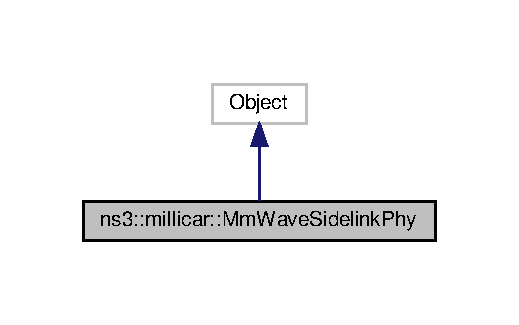
\includegraphics[width=249pt]{classns3_1_1millicar_1_1MmWaveSidelinkPhy__coll__graph}
\end{center}
\end{figure}
\subsection*{Public Member Functions}
\begin{DoxyCompactItemize}
\item 
\hyperlink{classns3_1_1millicar_1_1MmWaveSidelinkPhy_a6e37d7c3454a97b25e058a0bc4dd7bb6}{Mm\+Wave\+Sidelink\+Phy} ()
\item 
\hyperlink{classns3_1_1millicar_1_1MmWaveSidelinkPhy_ad8eab5190cd17e75f8d3e8711f16b76e}{Mm\+Wave\+Sidelink\+Phy} (Ptr$<$ \hyperlink{classns3_1_1millicar_1_1MmWaveSidelinkSpectrumPhy}{Mm\+Wave\+Sidelink\+Spectrum\+Phy} $>$ spectrum\+Phy, Ptr$<$ mmwave\+::\+Mm\+Wave\+Phy\+Mac\+Common $>$ conf\+Params)
\item 
virtual \hyperlink{classns3_1_1millicar_1_1MmWaveSidelinkPhy_ab0a97172cbc36ed6d0357761ca06af92}{$\sim$\+Mm\+Wave\+Sidelink\+Phy} ()
\item 
\mbox{\Hypertarget{classns3_1_1millicar_1_1MmWaveSidelinkPhy_a892c42e5b40f18979e0ebd01953bae7a}\label{classns3_1_1millicar_1_1MmWaveSidelinkPhy_a892c42e5b40f18979e0ebd01953bae7a}} 
virtual void {\bfseries Do\+Initialize} (void)
\item 
\mbox{\Hypertarget{classns3_1_1millicar_1_1MmWaveSidelinkPhy_a0a4c5d35850f4ee0d23a626f41652441}\label{classns3_1_1millicar_1_1MmWaveSidelinkPhy_a0a4c5d35850f4ee0d23a626f41652441}} 
virtual void {\bfseries Do\+Dispose} (void)
\item 
void \hyperlink{classns3_1_1millicar_1_1MmWaveSidelinkPhy_a58cf1b6bffacbf29abec6feb0cb35253}{Set\+Tx\+Power} (double power)
\item 
double \hyperlink{classns3_1_1millicar_1_1MmWaveSidelinkPhy_ae1c99f95c48cbdaf4066f1a4310ffff2}{Get\+Tx\+Power} () const
\item 
void \hyperlink{classns3_1_1millicar_1_1MmWaveSidelinkPhy_a3003041c8b2124b9c527b0bfe516c9ee}{Set\+Noise\+Figure} (double pf)
\item 
double \hyperlink{classns3_1_1millicar_1_1MmWaveSidelinkPhy_adcc119b8134bc2ee18088a0ef7c298e3}{Get\+Noise\+Figure} () const
\item 
Ptr$<$ mmwave\+::\+Mm\+Wave\+Phy\+Mac\+Common $>$ \hyperlink{classns3_1_1millicar_1_1MmWaveSidelinkPhy_aa774d38f7f3597cf79b2d55f16a1d2ba}{Get\+Configuration\+Parameters} (void) const
\item 
Ptr$<$ \hyperlink{classns3_1_1millicar_1_1MmWaveSidelinkSpectrumPhy}{Mm\+Wave\+Sidelink\+Spectrum\+Phy} $>$ \hyperlink{classns3_1_1millicar_1_1MmWaveSidelinkPhy_ad351ad92c46d2250c1848cc6f45d3de9}{Get\+Spectrum\+Phy} () const
\item 
\hyperlink{classns3_1_1millicar_1_1MmWaveSidelinkPhySapProvider}{Mm\+Wave\+Sidelink\+Phy\+Sap\+Provider} $\ast$ \hyperlink{classns3_1_1millicar_1_1MmWaveSidelinkPhy_ab8df82d08b89cfa181a548ca935409bf}{Get\+Phy\+Sap\+Provider} () const
\item 
void \hyperlink{classns3_1_1millicar_1_1MmWaveSidelinkPhy_af8a8ca9aa014acc288b7f36e549c56f7}{Set\+Phy\+Sap\+User} (\hyperlink{classns3_1_1millicar_1_1MmWaveSidelinkPhySapUser}{Mm\+Wave\+Sidelink\+Phy\+Sap\+User} $\ast$sap)
\item 
void \hyperlink{classns3_1_1millicar_1_1MmWaveSidelinkPhy_a8dbf76a5946b77c520dbcc2313c32bf6}{Add\+Device} (uint64\+\_\+t rnti, Ptr$<$ Net\+Device $>$ dev)
\item 
void \hyperlink{classns3_1_1millicar_1_1MmWaveSidelinkPhy_a9a6b48f434ad30b0c61d246c6a98c766}{Do\+Add\+Transport\+Block} (Ptr$<$ Packet\+Burst $>$ pb, mmwave\+::\+Tti\+Alloc\+Info info)
\item 
void \hyperlink{classns3_1_1millicar_1_1MmWaveSidelinkPhy_a8b5f228e68d5f66539d99bada58eff17}{Do\+Prepare\+For\+Reception\+From} (uint16\+\_\+t rnti)
\item 
void \hyperlink{classns3_1_1millicar_1_1MmWaveSidelinkPhy_a5721f99acca7de2ee5c9ae8e926eb48a}{Receive} (Ptr$<$ Packet $>$ p)
\item 
void \hyperlink{classns3_1_1millicar_1_1MmWaveSidelinkPhy_aa58a85f3e170a5ede36af9eb16604460}{Generate\+Sinr\+Report} (const Spectrum\+Value \&sinr, uint16\+\_\+t rnti, uint8\+\_\+t num\+Sym, uint32\+\_\+t tb\+Size, uint8\+\_\+t mcs)
\begin{DoxyCompactList}\small\item\em This method generates a new S\+I\+NR report and sends it to the M\+AC layer. It is hooked to the callback Mm\+Wave\+Sidelink\+Spectrum\+Phy\+::m\+\_\+sl\+Sinr\+Report\+Callback. \end{DoxyCompactList}\end{DoxyCompactItemize}
\subsection*{Static Public Member Functions}
\begin{DoxyCompactItemize}
\item 
\mbox{\Hypertarget{classns3_1_1millicar_1_1MmWaveSidelinkPhy_a449b4b555c92a6d23be5b5926b095355}\label{classns3_1_1millicar_1_1MmWaveSidelinkPhy_a449b4b555c92a6d23be5b5926b095355}} 
static Type\+Id {\bfseries Get\+Type\+Id} (void)
\end{DoxyCompactItemize}


\subsection{Constructor \& Destructor Documentation}
\mbox{\Hypertarget{classns3_1_1millicar_1_1MmWaveSidelinkPhy_a6e37d7c3454a97b25e058a0bc4dd7bb6}\label{classns3_1_1millicar_1_1MmWaveSidelinkPhy_a6e37d7c3454a97b25e058a0bc4dd7bb6}} 
\index{ns3\+::millicar\+::\+Mm\+Wave\+Sidelink\+Phy@{ns3\+::millicar\+::\+Mm\+Wave\+Sidelink\+Phy}!Mm\+Wave\+Sidelink\+Phy@{Mm\+Wave\+Sidelink\+Phy}}
\index{Mm\+Wave\+Sidelink\+Phy@{Mm\+Wave\+Sidelink\+Phy}!ns3\+::millicar\+::\+Mm\+Wave\+Sidelink\+Phy@{ns3\+::millicar\+::\+Mm\+Wave\+Sidelink\+Phy}}
\subsubsection{\texorpdfstring{Mm\+Wave\+Sidelink\+Phy()}{MmWaveSidelinkPhy()}\hspace{0.1cm}{\footnotesize\ttfamily [1/2]}}
{\footnotesize\ttfamily ns3\+::millicar\+::\+Mm\+Wave\+Sidelink\+Phy\+::\+Mm\+Wave\+Sidelink\+Phy (\begin{DoxyParamCaption}{ }\end{DoxyParamCaption})}

Dummy constructor, it is not used \mbox{\Hypertarget{classns3_1_1millicar_1_1MmWaveSidelinkPhy_ad8eab5190cd17e75f8d3e8711f16b76e}\label{classns3_1_1millicar_1_1MmWaveSidelinkPhy_ad8eab5190cd17e75f8d3e8711f16b76e}} 
\index{ns3\+::millicar\+::\+Mm\+Wave\+Sidelink\+Phy@{ns3\+::millicar\+::\+Mm\+Wave\+Sidelink\+Phy}!Mm\+Wave\+Sidelink\+Phy@{Mm\+Wave\+Sidelink\+Phy}}
\index{Mm\+Wave\+Sidelink\+Phy@{Mm\+Wave\+Sidelink\+Phy}!ns3\+::millicar\+::\+Mm\+Wave\+Sidelink\+Phy@{ns3\+::millicar\+::\+Mm\+Wave\+Sidelink\+Phy}}
\subsubsection{\texorpdfstring{Mm\+Wave\+Sidelink\+Phy()}{MmWaveSidelinkPhy()}\hspace{0.1cm}{\footnotesize\ttfamily [2/2]}}
{\footnotesize\ttfamily ns3\+::millicar\+::\+Mm\+Wave\+Sidelink\+Phy\+::\+Mm\+Wave\+Sidelink\+Phy (\begin{DoxyParamCaption}\item[{Ptr$<$ \hyperlink{classns3_1_1millicar_1_1MmWaveSidelinkSpectrumPhy}{Mm\+Wave\+Sidelink\+Spectrum\+Phy} $>$}]{spectrum\+Phy,  }\item[{Ptr$<$ mmwave\+::\+Mm\+Wave\+Phy\+Mac\+Common $>$}]{conf\+Params }\end{DoxyParamCaption})}

\hyperlink{classns3_1_1millicar_1_1MmWaveSidelinkPhy}{Mm\+Wave\+Sidelink\+Phy} real constructor 
\begin{DoxyParams}{Parameters}
{\em channel\+Phy} & spectrum phy \\
\hline
{\em conf\+Params} & instance of mmwave\+::\+Mm\+Wave\+Phy\+Mac\+Common containing the configuration parameters\\
\hline
\end{DoxyParams}
Usually called by the helper. It starts the event loop for the device. \mbox{\Hypertarget{classns3_1_1millicar_1_1MmWaveSidelinkPhy_ab0a97172cbc36ed6d0357761ca06af92}\label{classns3_1_1millicar_1_1MmWaveSidelinkPhy_ab0a97172cbc36ed6d0357761ca06af92}} 
\index{ns3\+::millicar\+::\+Mm\+Wave\+Sidelink\+Phy@{ns3\+::millicar\+::\+Mm\+Wave\+Sidelink\+Phy}!````~Mm\+Wave\+Sidelink\+Phy@{$\sim$\+Mm\+Wave\+Sidelink\+Phy}}
\index{````~Mm\+Wave\+Sidelink\+Phy@{$\sim$\+Mm\+Wave\+Sidelink\+Phy}!ns3\+::millicar\+::\+Mm\+Wave\+Sidelink\+Phy@{ns3\+::millicar\+::\+Mm\+Wave\+Sidelink\+Phy}}
\subsubsection{\texorpdfstring{$\sim$\+Mm\+Wave\+Sidelink\+Phy()}{~MmWaveSidelinkPhy()}}
{\footnotesize\ttfamily ns3\+::millicar\+::\+Mm\+Wave\+Sidelink\+Phy\+::$\sim$\+Mm\+Wave\+Sidelink\+Phy (\begin{DoxyParamCaption}{ }\end{DoxyParamCaption})\hspace{0.3cm}{\ttfamily [virtual]}}

Desctructor 

\subsection{Member Function Documentation}
\mbox{\Hypertarget{classns3_1_1millicar_1_1MmWaveSidelinkPhy_a8dbf76a5946b77c520dbcc2313c32bf6}\label{classns3_1_1millicar_1_1MmWaveSidelinkPhy_a8dbf76a5946b77c520dbcc2313c32bf6}} 
\index{ns3\+::millicar\+::\+Mm\+Wave\+Sidelink\+Phy@{ns3\+::millicar\+::\+Mm\+Wave\+Sidelink\+Phy}!Add\+Device@{Add\+Device}}
\index{Add\+Device@{Add\+Device}!ns3\+::millicar\+::\+Mm\+Wave\+Sidelink\+Phy@{ns3\+::millicar\+::\+Mm\+Wave\+Sidelink\+Phy}}
\subsubsection{\texorpdfstring{Add\+Device()}{AddDevice()}}
{\footnotesize\ttfamily void ns3\+::millicar\+::\+Mm\+Wave\+Sidelink\+Phy\+::\+Add\+Device (\begin{DoxyParamCaption}\item[{uint64\+\_\+t}]{rnti,  }\item[{Ptr$<$ Net\+Device $>$}]{dev }\end{DoxyParamCaption})}

Add a $<$rnti, device$>$ pair to m\+\_\+device\+Map. All the devices we want to communicate with must be inserted in this map, otherwise we would not be able to correctly configure the beamforming. 
\begin{DoxyParams}{Parameters}
{\em rnti} & the R\+N\+TI identifier \\
\hline
{\em dev} & pointer to the Net\+Device object \\
\hline
\end{DoxyParams}
\mbox{\Hypertarget{classns3_1_1millicar_1_1MmWaveSidelinkPhy_a9a6b48f434ad30b0c61d246c6a98c766}\label{classns3_1_1millicar_1_1MmWaveSidelinkPhy_a9a6b48f434ad30b0c61d246c6a98c766}} 
\index{ns3\+::millicar\+::\+Mm\+Wave\+Sidelink\+Phy@{ns3\+::millicar\+::\+Mm\+Wave\+Sidelink\+Phy}!Do\+Add\+Transport\+Block@{Do\+Add\+Transport\+Block}}
\index{Do\+Add\+Transport\+Block@{Do\+Add\+Transport\+Block}!ns3\+::millicar\+::\+Mm\+Wave\+Sidelink\+Phy@{ns3\+::millicar\+::\+Mm\+Wave\+Sidelink\+Phy}}
\subsubsection{\texorpdfstring{Do\+Add\+Transport\+Block()}{DoAddTransportBlock()}}
{\footnotesize\ttfamily void ns3\+::millicar\+::\+Mm\+Wave\+Sidelink\+Phy\+::\+Do\+Add\+Transport\+Block (\begin{DoxyParamCaption}\item[{Ptr$<$ Packet\+Burst $>$}]{pb,  }\item[{mmwave\+::\+Tti\+Alloc\+Info}]{info }\end{DoxyParamCaption})}

Add a transport block to the transmission buffer, which will be sent in the current slot. 
\begin{DoxyParams}{Parameters}
{\em pb} & the packet burst containing the packets to be sent \\
\hline
{\em info} & the mmwave\+::\+Tti\+Alloc\+Info instance containg the transmission information \\
\hline
\end{DoxyParams}
\mbox{\Hypertarget{classns3_1_1millicar_1_1MmWaveSidelinkPhy_a8b5f228e68d5f66539d99bada58eff17}\label{classns3_1_1millicar_1_1MmWaveSidelinkPhy_a8b5f228e68d5f66539d99bada58eff17}} 
\index{ns3\+::millicar\+::\+Mm\+Wave\+Sidelink\+Phy@{ns3\+::millicar\+::\+Mm\+Wave\+Sidelink\+Phy}!Do\+Prepare\+For\+Reception\+From@{Do\+Prepare\+For\+Reception\+From}}
\index{Do\+Prepare\+For\+Reception\+From@{Do\+Prepare\+For\+Reception\+From}!ns3\+::millicar\+::\+Mm\+Wave\+Sidelink\+Phy@{ns3\+::millicar\+::\+Mm\+Wave\+Sidelink\+Phy}}
\subsubsection{\texorpdfstring{Do\+Prepare\+For\+Reception\+From()}{DoPrepareForReceptionFrom()}}
{\footnotesize\ttfamily void ns3\+::millicar\+::\+Mm\+Wave\+Sidelink\+Phy\+::\+Do\+Prepare\+For\+Reception\+From (\begin{DoxyParamCaption}\item[{uint16\+\_\+t}]{rnti }\end{DoxyParamCaption})}

Prepare for the reception from another device by properly configuring the beamforming vector 
\begin{DoxyParams}{Parameters}
{\em rnti} & the R\+N\+TI of the transmitting device \\
\hline
\end{DoxyParams}
\mbox{\Hypertarget{classns3_1_1millicar_1_1MmWaveSidelinkPhy_aa58a85f3e170a5ede36af9eb16604460}\label{classns3_1_1millicar_1_1MmWaveSidelinkPhy_aa58a85f3e170a5ede36af9eb16604460}} 
\index{ns3\+::millicar\+::\+Mm\+Wave\+Sidelink\+Phy@{ns3\+::millicar\+::\+Mm\+Wave\+Sidelink\+Phy}!Generate\+Sinr\+Report@{Generate\+Sinr\+Report}}
\index{Generate\+Sinr\+Report@{Generate\+Sinr\+Report}!ns3\+::millicar\+::\+Mm\+Wave\+Sidelink\+Phy@{ns3\+::millicar\+::\+Mm\+Wave\+Sidelink\+Phy}}
\subsubsection{\texorpdfstring{Generate\+Sinr\+Report()}{GenerateSinrReport()}}
{\footnotesize\ttfamily void ns3\+::millicar\+::\+Mm\+Wave\+Sidelink\+Phy\+::\+Generate\+Sinr\+Report (\begin{DoxyParamCaption}\item[{const Spectrum\+Value \&}]{sinr,  }\item[{uint16\+\_\+t}]{rnti,  }\item[{uint8\+\_\+t}]{num\+Sym,  }\item[{uint32\+\_\+t}]{tb\+Size,  }\item[{uint8\+\_\+t}]{mcs }\end{DoxyParamCaption})}



This method generates a new S\+I\+NR report and sends it to the M\+AC layer. It is hooked to the callback Mm\+Wave\+Sidelink\+Spectrum\+Phy\+::m\+\_\+sl\+Sinr\+Report\+Callback. 


\begin{DoxyParams}{Parameters}
{\em sinr} & pointer to the Spectrum\+Value instance representing the S\+I\+NR measured on all the spectrum chunks \\
\hline
{\em rnti} & the R\+N\+TI of the tranmitting device \\
\hline
{\em num\+Sym} & size of the transport block that generated the report in number of O\+F\+DM symbols \\
\hline
{\em tb\+Size} & size of the transport block that generated the report in bytes \\
\hline
{\em mcs} & the M\+CS of the transmission \\
\hline
\end{DoxyParams}
\mbox{\Hypertarget{classns3_1_1millicar_1_1MmWaveSidelinkPhy_aa774d38f7f3597cf79b2d55f16a1d2ba}\label{classns3_1_1millicar_1_1MmWaveSidelinkPhy_aa774d38f7f3597cf79b2d55f16a1d2ba}} 
\index{ns3\+::millicar\+::\+Mm\+Wave\+Sidelink\+Phy@{ns3\+::millicar\+::\+Mm\+Wave\+Sidelink\+Phy}!Get\+Configuration\+Parameters@{Get\+Configuration\+Parameters}}
\index{Get\+Configuration\+Parameters@{Get\+Configuration\+Parameters}!ns3\+::millicar\+::\+Mm\+Wave\+Sidelink\+Phy@{ns3\+::millicar\+::\+Mm\+Wave\+Sidelink\+Phy}}
\subsubsection{\texorpdfstring{Get\+Configuration\+Parameters()}{GetConfigurationParameters()}}
{\footnotesize\ttfamily Ptr$<$ mmwave\+::\+Mm\+Wave\+Phy\+Mac\+Common $>$ ns3\+::millicar\+::\+Mm\+Wave\+Sidelink\+Phy\+::\+Get\+Configuration\+Parameters (\begin{DoxyParamCaption}\item[{void}]{ }\end{DoxyParamCaption}) const}

Returns the mmwave\+::\+Mm\+Wave\+Phy\+Mac\+Common instance associated with this phy containing the configuration parameters \begin{DoxyReturn}{Returns}
the mmwave\+::\+Mm\+Wave\+Phy\+Mac\+Common instance 
\end{DoxyReturn}
\mbox{\Hypertarget{classns3_1_1millicar_1_1MmWaveSidelinkPhy_adcc119b8134bc2ee18088a0ef7c298e3}\label{classns3_1_1millicar_1_1MmWaveSidelinkPhy_adcc119b8134bc2ee18088a0ef7c298e3}} 
\index{ns3\+::millicar\+::\+Mm\+Wave\+Sidelink\+Phy@{ns3\+::millicar\+::\+Mm\+Wave\+Sidelink\+Phy}!Get\+Noise\+Figure@{Get\+Noise\+Figure}}
\index{Get\+Noise\+Figure@{Get\+Noise\+Figure}!ns3\+::millicar\+::\+Mm\+Wave\+Sidelink\+Phy@{ns3\+::millicar\+::\+Mm\+Wave\+Sidelink\+Phy}}
\subsubsection{\texorpdfstring{Get\+Noise\+Figure()}{GetNoiseFigure()}}
{\footnotesize\ttfamily double ns3\+::millicar\+::\+Mm\+Wave\+Sidelink\+Phy\+::\+Get\+Noise\+Figure (\begin{DoxyParamCaption}{ }\end{DoxyParamCaption}) const}

Returns the noise figure \begin{DoxyReturn}{Returns}
the noise figure in dB 
\end{DoxyReturn}
\mbox{\Hypertarget{classns3_1_1millicar_1_1MmWaveSidelinkPhy_ab8df82d08b89cfa181a548ca935409bf}\label{classns3_1_1millicar_1_1MmWaveSidelinkPhy_ab8df82d08b89cfa181a548ca935409bf}} 
\index{ns3\+::millicar\+::\+Mm\+Wave\+Sidelink\+Phy@{ns3\+::millicar\+::\+Mm\+Wave\+Sidelink\+Phy}!Get\+Phy\+Sap\+Provider@{Get\+Phy\+Sap\+Provider}}
\index{Get\+Phy\+Sap\+Provider@{Get\+Phy\+Sap\+Provider}!ns3\+::millicar\+::\+Mm\+Wave\+Sidelink\+Phy@{ns3\+::millicar\+::\+Mm\+Wave\+Sidelink\+Phy}}
\subsubsection{\texorpdfstring{Get\+Phy\+Sap\+Provider()}{GetPhySapProvider()}}
{\footnotesize\ttfamily \hyperlink{classns3_1_1millicar_1_1MmWaveSidelinkPhySapProvider}{Mm\+Wave\+Sidelink\+Phy\+Sap\+Provider} $\ast$ ns3\+::millicar\+::\+Mm\+Wave\+Sidelink\+Phy\+::\+Get\+Phy\+Sap\+Provider (\begin{DoxyParamCaption}{ }\end{DoxyParamCaption}) const}

Get the P\+HY S\+AP provider \begin{DoxyReturn}{Returns}
a pointer to the S\+AP provider to the M\+AC 
\end{DoxyReturn}
\mbox{\Hypertarget{classns3_1_1millicar_1_1MmWaveSidelinkPhy_ad351ad92c46d2250c1848cc6f45d3de9}\label{classns3_1_1millicar_1_1MmWaveSidelinkPhy_ad351ad92c46d2250c1848cc6f45d3de9}} 
\index{ns3\+::millicar\+::\+Mm\+Wave\+Sidelink\+Phy@{ns3\+::millicar\+::\+Mm\+Wave\+Sidelink\+Phy}!Get\+Spectrum\+Phy@{Get\+Spectrum\+Phy}}
\index{Get\+Spectrum\+Phy@{Get\+Spectrum\+Phy}!ns3\+::millicar\+::\+Mm\+Wave\+Sidelink\+Phy@{ns3\+::millicar\+::\+Mm\+Wave\+Sidelink\+Phy}}
\subsubsection{\texorpdfstring{Get\+Spectrum\+Phy()}{GetSpectrumPhy()}}
{\footnotesize\ttfamily Ptr$<$ \hyperlink{classns3_1_1millicar_1_1MmWaveSidelinkSpectrumPhy}{Mm\+Wave\+Sidelink\+Spectrum\+Phy} $>$ ns3\+::millicar\+::\+Mm\+Wave\+Sidelink\+Phy\+::\+Get\+Spectrum\+Phy (\begin{DoxyParamCaption}{ }\end{DoxyParamCaption}) const}

Returns the Spectrum\+Phy instance associated with this phy \begin{DoxyReturn}{Returns}
the Spectrum\+Phy instance 
\end{DoxyReturn}
\mbox{\Hypertarget{classns3_1_1millicar_1_1MmWaveSidelinkPhy_ae1c99f95c48cbdaf4066f1a4310ffff2}\label{classns3_1_1millicar_1_1MmWaveSidelinkPhy_ae1c99f95c48cbdaf4066f1a4310ffff2}} 
\index{ns3\+::millicar\+::\+Mm\+Wave\+Sidelink\+Phy@{ns3\+::millicar\+::\+Mm\+Wave\+Sidelink\+Phy}!Get\+Tx\+Power@{Get\+Tx\+Power}}
\index{Get\+Tx\+Power@{Get\+Tx\+Power}!ns3\+::millicar\+::\+Mm\+Wave\+Sidelink\+Phy@{ns3\+::millicar\+::\+Mm\+Wave\+Sidelink\+Phy}}
\subsubsection{\texorpdfstring{Get\+Tx\+Power()}{GetTxPower()}}
{\footnotesize\ttfamily double ns3\+::millicar\+::\+Mm\+Wave\+Sidelink\+Phy\+::\+Get\+Tx\+Power (\begin{DoxyParamCaption}{ }\end{DoxyParamCaption}) const}

Returns the tx power \begin{DoxyReturn}{Returns}
the tx power in d\+Bm 
\end{DoxyReturn}
\mbox{\Hypertarget{classns3_1_1millicar_1_1MmWaveSidelinkPhy_a5721f99acca7de2ee5c9ae8e926eb48a}\label{classns3_1_1millicar_1_1MmWaveSidelinkPhy_a5721f99acca7de2ee5c9ae8e926eb48a}} 
\index{ns3\+::millicar\+::\+Mm\+Wave\+Sidelink\+Phy@{ns3\+::millicar\+::\+Mm\+Wave\+Sidelink\+Phy}!Receive@{Receive}}
\index{Receive@{Receive}!ns3\+::millicar\+::\+Mm\+Wave\+Sidelink\+Phy@{ns3\+::millicar\+::\+Mm\+Wave\+Sidelink\+Phy}}
\subsubsection{\texorpdfstring{Receive()}{Receive()}}
{\footnotesize\ttfamily void ns3\+::millicar\+::\+Mm\+Wave\+Sidelink\+Phy\+::\+Receive (\begin{DoxyParamCaption}\item[{Ptr$<$ Packet $>$}]{p }\end{DoxyParamCaption})}

Receive the packet from Spectrum\+Phy and forward it up to the M\+AC 
\begin{DoxyParams}{Parameters}
{\em p} & received packet \\
\hline
\end{DoxyParams}
\mbox{\Hypertarget{classns3_1_1millicar_1_1MmWaveSidelinkPhy_a3003041c8b2124b9c527b0bfe516c9ee}\label{classns3_1_1millicar_1_1MmWaveSidelinkPhy_a3003041c8b2124b9c527b0bfe516c9ee}} 
\index{ns3\+::millicar\+::\+Mm\+Wave\+Sidelink\+Phy@{ns3\+::millicar\+::\+Mm\+Wave\+Sidelink\+Phy}!Set\+Noise\+Figure@{Set\+Noise\+Figure}}
\index{Set\+Noise\+Figure@{Set\+Noise\+Figure}!ns3\+::millicar\+::\+Mm\+Wave\+Sidelink\+Phy@{ns3\+::millicar\+::\+Mm\+Wave\+Sidelink\+Phy}}
\subsubsection{\texorpdfstring{Set\+Noise\+Figure()}{SetNoiseFigure()}}
{\footnotesize\ttfamily void ns3\+::millicar\+::\+Mm\+Wave\+Sidelink\+Phy\+::\+Set\+Noise\+Figure (\begin{DoxyParamCaption}\item[{double}]{pf }\end{DoxyParamCaption})}

Set the noise figure 
\begin{DoxyParams}{Parameters}
{\em the} & noise figure in dB \\
\hline
\end{DoxyParams}
\mbox{\Hypertarget{classns3_1_1millicar_1_1MmWaveSidelinkPhy_af8a8ca9aa014acc288b7f36e549c56f7}\label{classns3_1_1millicar_1_1MmWaveSidelinkPhy_af8a8ca9aa014acc288b7f36e549c56f7}} 
\index{ns3\+::millicar\+::\+Mm\+Wave\+Sidelink\+Phy@{ns3\+::millicar\+::\+Mm\+Wave\+Sidelink\+Phy}!Set\+Phy\+Sap\+User@{Set\+Phy\+Sap\+User}}
\index{Set\+Phy\+Sap\+User@{Set\+Phy\+Sap\+User}!ns3\+::millicar\+::\+Mm\+Wave\+Sidelink\+Phy@{ns3\+::millicar\+::\+Mm\+Wave\+Sidelink\+Phy}}
\subsubsection{\texorpdfstring{Set\+Phy\+Sap\+User()}{SetPhySapUser()}}
{\footnotesize\ttfamily void ns3\+::millicar\+::\+Mm\+Wave\+Sidelink\+Phy\+::\+Set\+Phy\+Sap\+User (\begin{DoxyParamCaption}\item[{\hyperlink{classns3_1_1millicar_1_1MmWaveSidelinkPhySapUser}{Mm\+Wave\+Sidelink\+Phy\+Sap\+User} $\ast$}]{sap }\end{DoxyParamCaption})}

Set the P\+HY S\+AP user 
\begin{DoxyParams}{Parameters}
{\em sap} & the P\+HY S\+AP user \\
\hline
\end{DoxyParams}
\mbox{\Hypertarget{classns3_1_1millicar_1_1MmWaveSidelinkPhy_a58cf1b6bffacbf29abec6feb0cb35253}\label{classns3_1_1millicar_1_1MmWaveSidelinkPhy_a58cf1b6bffacbf29abec6feb0cb35253}} 
\index{ns3\+::millicar\+::\+Mm\+Wave\+Sidelink\+Phy@{ns3\+::millicar\+::\+Mm\+Wave\+Sidelink\+Phy}!Set\+Tx\+Power@{Set\+Tx\+Power}}
\index{Set\+Tx\+Power@{Set\+Tx\+Power}!ns3\+::millicar\+::\+Mm\+Wave\+Sidelink\+Phy@{ns3\+::millicar\+::\+Mm\+Wave\+Sidelink\+Phy}}
\subsubsection{\texorpdfstring{Set\+Tx\+Power()}{SetTxPower()}}
{\footnotesize\ttfamily void ns3\+::millicar\+::\+Mm\+Wave\+Sidelink\+Phy\+::\+Set\+Tx\+Power (\begin{DoxyParamCaption}\item[{double}]{power }\end{DoxyParamCaption})}

Set the tx power 
\begin{DoxyParams}{Parameters}
{\em the} & tx power in d\+Bm \\
\hline
\end{DoxyParams}


The documentation for this class was generated from the following files\+:\begin{DoxyCompactItemize}
\item 
model/mmwave-\/sidelink-\/phy.\+h\item 
model/mmwave-\/sidelink-\/phy.\+cc\end{DoxyCompactItemize}

\hypertarget{classns3_1_1millicar_1_1MmWaveSidelinkPhySapProvider}{}\section{ns3\+:\+:millicar\+:\+:Mm\+Wave\+Sidelink\+Phy\+Sap\+Provider Class Reference}
\label{classns3_1_1millicar_1_1MmWaveSidelinkPhySapProvider}\index{ns3\+::millicar\+::\+Mm\+Wave\+Sidelink\+Phy\+Sap\+Provider@{ns3\+::millicar\+::\+Mm\+Wave\+Sidelink\+Phy\+Sap\+Provider}}


Inheritance diagram for ns3\+:\+:millicar\+:\+:Mm\+Wave\+Sidelink\+Phy\+Sap\+Provider\+:
\nopagebreak
\begin{figure}[H]
\begin{center}
\leavevmode
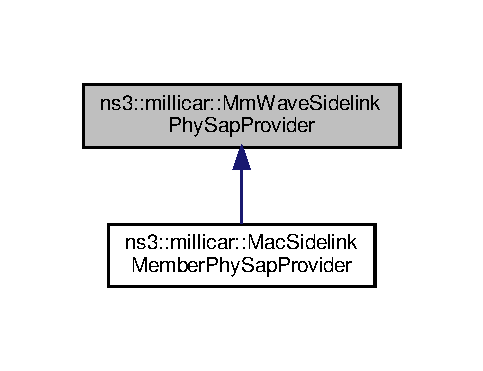
\includegraphics[width=232pt]{classns3_1_1millicar_1_1MmWaveSidelinkPhySapProvider__inherit__graph}
\end{center}
\end{figure}
\subsection*{Public Member Functions}
\begin{DoxyCompactItemize}
\item 
virtual void \hyperlink{classns3_1_1millicar_1_1MmWaveSidelinkPhySapProvider_acba80cb123b9eb0fcacefde35a91909d}{Add\+Transport\+Block} (Ptr$<$ Packet\+Burst $>$ pb, mmwave\+::\+Tti\+Alloc\+Info info)=0
\begin{DoxyCompactList}\small\item\em Called by the upper layers to fill P\+HY\textquotesingle{}s buffer. \end{DoxyCompactList}\item 
virtual void \hyperlink{classns3_1_1millicar_1_1MmWaveSidelinkPhySapProvider_a1c791fea7b4457a39428f3da49eaf6b8}{Prepare\+For\+Reception} (uint16\+\_\+t rnti)=0
\begin{DoxyCompactList}\small\item\em Called by the upper layer to prepare the P\+HY for the reception from another device. \end{DoxyCompactList}\end{DoxyCompactItemize}


\subsection{Member Function Documentation}
\mbox{\Hypertarget{classns3_1_1millicar_1_1MmWaveSidelinkPhySapProvider_acba80cb123b9eb0fcacefde35a91909d}\label{classns3_1_1millicar_1_1MmWaveSidelinkPhySapProvider_acba80cb123b9eb0fcacefde35a91909d}} 
\index{ns3\+::millicar\+::\+Mm\+Wave\+Sidelink\+Phy\+Sap\+Provider@{ns3\+::millicar\+::\+Mm\+Wave\+Sidelink\+Phy\+Sap\+Provider}!Add\+Transport\+Block@{Add\+Transport\+Block}}
\index{Add\+Transport\+Block@{Add\+Transport\+Block}!ns3\+::millicar\+::\+Mm\+Wave\+Sidelink\+Phy\+Sap\+Provider@{ns3\+::millicar\+::\+Mm\+Wave\+Sidelink\+Phy\+Sap\+Provider}}
\subsubsection{\texorpdfstring{Add\+Transport\+Block()}{AddTransportBlock()}}
{\footnotesize\ttfamily virtual void ns3\+::millicar\+::\+Mm\+Wave\+Sidelink\+Phy\+Sap\+Provider\+::\+Add\+Transport\+Block (\begin{DoxyParamCaption}\item[{Ptr$<$ Packet\+Burst $>$}]{pb,  }\item[{mmwave\+::\+Tti\+Alloc\+Info}]{info }\end{DoxyParamCaption})\hspace{0.3cm}{\ttfamily [pure virtual]}}



Called by the upper layers to fill P\+HY\textquotesingle{}s buffer. 


\begin{DoxyParams}{Parameters}
{\em pb} & burst of packets to be forwarded to the P\+HY layer \\
\hline
{\em info} & information about slot allocation necessary to determine the transmission parameters \\
\hline
\end{DoxyParams}


Implemented in \hyperlink{classns3_1_1millicar_1_1MacSidelinkMemberPhySapProvider_ad6a8a2b3021363432e870d4051448b15}{ns3\+::millicar\+::\+Mac\+Sidelink\+Member\+Phy\+Sap\+Provider}.

\mbox{\Hypertarget{classns3_1_1millicar_1_1MmWaveSidelinkPhySapProvider_a1c791fea7b4457a39428f3da49eaf6b8}\label{classns3_1_1millicar_1_1MmWaveSidelinkPhySapProvider_a1c791fea7b4457a39428f3da49eaf6b8}} 
\index{ns3\+::millicar\+::\+Mm\+Wave\+Sidelink\+Phy\+Sap\+Provider@{ns3\+::millicar\+::\+Mm\+Wave\+Sidelink\+Phy\+Sap\+Provider}!Prepare\+For\+Reception@{Prepare\+For\+Reception}}
\index{Prepare\+For\+Reception@{Prepare\+For\+Reception}!ns3\+::millicar\+::\+Mm\+Wave\+Sidelink\+Phy\+Sap\+Provider@{ns3\+::millicar\+::\+Mm\+Wave\+Sidelink\+Phy\+Sap\+Provider}}
\subsubsection{\texorpdfstring{Prepare\+For\+Reception()}{PrepareForReception()}}
{\footnotesize\ttfamily virtual void ns3\+::millicar\+::\+Mm\+Wave\+Sidelink\+Phy\+Sap\+Provider\+::\+Prepare\+For\+Reception (\begin{DoxyParamCaption}\item[{uint16\+\_\+t}]{rnti }\end{DoxyParamCaption})\hspace{0.3cm}{\ttfamily [pure virtual]}}



Called by the upper layer to prepare the P\+HY for the reception from another device. 


\begin{DoxyParams}{Parameters}
{\em rnti} & the rnti of the transmitting device \\
\hline
\end{DoxyParams}


Implemented in \hyperlink{classns3_1_1millicar_1_1MacSidelinkMemberPhySapProvider_afe0a87706052aabc88e7c4fbd4cc7a02}{ns3\+::millicar\+::\+Mac\+Sidelink\+Member\+Phy\+Sap\+Provider}.



The documentation for this class was generated from the following file\+:\begin{DoxyCompactItemize}
\item 
model/mmwave-\/sidelink-\/sap.\+h\end{DoxyCompactItemize}

\hypertarget{classns3_1_1millicar_1_1MmWaveSidelinkPhySapUser}{}\section{ns3\+:\+:millicar\+:\+:Mm\+Wave\+Sidelink\+Phy\+Sap\+User Class Reference}
\label{classns3_1_1millicar_1_1MmWaveSidelinkPhySapUser}\index{ns3\+::millicar\+::\+Mm\+Wave\+Sidelink\+Phy\+Sap\+User@{ns3\+::millicar\+::\+Mm\+Wave\+Sidelink\+Phy\+Sap\+User}}


Inheritance diagram for ns3\+:\+:millicar\+:\+:Mm\+Wave\+Sidelink\+Phy\+Sap\+User\+:\nopagebreak
\begin{figure}[H]
\begin{center}
\leavevmode
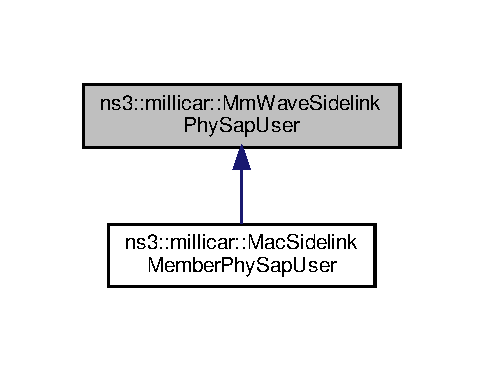
\includegraphics[width=232pt]{classns3_1_1millicar_1_1MmWaveSidelinkPhySapUser__inherit__graph}
\end{center}
\end{figure}
\subsection*{Public Member Functions}
\begin{DoxyCompactItemize}
\item 
virtual void \hyperlink{classns3_1_1millicar_1_1MmWaveSidelinkPhySapUser_ac0e4d40ace55e47cb3fb54d09c80fe06}{Receive\+Phy\+Pdu} (Ptr$<$ Packet $>$ p)=0
\begin{DoxyCompactList}\small\item\em Called by the P\+HY to notify the M\+AC of the reception of a new P\+H\+Y-\/\+P\+DU. \end{DoxyCompactList}\item 
virtual void \hyperlink{classns3_1_1millicar_1_1MmWaveSidelinkPhySapUser_a237ec6c8c7496a3e021d22393ba7fc61}{Slot\+Indication} (mmwave\+::\+Sfn\+Sf timing\+Info)=0
\begin{DoxyCompactList}\small\item\em Trigger the start from a new slot (input from P\+HY layer) \end{DoxyCompactList}\item 
virtual void \hyperlink{classns3_1_1millicar_1_1MmWaveSidelinkPhySapUser_aedb96411ce5a46589df517b1aa272d97}{Sl\+Sinr\+Report} (const Spectrum\+Value \&sinr, uint16\+\_\+t rnti, uint8\+\_\+t num\+Sym, uint32\+\_\+t tb\+Size)=0
\begin{DoxyCompactList}\small\item\em Reports the S\+I\+NR meausured with a certain device. \end{DoxyCompactList}\end{DoxyCompactItemize}


\subsection{Member Function Documentation}
\mbox{\Hypertarget{classns3_1_1millicar_1_1MmWaveSidelinkPhySapUser_ac0e4d40ace55e47cb3fb54d09c80fe06}\label{classns3_1_1millicar_1_1MmWaveSidelinkPhySapUser_ac0e4d40ace55e47cb3fb54d09c80fe06}} 
\index{ns3\+::millicar\+::\+Mm\+Wave\+Sidelink\+Phy\+Sap\+User@{ns3\+::millicar\+::\+Mm\+Wave\+Sidelink\+Phy\+Sap\+User}!Receive\+Phy\+Pdu@{Receive\+Phy\+Pdu}}
\index{Receive\+Phy\+Pdu@{Receive\+Phy\+Pdu}!ns3\+::millicar\+::\+Mm\+Wave\+Sidelink\+Phy\+Sap\+User@{ns3\+::millicar\+::\+Mm\+Wave\+Sidelink\+Phy\+Sap\+User}}
\subsubsection{\texorpdfstring{Receive\+Phy\+Pdu()}{ReceivePhyPdu()}}
{\footnotesize\ttfamily virtual void ns3\+::millicar\+::\+Mm\+Wave\+Sidelink\+Phy\+Sap\+User\+::\+Receive\+Phy\+Pdu (\begin{DoxyParamCaption}\item[{Ptr$<$ Packet $>$}]{p }\end{DoxyParamCaption})\hspace{0.3cm}{\ttfamily [pure virtual]}}



Called by the P\+HY to notify the M\+AC of the reception of a new P\+H\+Y-\/\+P\+DU. 


\begin{DoxyParams}{Parameters}
{\em p} & packet \\
\hline
\end{DoxyParams}


Implemented in \hyperlink{classns3_1_1millicar_1_1MacSidelinkMemberPhySapUser_a430a252dfedeea5228eab8e62af82960}{ns3\+::millicar\+::\+Mac\+Sidelink\+Member\+Phy\+Sap\+User}.

\mbox{\Hypertarget{classns3_1_1millicar_1_1MmWaveSidelinkPhySapUser_a237ec6c8c7496a3e021d22393ba7fc61}\label{classns3_1_1millicar_1_1MmWaveSidelinkPhySapUser_a237ec6c8c7496a3e021d22393ba7fc61}} 
\index{ns3\+::millicar\+::\+Mm\+Wave\+Sidelink\+Phy\+Sap\+User@{ns3\+::millicar\+::\+Mm\+Wave\+Sidelink\+Phy\+Sap\+User}!Slot\+Indication@{Slot\+Indication}}
\index{Slot\+Indication@{Slot\+Indication}!ns3\+::millicar\+::\+Mm\+Wave\+Sidelink\+Phy\+Sap\+User@{ns3\+::millicar\+::\+Mm\+Wave\+Sidelink\+Phy\+Sap\+User}}
\subsubsection{\texorpdfstring{Slot\+Indication()}{SlotIndication()}}
{\footnotesize\ttfamily virtual void ns3\+::millicar\+::\+Mm\+Wave\+Sidelink\+Phy\+Sap\+User\+::\+Slot\+Indication (\begin{DoxyParamCaption}\item[{mmwave\+::\+Sfn\+Sf}]{timing\+Info }\end{DoxyParamCaption})\hspace{0.3cm}{\ttfamily [pure virtual]}}



Trigger the start from a new slot (input from P\+HY layer) 


\begin{DoxyParams}{Parameters}
{\em timing\+Info} & the structure containing the timing information \\
\hline
\end{DoxyParams}


Implemented in \hyperlink{classns3_1_1millicar_1_1MacSidelinkMemberPhySapUser_ae204b07ff1b6fcd8d50dc71d21b51278}{ns3\+::millicar\+::\+Mac\+Sidelink\+Member\+Phy\+Sap\+User}.

\mbox{\Hypertarget{classns3_1_1millicar_1_1MmWaveSidelinkPhySapUser_aedb96411ce5a46589df517b1aa272d97}\label{classns3_1_1millicar_1_1MmWaveSidelinkPhySapUser_aedb96411ce5a46589df517b1aa272d97}} 
\index{ns3\+::millicar\+::\+Mm\+Wave\+Sidelink\+Phy\+Sap\+User@{ns3\+::millicar\+::\+Mm\+Wave\+Sidelink\+Phy\+Sap\+User}!Sl\+Sinr\+Report@{Sl\+Sinr\+Report}}
\index{Sl\+Sinr\+Report@{Sl\+Sinr\+Report}!ns3\+::millicar\+::\+Mm\+Wave\+Sidelink\+Phy\+Sap\+User@{ns3\+::millicar\+::\+Mm\+Wave\+Sidelink\+Phy\+Sap\+User}}
\subsubsection{\texorpdfstring{Sl\+Sinr\+Report()}{SlSinrReport()}}
{\footnotesize\ttfamily virtual void ns3\+::millicar\+::\+Mm\+Wave\+Sidelink\+Phy\+Sap\+User\+::\+Sl\+Sinr\+Report (\begin{DoxyParamCaption}\item[{const Spectrum\+Value \&}]{sinr,  }\item[{uint16\+\_\+t}]{rnti,  }\item[{uint8\+\_\+t}]{num\+Sym,  }\item[{uint32\+\_\+t}]{tb\+Size }\end{DoxyParamCaption})\hspace{0.3cm}{\ttfamily [pure virtual]}}



Reports the S\+I\+NR meausured with a certain device. 


\begin{DoxyParams}{Parameters}
{\em sinr} & the S\+I\+NR \\
\hline
{\em rnti} & R\+N\+TI of the transmitting device \\
\hline
{\em num\+Sym} & size of the transport block that generated the report in number of O\+F\+DM symbols \\
\hline
{\em tb\+Size} & size of the transport block that generated the report in number of bytes \\
\hline
\end{DoxyParams}


Implemented in \hyperlink{classns3_1_1millicar_1_1MacSidelinkMemberPhySapUser_a68dd0cadd60b7bf0d2a3ac34a15a8e4c}{ns3\+::millicar\+::\+Mac\+Sidelink\+Member\+Phy\+Sap\+User}.



The documentation for this class was generated from the following file\+:\begin{DoxyCompactItemize}
\item 
model/mmwave-\/sidelink-\/sap.\+h\end{DoxyCompactItemize}

\hypertarget{classns3_1_1millicar_1_1MmWaveSidelinkSpectrumPhy}{}\section{ns3\+:\+:millicar\+:\+:Mm\+Wave\+Sidelink\+Spectrum\+Phy Class Reference}
\label{classns3_1_1millicar_1_1MmWaveSidelinkSpectrumPhy}\index{ns3\+::millicar\+::\+Mm\+Wave\+Sidelink\+Spectrum\+Phy@{ns3\+::millicar\+::\+Mm\+Wave\+Sidelink\+Spectrum\+Phy}}


{\ttfamily \#include $<$mmwave-\/sidelink-\/spectrum-\/phy.\+h$>$}



Inheritance diagram for ns3\+:\+:millicar\+:\+:Mm\+Wave\+Sidelink\+Spectrum\+Phy\+:\nopagebreak
\begin{figure}[H]
\begin{center}
\leavevmode
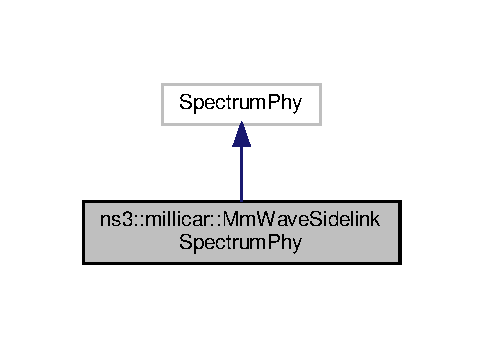
\includegraphics[width=232pt]{classns3_1_1millicar_1_1MmWaveSidelinkSpectrumPhy__inherit__graph}
\end{center}
\end{figure}


Collaboration diagram for ns3\+:\+:millicar\+:\+:Mm\+Wave\+Sidelink\+Spectrum\+Phy\+:\nopagebreak
\begin{figure}[H]
\begin{center}
\leavevmode
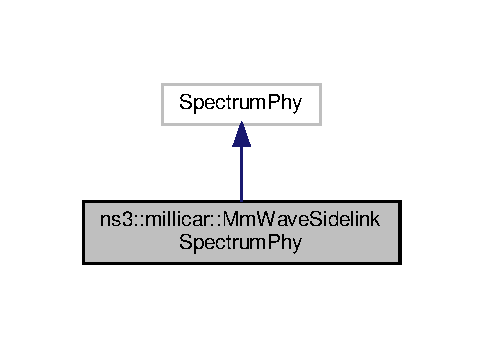
\includegraphics[width=232pt]{classns3_1_1millicar_1_1MmWaveSidelinkSpectrumPhy__coll__graph}
\end{center}
\end{figure}
\subsection*{Public Types}
\begin{DoxyCompactItemize}
\item 
enum \hyperlink{classns3_1_1millicar_1_1MmWaveSidelinkSpectrumPhy_a242b6a18fa64a2063ee36fd2d7b44e84}{State} \{ {\bfseries I\+D\+LE} = 0, 
{\bfseries TX}, 
{\bfseries R\+X\+\_\+\+D\+A\+TA}, 
{\bfseries R\+X\+\_\+\+C\+T\+RL}
 \}
\end{DoxyCompactItemize}
\subsection*{Public Member Functions}
\begin{DoxyCompactItemize}
\item 
\mbox{\Hypertarget{classns3_1_1millicar_1_1MmWaveSidelinkSpectrumPhy_a868e28c54b93d5f2e321fd5c8e070991}\label{classns3_1_1millicar_1_1MmWaveSidelinkSpectrumPhy_a868e28c54b93d5f2e321fd5c8e070991}} 
virtual void {\bfseries Do\+Dispose} ()
\item 
\mbox{\Hypertarget{classns3_1_1millicar_1_1MmWaveSidelinkSpectrumPhy_a912fab89ea4a35b2e72ee84f72f97c83}\label{classns3_1_1millicar_1_1MmWaveSidelinkSpectrumPhy_a912fab89ea4a35b2e72ee84f72f97c83}} 
void {\bfseries Reset} ()
\item 
\mbox{\Hypertarget{classns3_1_1millicar_1_1MmWaveSidelinkSpectrumPhy_a824c1d2a9515d14decefc949f30156d7}\label{classns3_1_1millicar_1_1MmWaveSidelinkSpectrumPhy_a824c1d2a9515d14decefc949f30156d7}} 
void {\bfseries Reset\+Spectrum\+Model} ()
\item 
void \hyperlink{classns3_1_1millicar_1_1MmWaveSidelinkSpectrumPhy_a965a2aa951f0127652f916d46760ab59}{Set\+Device} (Ptr$<$ Net\+Device $>$ d)
\item 
Ptr$<$ Net\+Device $>$ \hyperlink{classns3_1_1millicar_1_1MmWaveSidelinkSpectrumPhy_ace3f5a3bf2de94bb325ad37c1738dfa3}{Get\+Device} () const
\item 
void \hyperlink{classns3_1_1millicar_1_1MmWaveSidelinkSpectrumPhy_a9892bb8ce4fccbc6e3ea04b90f453715}{Set\+Mobility} (Ptr$<$ Mobility\+Model $>$ m)
\item 
Ptr$<$ Mobility\+Model $>$ \hyperlink{classns3_1_1millicar_1_1MmWaveSidelinkSpectrumPhy_a32642929c3eafdf82ae27e6b9ece29cf}{Get\+Mobility} ()
\item 
void \hyperlink{classns3_1_1millicar_1_1MmWaveSidelinkSpectrumPhy_a52aa6d4f22a306aeb405f126bb5c6277}{Set\+Channel} (Ptr$<$ Spectrum\+Channel $>$ c)
\item 
Ptr$<$ const Spectrum\+Model $>$ \hyperlink{classns3_1_1millicar_1_1MmWaveSidelinkSpectrumPhy_adf0968d0659b5790d71a1b41df56c221}{Get\+Rx\+Spectrum\+Model} () const
\item 
Ptr$<$ Antenna\+Model $>$ \hyperlink{classns3_1_1millicar_1_1MmWaveSidelinkSpectrumPhy_a1a7c251de6b22c5afbafcf5937a12082}{Get\+Rx\+Antenna} ()
\item 
void \hyperlink{classns3_1_1millicar_1_1MmWaveSidelinkSpectrumPhy_a3d60ad512ba0df1c26814dad5a241fff}{Set\+Antenna} (Ptr$<$ Antenna\+Model $>$ a)
\item 
\mbox{\Hypertarget{classns3_1_1millicar_1_1MmWaveSidelinkSpectrumPhy_aab37ea813e418ef5eb11fffee564612a}\label{classns3_1_1millicar_1_1MmWaveSidelinkSpectrumPhy_aab37ea813e418ef5eb11fffee564612a}} 
void {\bfseries Set\+Noise\+Power\+Spectral\+Density} (Ptr$<$ const Spectrum\+Value $>$ noise\+Psd)
\item 
\mbox{\Hypertarget{classns3_1_1millicar_1_1MmWaveSidelinkSpectrumPhy_aca5b41a007ac964361cf0fec5b194739}\label{classns3_1_1millicar_1_1MmWaveSidelinkSpectrumPhy_aca5b41a007ac964361cf0fec5b194739}} 
void {\bfseries Set\+Tx\+Power\+Spectral\+Density} (Ptr$<$ Spectrum\+Value $>$ Tx\+Psd)
\item 
\mbox{\Hypertarget{classns3_1_1millicar_1_1MmWaveSidelinkSpectrumPhy_ad37a4e747310a48d149d95f73ed390b1}\label{classns3_1_1millicar_1_1MmWaveSidelinkSpectrumPhy_ad37a4e747310a48d149d95f73ed390b1}} 
void {\bfseries Start\+Rx} (Ptr$<$ Spectrum\+Signal\+Parameters $>$ params)
\item 
void \hyperlink{classns3_1_1millicar_1_1MmWaveSidelinkSpectrumPhy_a22f0761f08f5f08dda1de1c778832f5a}{Start\+Rx\+Data} (Ptr$<$ \hyperlink{structns3_1_1millicar_1_1MmWaveSidelinkSpectrumSignalParameters}{Mm\+Wave\+Sidelink\+Spectrum\+Signal\+Parameters} $>$ params)
\begin{DoxyCompactList}\small\item\em Start receive data function. \end{DoxyCompactList}\item 
Ptr$<$ Spectrum\+Channel $>$ \hyperlink{classns3_1_1millicar_1_1MmWaveSidelinkSpectrumPhy_a831e25da1a41abd432e7e412abdb2e90}{Get\+Spectrum\+Channel} ()
\begin{DoxyCompactList}\small\item\em Start receive control function. \end{DoxyCompactList}\item 
bool \hyperlink{classns3_1_1millicar_1_1MmWaveSidelinkSpectrumPhy_ae3703a686eae8ac683c726aeb93cfb6b}{Start\+Tx\+Data\+Frames} (Ptr$<$ Packet\+Burst $>$ pb, Time duration, uint8\+\_\+t mcs, uint32\+\_\+t size, uint8\+\_\+t num\+Sym, uint16\+\_\+t sender\+Rnti, uint16\+\_\+t destination\+Rnti, std\+::vector$<$ int $>$ rb\+Bitmap)
\item 
void \hyperlink{classns3_1_1millicar_1_1MmWaveSidelinkSpectrumPhy_a1d67dd214d625371084795980d021a8c}{Set\+Phy\+Rx\+Data\+End\+Ok\+Callback} (Mm\+Wave\+Phy\+Rx\+Data\+End\+Ok\+Callback c)
\item 
void \hyperlink{classns3_1_1millicar_1_1MmWaveSidelinkSpectrumPhy_ae88ae2ce12c9384f8dfd2dddfa6f8049}{Set\+Sidelink\+Sinr\+Report\+Callback} (Mm\+Wave\+Sidelink\+Sinr\+Report\+Callback c)
\item 
void \hyperlink{classns3_1_1millicar_1_1MmWaveSidelinkSpectrumPhy_a2a88ce71bf01205dfcb564f9de6c8830}{Add\+Data\+Power\+Chunk\+Processor} (Ptr$<$ mmwave\+::mm\+Wave\+Chunk\+Processor $>$ p)
\item 
void \hyperlink{classns3_1_1millicar_1_1MmWaveSidelinkSpectrumPhy_acf9d93deaf45b27e497494c9b723584a}{Add\+Data\+Sinr\+Chunk\+Processor} (Ptr$<$ mmwave\+::mm\+Wave\+Chunk\+Processor $>$ p)
\item 
void \hyperlink{classns3_1_1millicar_1_1MmWaveSidelinkSpectrumPhy_a504ec60aaf6a7115b78013e1e3d18c8c}{Update\+Sinr\+Perceived} (const Spectrum\+Value \&sinr)
\item 
void \hyperlink{classns3_1_1millicar_1_1MmWaveSidelinkSpectrumPhy_aa646318e906fee1914c297eb169dd2cc}{Configure\+Beamforming} (Ptr$<$ Net\+Device $>$ dev)
\end{DoxyCompactItemize}
\subsection*{Static Public Member Functions}
\begin{DoxyCompactItemize}
\item 
static Type\+Id \hyperlink{classns3_1_1millicar_1_1MmWaveSidelinkSpectrumPhy_a751fd1b25b484a1a8d32d62d2545069c}{Get\+Type\+Id} (void)
\begin{DoxyCompactList}\small\item\em Get the type ID. \end{DoxyCompactList}\end{DoxyCompactItemize}


\subsection{Detailed Description}
The \hyperlink{classns3_1_1millicar_1_1MmWaveSidelinkSpectrumPhy}{Mm\+Wave\+Sidelink\+Spectrum\+Phy} models the physical layer of sidelink mode of vehicular networks exploiting mmwave band. 

\subsection{Member Enumeration Documentation}
\mbox{\Hypertarget{classns3_1_1millicar_1_1MmWaveSidelinkSpectrumPhy_a242b6a18fa64a2063ee36fd2d7b44e84}\label{classns3_1_1millicar_1_1MmWaveSidelinkSpectrumPhy_a242b6a18fa64a2063ee36fd2d7b44e84}} 
\index{ns3\+::millicar\+::\+Mm\+Wave\+Sidelink\+Spectrum\+Phy@{ns3\+::millicar\+::\+Mm\+Wave\+Sidelink\+Spectrum\+Phy}!State@{State}}
\index{State@{State}!ns3\+::millicar\+::\+Mm\+Wave\+Sidelink\+Spectrum\+Phy@{ns3\+::millicar\+::\+Mm\+Wave\+Sidelink\+Spectrum\+Phy}}
\subsubsection{\texorpdfstring{State}{State}}
{\footnotesize\ttfamily enum \hyperlink{classns3_1_1millicar_1_1MmWaveSidelinkSpectrumPhy_a242b6a18fa64a2063ee36fd2d7b44e84}{ns3\+::millicar\+::\+Mm\+Wave\+Sidelink\+Spectrum\+Phy\+::\+State}}

P\+HY states 

\subsection{Member Function Documentation}
\mbox{\Hypertarget{classns3_1_1millicar_1_1MmWaveSidelinkSpectrumPhy_a2a88ce71bf01205dfcb564f9de6c8830}\label{classns3_1_1millicar_1_1MmWaveSidelinkSpectrumPhy_a2a88ce71bf01205dfcb564f9de6c8830}} 
\index{ns3\+::millicar\+::\+Mm\+Wave\+Sidelink\+Spectrum\+Phy@{ns3\+::millicar\+::\+Mm\+Wave\+Sidelink\+Spectrum\+Phy}!Add\+Data\+Power\+Chunk\+Processor@{Add\+Data\+Power\+Chunk\+Processor}}
\index{Add\+Data\+Power\+Chunk\+Processor@{Add\+Data\+Power\+Chunk\+Processor}!ns3\+::millicar\+::\+Mm\+Wave\+Sidelink\+Spectrum\+Phy@{ns3\+::millicar\+::\+Mm\+Wave\+Sidelink\+Spectrum\+Phy}}
\subsubsection{\texorpdfstring{Add\+Data\+Power\+Chunk\+Processor()}{AddDataPowerChunkProcessor()}}
{\footnotesize\ttfamily void ns3\+::millicar\+::\+Mm\+Wave\+Sidelink\+Spectrum\+Phy\+::\+Add\+Data\+Power\+Chunk\+Processor (\begin{DoxyParamCaption}\item[{Ptr$<$ mmwave\+::mm\+Wave\+Chunk\+Processor $>$}]{p }\end{DoxyParamCaption})}


\begin{DoxyParams}{Parameters}
{\em p} & the new Chunk\+Processor to be added to the Data Channel power processing chain \\
\hline
\end{DoxyParams}
\mbox{\Hypertarget{classns3_1_1millicar_1_1MmWaveSidelinkSpectrumPhy_acf9d93deaf45b27e497494c9b723584a}\label{classns3_1_1millicar_1_1MmWaveSidelinkSpectrumPhy_acf9d93deaf45b27e497494c9b723584a}} 
\index{ns3\+::millicar\+::\+Mm\+Wave\+Sidelink\+Spectrum\+Phy@{ns3\+::millicar\+::\+Mm\+Wave\+Sidelink\+Spectrum\+Phy}!Add\+Data\+Sinr\+Chunk\+Processor@{Add\+Data\+Sinr\+Chunk\+Processor}}
\index{Add\+Data\+Sinr\+Chunk\+Processor@{Add\+Data\+Sinr\+Chunk\+Processor}!ns3\+::millicar\+::\+Mm\+Wave\+Sidelink\+Spectrum\+Phy@{ns3\+::millicar\+::\+Mm\+Wave\+Sidelink\+Spectrum\+Phy}}
\subsubsection{\texorpdfstring{Add\+Data\+Sinr\+Chunk\+Processor()}{AddDataSinrChunkProcessor()}}
{\footnotesize\ttfamily void ns3\+::millicar\+::\+Mm\+Wave\+Sidelink\+Spectrum\+Phy\+::\+Add\+Data\+Sinr\+Chunk\+Processor (\begin{DoxyParamCaption}\item[{Ptr$<$ mmwave\+::mm\+Wave\+Chunk\+Processor $>$}]{p }\end{DoxyParamCaption})}


\begin{DoxyParams}{Parameters}
{\em p} & the new Chunk\+Processor to be added to the data processing chain \\
\hline
\end{DoxyParams}
\mbox{\Hypertarget{classns3_1_1millicar_1_1MmWaveSidelinkSpectrumPhy_aa646318e906fee1914c297eb169dd2cc}\label{classns3_1_1millicar_1_1MmWaveSidelinkSpectrumPhy_aa646318e906fee1914c297eb169dd2cc}} 
\index{ns3\+::millicar\+::\+Mm\+Wave\+Sidelink\+Spectrum\+Phy@{ns3\+::millicar\+::\+Mm\+Wave\+Sidelink\+Spectrum\+Phy}!Configure\+Beamforming@{Configure\+Beamforming}}
\index{Configure\+Beamforming@{Configure\+Beamforming}!ns3\+::millicar\+::\+Mm\+Wave\+Sidelink\+Spectrum\+Phy@{ns3\+::millicar\+::\+Mm\+Wave\+Sidelink\+Spectrum\+Phy}}
\subsubsection{\texorpdfstring{Configure\+Beamforming()}{ConfigureBeamforming()}}
{\footnotesize\ttfamily void ns3\+::millicar\+::\+Mm\+Wave\+Sidelink\+Spectrum\+Phy\+::\+Configure\+Beamforming (\begin{DoxyParamCaption}\item[{Ptr$<$ Net\+Device $>$}]{dev }\end{DoxyParamCaption})}

Configure the beamforming to communicate with a specific device 
\begin{DoxyParams}{Parameters}
{\em dev} & the device we want to communicate with \\
\hline
\end{DoxyParams}
\mbox{\Hypertarget{classns3_1_1millicar_1_1MmWaveSidelinkSpectrumPhy_ace3f5a3bf2de94bb325ad37c1738dfa3}\label{classns3_1_1millicar_1_1MmWaveSidelinkSpectrumPhy_ace3f5a3bf2de94bb325ad37c1738dfa3}} 
\index{ns3\+::millicar\+::\+Mm\+Wave\+Sidelink\+Spectrum\+Phy@{ns3\+::millicar\+::\+Mm\+Wave\+Sidelink\+Spectrum\+Phy}!Get\+Device@{Get\+Device}}
\index{Get\+Device@{Get\+Device}!ns3\+::millicar\+::\+Mm\+Wave\+Sidelink\+Spectrum\+Phy@{ns3\+::millicar\+::\+Mm\+Wave\+Sidelink\+Spectrum\+Phy}}
\subsubsection{\texorpdfstring{Get\+Device()}{GetDevice()}}
{\footnotesize\ttfamily Ptr$<$ Net\+Device $>$ ns3\+::millicar\+::\+Mm\+Wave\+Sidelink\+Spectrum\+Phy\+::\+Get\+Device (\begin{DoxyParamCaption}{ }\end{DoxyParamCaption}) const}

Get the associated Net\+Device instance

\begin{DoxyReturn}{Returns}
a Ptr to the associated Net\+Device instance 
\end{DoxyReturn}
\mbox{\Hypertarget{classns3_1_1millicar_1_1MmWaveSidelinkSpectrumPhy_a32642929c3eafdf82ae27e6b9ece29cf}\label{classns3_1_1millicar_1_1MmWaveSidelinkSpectrumPhy_a32642929c3eafdf82ae27e6b9ece29cf}} 
\index{ns3\+::millicar\+::\+Mm\+Wave\+Sidelink\+Spectrum\+Phy@{ns3\+::millicar\+::\+Mm\+Wave\+Sidelink\+Spectrum\+Phy}!Get\+Mobility@{Get\+Mobility}}
\index{Get\+Mobility@{Get\+Mobility}!ns3\+::millicar\+::\+Mm\+Wave\+Sidelink\+Spectrum\+Phy@{ns3\+::millicar\+::\+Mm\+Wave\+Sidelink\+Spectrum\+Phy}}
\subsubsection{\texorpdfstring{Get\+Mobility()}{GetMobility()}}
{\footnotesize\ttfamily Ptr$<$ Mobility\+Model $>$ ns3\+::millicar\+::\+Mm\+Wave\+Sidelink\+Spectrum\+Phy\+::\+Get\+Mobility (\begin{DoxyParamCaption}{ }\end{DoxyParamCaption})}

Get the associated Mobility\+Model instance

\begin{DoxyReturn}{Returns}
a Ptr to the associated Mobility\+Model instance 
\end{DoxyReturn}
\mbox{\Hypertarget{classns3_1_1millicar_1_1MmWaveSidelinkSpectrumPhy_a1a7c251de6b22c5afbafcf5937a12082}\label{classns3_1_1millicar_1_1MmWaveSidelinkSpectrumPhy_a1a7c251de6b22c5afbafcf5937a12082}} 
\index{ns3\+::millicar\+::\+Mm\+Wave\+Sidelink\+Spectrum\+Phy@{ns3\+::millicar\+::\+Mm\+Wave\+Sidelink\+Spectrum\+Phy}!Get\+Rx\+Antenna@{Get\+Rx\+Antenna}}
\index{Get\+Rx\+Antenna@{Get\+Rx\+Antenna}!ns3\+::millicar\+::\+Mm\+Wave\+Sidelink\+Spectrum\+Phy@{ns3\+::millicar\+::\+Mm\+Wave\+Sidelink\+Spectrum\+Phy}}
\subsubsection{\texorpdfstring{Get\+Rx\+Antenna()}{GetRxAntenna()}}
{\footnotesize\ttfamily Ptr$<$ Antenna\+Model $>$ ns3\+::millicar\+::\+Mm\+Wave\+Sidelink\+Spectrum\+Phy\+::\+Get\+Rx\+Antenna (\begin{DoxyParamCaption}{ }\end{DoxyParamCaption})}

Get the Antenna\+Model used by the Net\+Device for reception

\begin{DoxyReturn}{Returns}
a Ptr to the Antenna\+Model used by the Net\+Device for reception 
\end{DoxyReturn}
\mbox{\Hypertarget{classns3_1_1millicar_1_1MmWaveSidelinkSpectrumPhy_adf0968d0659b5790d71a1b41df56c221}\label{classns3_1_1millicar_1_1MmWaveSidelinkSpectrumPhy_adf0968d0659b5790d71a1b41df56c221}} 
\index{ns3\+::millicar\+::\+Mm\+Wave\+Sidelink\+Spectrum\+Phy@{ns3\+::millicar\+::\+Mm\+Wave\+Sidelink\+Spectrum\+Phy}!Get\+Rx\+Spectrum\+Model@{Get\+Rx\+Spectrum\+Model}}
\index{Get\+Rx\+Spectrum\+Model@{Get\+Rx\+Spectrum\+Model}!ns3\+::millicar\+::\+Mm\+Wave\+Sidelink\+Spectrum\+Phy@{ns3\+::millicar\+::\+Mm\+Wave\+Sidelink\+Spectrum\+Phy}}
\subsubsection{\texorpdfstring{Get\+Rx\+Spectrum\+Model()}{GetRxSpectrumModel()}}
{\footnotesize\ttfamily Ptr$<$ const Spectrum\+Model $>$ ns3\+::millicar\+::\+Mm\+Wave\+Sidelink\+Spectrum\+Phy\+::\+Get\+Rx\+Spectrum\+Model (\begin{DoxyParamCaption}{ }\end{DoxyParamCaption}) const}

\begin{DoxyReturn}{Returns}
returns the Spectrum\+Model that this Spectrum\+Phy expects to be used for all Spectrum\+Values that are passed to Start\+Rx. If 0 is returned, it means that any model will be accepted. 
\end{DoxyReturn}
\mbox{\Hypertarget{classns3_1_1millicar_1_1MmWaveSidelinkSpectrumPhy_a831e25da1a41abd432e7e412abdb2e90}\label{classns3_1_1millicar_1_1MmWaveSidelinkSpectrumPhy_a831e25da1a41abd432e7e412abdb2e90}} 
\index{ns3\+::millicar\+::\+Mm\+Wave\+Sidelink\+Spectrum\+Phy@{ns3\+::millicar\+::\+Mm\+Wave\+Sidelink\+Spectrum\+Phy}!Get\+Spectrum\+Channel@{Get\+Spectrum\+Channel}}
\index{Get\+Spectrum\+Channel@{Get\+Spectrum\+Channel}!ns3\+::millicar\+::\+Mm\+Wave\+Sidelink\+Spectrum\+Phy@{ns3\+::millicar\+::\+Mm\+Wave\+Sidelink\+Spectrum\+Phy}}
\subsubsection{\texorpdfstring{Get\+Spectrum\+Channel()}{GetSpectrumChannel()}}
{\footnotesize\ttfamily Ptr$<$ Spectrum\+Channel $>$ ns3\+::millicar\+::\+Mm\+Wave\+Sidelink\+Spectrum\+Phy\+::\+Get\+Spectrum\+Channel (\begin{DoxyParamCaption}{ }\end{DoxyParamCaption})}



Start receive control function. 


\begin{DoxyParams}{Parameters}
{\em params} & Ptr$<$\+Spectrum\+Signal\+Parameters$>$ \\
\hline
\end{DoxyParams}
\mbox{\Hypertarget{classns3_1_1millicar_1_1MmWaveSidelinkSpectrumPhy_a751fd1b25b484a1a8d32d62d2545069c}\label{classns3_1_1millicar_1_1MmWaveSidelinkSpectrumPhy_a751fd1b25b484a1a8d32d62d2545069c}} 
\index{ns3\+::millicar\+::\+Mm\+Wave\+Sidelink\+Spectrum\+Phy@{ns3\+::millicar\+::\+Mm\+Wave\+Sidelink\+Spectrum\+Phy}!Get\+Type\+Id@{Get\+Type\+Id}}
\index{Get\+Type\+Id@{Get\+Type\+Id}!ns3\+::millicar\+::\+Mm\+Wave\+Sidelink\+Spectrum\+Phy@{ns3\+::millicar\+::\+Mm\+Wave\+Sidelink\+Spectrum\+Phy}}
\subsubsection{\texorpdfstring{Get\+Type\+Id()}{GetTypeId()}}
{\footnotesize\ttfamily Type\+Id ns3\+::millicar\+::\+Mm\+Wave\+Sidelink\+Spectrum\+Phy\+::\+Get\+Type\+Id (\begin{DoxyParamCaption}\item[{void}]{ }\end{DoxyParamCaption})\hspace{0.3cm}{\ttfamily [static]}}



Get the type ID. 

\begin{DoxyReturn}{Returns}
the object Type\+Id 
\end{DoxyReturn}
\mbox{\Hypertarget{classns3_1_1millicar_1_1MmWaveSidelinkSpectrumPhy_a3d60ad512ba0df1c26814dad5a241fff}\label{classns3_1_1millicar_1_1MmWaveSidelinkSpectrumPhy_a3d60ad512ba0df1c26814dad5a241fff}} 
\index{ns3\+::millicar\+::\+Mm\+Wave\+Sidelink\+Spectrum\+Phy@{ns3\+::millicar\+::\+Mm\+Wave\+Sidelink\+Spectrum\+Phy}!Set\+Antenna@{Set\+Antenna}}
\index{Set\+Antenna@{Set\+Antenna}!ns3\+::millicar\+::\+Mm\+Wave\+Sidelink\+Spectrum\+Phy@{ns3\+::millicar\+::\+Mm\+Wave\+Sidelink\+Spectrum\+Phy}}
\subsubsection{\texorpdfstring{Set\+Antenna()}{SetAntenna()}}
{\footnotesize\ttfamily void ns3\+::millicar\+::\+Mm\+Wave\+Sidelink\+Spectrum\+Phy\+::\+Set\+Antenna (\begin{DoxyParamCaption}\item[{Ptr$<$ Antenna\+Model $>$}]{a }\end{DoxyParamCaption})}

set the Antenna\+Model to be used


\begin{DoxyParams}{Parameters}
{\em a} & the Antenna Model \\
\hline
\end{DoxyParams}
\mbox{\Hypertarget{classns3_1_1millicar_1_1MmWaveSidelinkSpectrumPhy_a52aa6d4f22a306aeb405f126bb5c6277}\label{classns3_1_1millicar_1_1MmWaveSidelinkSpectrumPhy_a52aa6d4f22a306aeb405f126bb5c6277}} 
\index{ns3\+::millicar\+::\+Mm\+Wave\+Sidelink\+Spectrum\+Phy@{ns3\+::millicar\+::\+Mm\+Wave\+Sidelink\+Spectrum\+Phy}!Set\+Channel@{Set\+Channel}}
\index{Set\+Channel@{Set\+Channel}!ns3\+::millicar\+::\+Mm\+Wave\+Sidelink\+Spectrum\+Phy@{ns3\+::millicar\+::\+Mm\+Wave\+Sidelink\+Spectrum\+Phy}}
\subsubsection{\texorpdfstring{Set\+Channel()}{SetChannel()}}
{\footnotesize\ttfamily void ns3\+::millicar\+::\+Mm\+Wave\+Sidelink\+Spectrum\+Phy\+::\+Set\+Channel (\begin{DoxyParamCaption}\item[{Ptr$<$ Spectrum\+Channel $>$}]{c }\end{DoxyParamCaption})}

Set the channel attached to this device.


\begin{DoxyParams}{Parameters}
{\em c} & the channel \\
\hline
\end{DoxyParams}
\mbox{\Hypertarget{classns3_1_1millicar_1_1MmWaveSidelinkSpectrumPhy_a965a2aa951f0127652f916d46760ab59}\label{classns3_1_1millicar_1_1MmWaveSidelinkSpectrumPhy_a965a2aa951f0127652f916d46760ab59}} 
\index{ns3\+::millicar\+::\+Mm\+Wave\+Sidelink\+Spectrum\+Phy@{ns3\+::millicar\+::\+Mm\+Wave\+Sidelink\+Spectrum\+Phy}!Set\+Device@{Set\+Device}}
\index{Set\+Device@{Set\+Device}!ns3\+::millicar\+::\+Mm\+Wave\+Sidelink\+Spectrum\+Phy@{ns3\+::millicar\+::\+Mm\+Wave\+Sidelink\+Spectrum\+Phy}}
\subsubsection{\texorpdfstring{Set\+Device()}{SetDevice()}}
{\footnotesize\ttfamily void ns3\+::millicar\+::\+Mm\+Wave\+Sidelink\+Spectrum\+Phy\+::\+Set\+Device (\begin{DoxyParamCaption}\item[{Ptr$<$ Net\+Device $>$}]{d }\end{DoxyParamCaption})}

Set the associated Net\+Device instance


\begin{DoxyParams}{Parameters}
{\em d} & the Net\+Device instance \\
\hline
\end{DoxyParams}
\mbox{\Hypertarget{classns3_1_1millicar_1_1MmWaveSidelinkSpectrumPhy_a9892bb8ce4fccbc6e3ea04b90f453715}\label{classns3_1_1millicar_1_1MmWaveSidelinkSpectrumPhy_a9892bb8ce4fccbc6e3ea04b90f453715}} 
\index{ns3\+::millicar\+::\+Mm\+Wave\+Sidelink\+Spectrum\+Phy@{ns3\+::millicar\+::\+Mm\+Wave\+Sidelink\+Spectrum\+Phy}!Set\+Mobility@{Set\+Mobility}}
\index{Set\+Mobility@{Set\+Mobility}!ns3\+::millicar\+::\+Mm\+Wave\+Sidelink\+Spectrum\+Phy@{ns3\+::millicar\+::\+Mm\+Wave\+Sidelink\+Spectrum\+Phy}}
\subsubsection{\texorpdfstring{Set\+Mobility()}{SetMobility()}}
{\footnotesize\ttfamily void ns3\+::millicar\+::\+Mm\+Wave\+Sidelink\+Spectrum\+Phy\+::\+Set\+Mobility (\begin{DoxyParamCaption}\item[{Ptr$<$ Mobility\+Model $>$}]{m }\end{DoxyParamCaption})}

Set the mobility model associated with this device.


\begin{DoxyParams}{Parameters}
{\em m} & the mobility model \\
\hline
\end{DoxyParams}
\mbox{\Hypertarget{classns3_1_1millicar_1_1MmWaveSidelinkSpectrumPhy_a1d67dd214d625371084795980d021a8c}\label{classns3_1_1millicar_1_1MmWaveSidelinkSpectrumPhy_a1d67dd214d625371084795980d021a8c}} 
\index{ns3\+::millicar\+::\+Mm\+Wave\+Sidelink\+Spectrum\+Phy@{ns3\+::millicar\+::\+Mm\+Wave\+Sidelink\+Spectrum\+Phy}!Set\+Phy\+Rx\+Data\+End\+Ok\+Callback@{Set\+Phy\+Rx\+Data\+End\+Ok\+Callback}}
\index{Set\+Phy\+Rx\+Data\+End\+Ok\+Callback@{Set\+Phy\+Rx\+Data\+End\+Ok\+Callback}!ns3\+::millicar\+::\+Mm\+Wave\+Sidelink\+Spectrum\+Phy@{ns3\+::millicar\+::\+Mm\+Wave\+Sidelink\+Spectrum\+Phy}}
\subsubsection{\texorpdfstring{Set\+Phy\+Rx\+Data\+End\+Ok\+Callback()}{SetPhyRxDataEndOkCallback()}}
{\footnotesize\ttfamily void ns3\+::millicar\+::\+Mm\+Wave\+Sidelink\+Spectrum\+Phy\+::\+Set\+Phy\+Rx\+Data\+End\+Ok\+Callback (\begin{DoxyParamCaption}\item[{Mm\+Wave\+Phy\+Rx\+Data\+End\+Ok\+Callback}]{c }\end{DoxyParamCaption})}

set the callback for the successful end of a RX ctrl frame, as part of the interconnections between the \hyperlink{classns3_1_1millicar_1_1MmWaveSidelinkSpectrumPhy}{Mm\+Wave\+Sidelink\+Spectrum\+Phy} and the P\+HY


\begin{DoxyParams}{Parameters}
{\em c} & the callback \\
\hline
\end{DoxyParams}
\mbox{\Hypertarget{classns3_1_1millicar_1_1MmWaveSidelinkSpectrumPhy_ae88ae2ce12c9384f8dfd2dddfa6f8049}\label{classns3_1_1millicar_1_1MmWaveSidelinkSpectrumPhy_ae88ae2ce12c9384f8dfd2dddfa6f8049}} 
\index{ns3\+::millicar\+::\+Mm\+Wave\+Sidelink\+Spectrum\+Phy@{ns3\+::millicar\+::\+Mm\+Wave\+Sidelink\+Spectrum\+Phy}!Set\+Sidelink\+Sinr\+Report\+Callback@{Set\+Sidelink\+Sinr\+Report\+Callback}}
\index{Set\+Sidelink\+Sinr\+Report\+Callback@{Set\+Sidelink\+Sinr\+Report\+Callback}!ns3\+::millicar\+::\+Mm\+Wave\+Sidelink\+Spectrum\+Phy@{ns3\+::millicar\+::\+Mm\+Wave\+Sidelink\+Spectrum\+Phy}}
\subsubsection{\texorpdfstring{Set\+Sidelink\+Sinr\+Report\+Callback()}{SetSidelinkSinrReportCallback()}}
{\footnotesize\ttfamily void ns3\+::millicar\+::\+Mm\+Wave\+Sidelink\+Spectrum\+Phy\+::\+Set\+Sidelink\+Sinr\+Report\+Callback (\begin{DoxyParamCaption}\item[{Mm\+Wave\+Sidelink\+Sinr\+Report\+Callback}]{c }\end{DoxyParamCaption})}

Set the callback for S\+I\+NR reporting


\begin{DoxyParams}{Parameters}
{\em c} & the callback \\
\hline
\end{DoxyParams}
\mbox{\Hypertarget{classns3_1_1millicar_1_1MmWaveSidelinkSpectrumPhy_a22f0761f08f5f08dda1de1c778832f5a}\label{classns3_1_1millicar_1_1MmWaveSidelinkSpectrumPhy_a22f0761f08f5f08dda1de1c778832f5a}} 
\index{ns3\+::millicar\+::\+Mm\+Wave\+Sidelink\+Spectrum\+Phy@{ns3\+::millicar\+::\+Mm\+Wave\+Sidelink\+Spectrum\+Phy}!Start\+Rx\+Data@{Start\+Rx\+Data}}
\index{Start\+Rx\+Data@{Start\+Rx\+Data}!ns3\+::millicar\+::\+Mm\+Wave\+Sidelink\+Spectrum\+Phy@{ns3\+::millicar\+::\+Mm\+Wave\+Sidelink\+Spectrum\+Phy}}
\subsubsection{\texorpdfstring{Start\+Rx\+Data()}{StartRxData()}}
{\footnotesize\ttfamily void ns3\+::millicar\+::\+Mm\+Wave\+Sidelink\+Spectrum\+Phy\+::\+Start\+Rx\+Data (\begin{DoxyParamCaption}\item[{Ptr$<$ \hyperlink{structns3_1_1millicar_1_1MmWaveSidelinkSpectrumSignalParameters}{Mm\+Wave\+Sidelink\+Spectrum\+Signal\+Parameters} $>$}]{params }\end{DoxyParamCaption})}



Start receive data function. 


\begin{DoxyParams}{Parameters}
{\em params} & Ptr$<$\+Mm\+Wave\+Sidelink\+Spectrum\+Signal\+Parameters$>$ \\
\hline
\end{DoxyParams}
\mbox{\Hypertarget{classns3_1_1millicar_1_1MmWaveSidelinkSpectrumPhy_ae3703a686eae8ac683c726aeb93cfb6b}\label{classns3_1_1millicar_1_1MmWaveSidelinkSpectrumPhy_ae3703a686eae8ac683c726aeb93cfb6b}} 
\index{ns3\+::millicar\+::\+Mm\+Wave\+Sidelink\+Spectrum\+Phy@{ns3\+::millicar\+::\+Mm\+Wave\+Sidelink\+Spectrum\+Phy}!Start\+Tx\+Data\+Frames@{Start\+Tx\+Data\+Frames}}
\index{Start\+Tx\+Data\+Frames@{Start\+Tx\+Data\+Frames}!ns3\+::millicar\+::\+Mm\+Wave\+Sidelink\+Spectrum\+Phy@{ns3\+::millicar\+::\+Mm\+Wave\+Sidelink\+Spectrum\+Phy}}
\subsubsection{\texorpdfstring{Start\+Tx\+Data\+Frames()}{StartTxDataFrames()}}
{\footnotesize\ttfamily bool ns3\+::millicar\+::\+Mm\+Wave\+Sidelink\+Spectrum\+Phy\+::\+Start\+Tx\+Data\+Frames (\begin{DoxyParamCaption}\item[{Ptr$<$ Packet\+Burst $>$}]{pb,  }\item[{Time}]{duration,  }\item[{uint8\+\_\+t}]{mcs,  }\item[{uint32\+\_\+t}]{size,  }\item[{uint8\+\_\+t}]{num\+Sym,  }\item[{uint16\+\_\+t}]{sender\+Rnti,  }\item[{uint16\+\_\+t}]{destination\+Rnti,  }\item[{std\+::vector$<$ int $>$}]{rb\+Bitmap }\end{DoxyParamCaption})}

Start a transmission of data frame in sidelink


\begin{DoxyParams}{Parameters}
{\em pb} & the burst of packets to be transmitted \\
\hline
{\em duration} & the duration of the data frame \\
\hline
{\em mcs} & M\+CS to use for the transmission of the data frame \\
\hline
{\em size} & size of the transport block \\
\hline
{\em num\+Sym} & number of O\+F\+DM symbols dedicated to the TB \\
\hline
{\em rnti} & the R\+N\+TI of the destination device \\
\hline
{\em rb\+Bitmap} & resource block bitmap\\
\hline
\end{DoxyParams}
\begin{DoxyReturn}{Returns}
true if an error occurred and the transmission was not started, false otherwise. 
\end{DoxyReturn}
\mbox{\Hypertarget{classns3_1_1millicar_1_1MmWaveSidelinkSpectrumPhy_a504ec60aaf6a7115b78013e1e3d18c8c}\label{classns3_1_1millicar_1_1MmWaveSidelinkSpectrumPhy_a504ec60aaf6a7115b78013e1e3d18c8c}} 
\index{ns3\+::millicar\+::\+Mm\+Wave\+Sidelink\+Spectrum\+Phy@{ns3\+::millicar\+::\+Mm\+Wave\+Sidelink\+Spectrum\+Phy}!Update\+Sinr\+Perceived@{Update\+Sinr\+Perceived}}
\index{Update\+Sinr\+Perceived@{Update\+Sinr\+Perceived}!ns3\+::millicar\+::\+Mm\+Wave\+Sidelink\+Spectrum\+Phy@{ns3\+::millicar\+::\+Mm\+Wave\+Sidelink\+Spectrum\+Phy}}
\subsubsection{\texorpdfstring{Update\+Sinr\+Perceived()}{UpdateSinrPerceived()}}
{\footnotesize\ttfamily void ns3\+::millicar\+::\+Mm\+Wave\+Sidelink\+Spectrum\+Phy\+::\+Update\+Sinr\+Perceived (\begin{DoxyParamCaption}\item[{const Spectrum\+Value \&}]{sinr }\end{DoxyParamCaption})}


\begin{DoxyParams}{Parameters}
{\em sinr} & vector of sinr perceived per each RB \\
\hline
\end{DoxyParams}


The documentation for this class was generated from the following files\+:\begin{DoxyCompactItemize}
\item 
model/mmwave-\/sidelink-\/spectrum-\/phy.\+h\item 
model/mmwave-\/sidelink-\/spectrum-\/phy.\+cc\end{DoxyCompactItemize}

\hypertarget{structns3_1_1millicar_1_1MmWaveSidelinkSpectrumSignalParameters}{}\section{ns3\+:\+:millicar\+:\+:Mm\+Wave\+Sidelink\+Spectrum\+Signal\+Parameters Struct Reference}
\label{structns3_1_1millicar_1_1MmWaveSidelinkSpectrumSignalParameters}\index{ns3\+::millicar\+::\+Mm\+Wave\+Sidelink\+Spectrum\+Signal\+Parameters@{ns3\+::millicar\+::\+Mm\+Wave\+Sidelink\+Spectrum\+Signal\+Parameters}}


Inheritance diagram for ns3\+:\+:millicar\+:\+:Mm\+Wave\+Sidelink\+Spectrum\+Signal\+Parameters\+:
\nopagebreak
\begin{figure}[H]
\begin{center}
\leavevmode
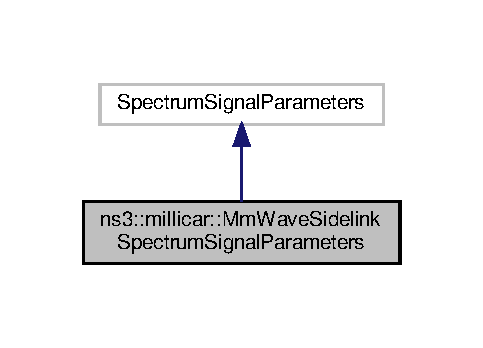
\includegraphics[width=232pt]{structns3_1_1millicar_1_1MmWaveSidelinkSpectrumSignalParameters__inherit__graph}
\end{center}
\end{figure}


Collaboration diagram for ns3\+:\+:millicar\+:\+:Mm\+Wave\+Sidelink\+Spectrum\+Signal\+Parameters\+:
\nopagebreak
\begin{figure}[H]
\begin{center}
\leavevmode
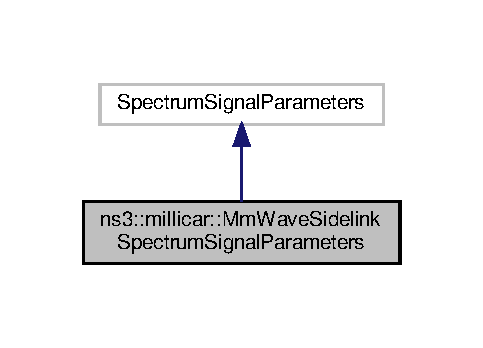
\includegraphics[width=232pt]{structns3_1_1millicar_1_1MmWaveSidelinkSpectrumSignalParameters__coll__graph}
\end{center}
\end{figure}
\subsection*{Public Member Functions}
\begin{DoxyCompactItemize}
\item 
\mbox{\Hypertarget{structns3_1_1millicar_1_1MmWaveSidelinkSpectrumSignalParameters_a16cf1f44f97b253aef602fe650dbe69e}\label{structns3_1_1millicar_1_1MmWaveSidelinkSpectrumSignalParameters_a16cf1f44f97b253aef602fe650dbe69e}} 
virtual Ptr$<$ Spectrum\+Signal\+Parameters $>$ {\bfseries Copy} ()
\item 
\hyperlink{structns3_1_1millicar_1_1MmWaveSidelinkSpectrumSignalParameters_ae23417b732d56ba404ddf098f21d264a}{Mm\+Wave\+Sidelink\+Spectrum\+Signal\+Parameters} ()
\item 
\hyperlink{structns3_1_1millicar_1_1MmWaveSidelinkSpectrumSignalParameters_ab40dd2c47c3058b56c99d671a4fd04cf}{Mm\+Wave\+Sidelink\+Spectrum\+Signal\+Parameters} (const \hyperlink{structns3_1_1millicar_1_1MmWaveSidelinkSpectrumSignalParameters}{Mm\+Wave\+Sidelink\+Spectrum\+Signal\+Parameters} \&p)
\end{DoxyCompactItemize}
\subsection*{Public Attributes}
\begin{DoxyCompactItemize}
\item 
\mbox{\Hypertarget{structns3_1_1millicar_1_1MmWaveSidelinkSpectrumSignalParameters_a873326282f3503a6bc088013ef75bced}\label{structns3_1_1millicar_1_1MmWaveSidelinkSpectrumSignalParameters_a873326282f3503a6bc088013ef75bced}} 
Ptr$<$ Packet\+Burst $>$ {\bfseries packet\+Burst}
\item 
\mbox{\Hypertarget{structns3_1_1millicar_1_1MmWaveSidelinkSpectrumSignalParameters_a5b489098e3e18ec32e05f5c50bc303d9}\label{structns3_1_1millicar_1_1MmWaveSidelinkSpectrumSignalParameters_a5b489098e3e18ec32e05f5c50bc303d9}} 
uint8\+\_\+t \hyperlink{structns3_1_1millicar_1_1MmWaveSidelinkSpectrumSignalParameters_a5b489098e3e18ec32e05f5c50bc303d9}{mcs}
\begin{DoxyCompactList}\small\item\em the modulation and coding scheme index to be used to transmit the transport block \end{DoxyCompactList}\item 
\mbox{\Hypertarget{structns3_1_1millicar_1_1MmWaveSidelinkSpectrumSignalParameters_abef1c09e8c217d564d7ab35c52776b9e}\label{structns3_1_1millicar_1_1MmWaveSidelinkSpectrumSignalParameters_abef1c09e8c217d564d7ab35c52776b9e}} 
uint8\+\_\+t \hyperlink{structns3_1_1millicar_1_1MmWaveSidelinkSpectrumSignalParameters_abef1c09e8c217d564d7ab35c52776b9e}{num\+Sym}
\begin{DoxyCompactList}\small\item\em the number of symbols associated to a specific transport block \end{DoxyCompactList}\item 
\mbox{\Hypertarget{structns3_1_1millicar_1_1MmWaveSidelinkSpectrumSignalParameters_a9f94a65733580e8fcec1b0d56c196004}\label{structns3_1_1millicar_1_1MmWaveSidelinkSpectrumSignalParameters_a9f94a65733580e8fcec1b0d56c196004}} 
uint16\+\_\+t \hyperlink{structns3_1_1millicar_1_1MmWaveSidelinkSpectrumSignalParameters_a9f94a65733580e8fcec1b0d56c196004}{sender\+Rnti}
\begin{DoxyCompactList}\small\item\em the R\+N\+TI which identifies the sender device \end{DoxyCompactList}\item 
\mbox{\Hypertarget{structns3_1_1millicar_1_1MmWaveSidelinkSpectrumSignalParameters_ac8ff697cac99b54d01a548783640c242}\label{structns3_1_1millicar_1_1MmWaveSidelinkSpectrumSignalParameters_ac8ff697cac99b54d01a548783640c242}} 
uint16\+\_\+t \hyperlink{structns3_1_1millicar_1_1MmWaveSidelinkSpectrumSignalParameters_ac8ff697cac99b54d01a548783640c242}{destination\+Rnti}
\begin{DoxyCompactList}\small\item\em the R\+N\+TI which identifies the destination device \end{DoxyCompactList}\item 
\mbox{\Hypertarget{structns3_1_1millicar_1_1MmWaveSidelinkSpectrumSignalParameters_ac95661f1e69b935be32dd73d26d5ada5}\label{structns3_1_1millicar_1_1MmWaveSidelinkSpectrumSignalParameters_ac95661f1e69b935be32dd73d26d5ada5}} 
uint32\+\_\+t \hyperlink{structns3_1_1millicar_1_1MmWaveSidelinkSpectrumSignalParameters_ac95661f1e69b935be32dd73d26d5ada5}{size}
\begin{DoxyCompactList}\small\item\em the size of the corresponding transport block \end{DoxyCompactList}\item 
\mbox{\Hypertarget{structns3_1_1millicar_1_1MmWaveSidelinkSpectrumSignalParameters_a38ff1054186e12389fa9003c46b20e18}\label{structns3_1_1millicar_1_1MmWaveSidelinkSpectrumSignalParameters_a38ff1054186e12389fa9003c46b20e18}} 
std\+::vector$<$ int $>$ \hyperlink{structns3_1_1millicar_1_1MmWaveSidelinkSpectrumSignalParameters_a38ff1054186e12389fa9003c46b20e18}{rb\+Bitmap}
\begin{DoxyCompactList}\small\item\em the resource blocks bitmap associated to the transport block \end{DoxyCompactList}\item 
\mbox{\Hypertarget{structns3_1_1millicar_1_1MmWaveSidelinkSpectrumSignalParameters_a15bd0c3e1ff3ab2fd3008eda2d242c23}\label{structns3_1_1millicar_1_1MmWaveSidelinkSpectrumSignalParameters_a15bd0c3e1ff3ab2fd3008eda2d242c23}} 
bool {\bfseries pss}
\end{DoxyCompactItemize}


\subsection{Constructor \& Destructor Documentation}
\mbox{\Hypertarget{structns3_1_1millicar_1_1MmWaveSidelinkSpectrumSignalParameters_ae23417b732d56ba404ddf098f21d264a}\label{structns3_1_1millicar_1_1MmWaveSidelinkSpectrumSignalParameters_ae23417b732d56ba404ddf098f21d264a}} 
\index{ns3\+::millicar\+::\+Mm\+Wave\+Sidelink\+Spectrum\+Signal\+Parameters@{ns3\+::millicar\+::\+Mm\+Wave\+Sidelink\+Spectrum\+Signal\+Parameters}!Mm\+Wave\+Sidelink\+Spectrum\+Signal\+Parameters@{Mm\+Wave\+Sidelink\+Spectrum\+Signal\+Parameters}}
\index{Mm\+Wave\+Sidelink\+Spectrum\+Signal\+Parameters@{Mm\+Wave\+Sidelink\+Spectrum\+Signal\+Parameters}!ns3\+::millicar\+::\+Mm\+Wave\+Sidelink\+Spectrum\+Signal\+Parameters@{ns3\+::millicar\+::\+Mm\+Wave\+Sidelink\+Spectrum\+Signal\+Parameters}}
\subsubsection{\texorpdfstring{Mm\+Wave\+Sidelink\+Spectrum\+Signal\+Parameters()}{MmWaveSidelinkSpectrumSignalParameters()}\hspace{0.1cm}{\footnotesize\ttfamily [1/2]}}
{\footnotesize\ttfamily ns3\+::millicar\+::\+Mm\+Wave\+Sidelink\+Spectrum\+Signal\+Parameters\+::\+Mm\+Wave\+Sidelink\+Spectrum\+Signal\+Parameters (\begin{DoxyParamCaption}{ }\end{DoxyParamCaption})}

default constructor \mbox{\Hypertarget{structns3_1_1millicar_1_1MmWaveSidelinkSpectrumSignalParameters_ab40dd2c47c3058b56c99d671a4fd04cf}\label{structns3_1_1millicar_1_1MmWaveSidelinkSpectrumSignalParameters_ab40dd2c47c3058b56c99d671a4fd04cf}} 
\index{ns3\+::millicar\+::\+Mm\+Wave\+Sidelink\+Spectrum\+Signal\+Parameters@{ns3\+::millicar\+::\+Mm\+Wave\+Sidelink\+Spectrum\+Signal\+Parameters}!Mm\+Wave\+Sidelink\+Spectrum\+Signal\+Parameters@{Mm\+Wave\+Sidelink\+Spectrum\+Signal\+Parameters}}
\index{Mm\+Wave\+Sidelink\+Spectrum\+Signal\+Parameters@{Mm\+Wave\+Sidelink\+Spectrum\+Signal\+Parameters}!ns3\+::millicar\+::\+Mm\+Wave\+Sidelink\+Spectrum\+Signal\+Parameters@{ns3\+::millicar\+::\+Mm\+Wave\+Sidelink\+Spectrum\+Signal\+Parameters}}
\subsubsection{\texorpdfstring{Mm\+Wave\+Sidelink\+Spectrum\+Signal\+Parameters()}{MmWaveSidelinkSpectrumSignalParameters()}\hspace{0.1cm}{\footnotesize\ttfamily [2/2]}}
{\footnotesize\ttfamily ns3\+::millicar\+::\+Mm\+Wave\+Sidelink\+Spectrum\+Signal\+Parameters\+::\+Mm\+Wave\+Sidelink\+Spectrum\+Signal\+Parameters (\begin{DoxyParamCaption}\item[{const \hyperlink{structns3_1_1millicar_1_1MmWaveSidelinkSpectrumSignalParameters}{Mm\+Wave\+Sidelink\+Spectrum\+Signal\+Parameters} \&}]{p }\end{DoxyParamCaption})}

copy constructor 

The documentation for this struct was generated from the following files\+:\begin{DoxyCompactItemize}
\item 
model/mmwave-\/sidelink-\/spectrum-\/signal-\/parameters.\+h\item 
model/mmwave-\/sidelink-\/spectrum-\/signal-\/parameters.\+cc\end{DoxyCompactItemize}

\hypertarget{classns3_1_1millicar_1_1MmWaveVehicularAntennaArrayModel}{}\section{ns3\+:\+:millicar\+:\+:Mm\+Wave\+Vehicular\+Antenna\+Array\+Model Class Reference}
\label{classns3_1_1millicar_1_1MmWaveVehicularAntennaArrayModel}\index{ns3\+::millicar\+::\+Mm\+Wave\+Vehicular\+Antenna\+Array\+Model@{ns3\+::millicar\+::\+Mm\+Wave\+Vehicular\+Antenna\+Array\+Model}}


Inheritance diagram for ns3\+:\+:millicar\+:\+:Mm\+Wave\+Vehicular\+Antenna\+Array\+Model\+:\nopagebreak
\begin{figure}[H]
\begin{center}
\leavevmode
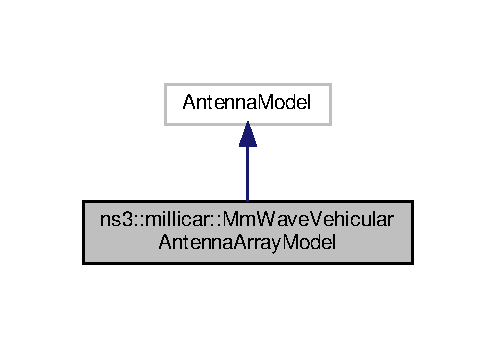
\includegraphics[width=238pt]{classns3_1_1millicar_1_1MmWaveVehicularAntennaArrayModel__inherit__graph}
\end{center}
\end{figure}


Collaboration diagram for ns3\+:\+:millicar\+:\+:Mm\+Wave\+Vehicular\+Antenna\+Array\+Model\+:\nopagebreak
\begin{figure}[H]
\begin{center}
\leavevmode
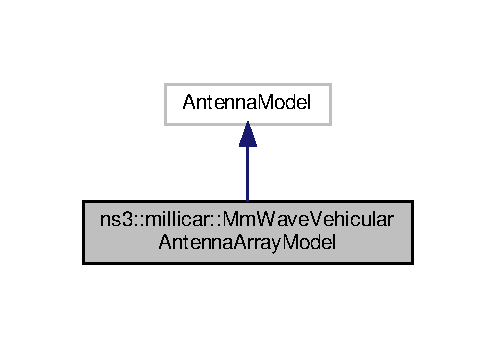
\includegraphics[width=238pt]{classns3_1_1millicar_1_1MmWaveVehicularAntennaArrayModel__coll__graph}
\end{center}
\end{figure}
\subsection*{Public Member Functions}
\begin{DoxyCompactItemize}
\item 
\mbox{\Hypertarget{classns3_1_1millicar_1_1MmWaveVehicularAntennaArrayModel_a9613fa40bea2b327c7f988d32c565011}\label{classns3_1_1millicar_1_1MmWaveVehicularAntennaArrayModel_a9613fa40bea2b327c7f988d32c565011}} 
virtual double {\bfseries Get\+Gain\+Db} (Angles a)
\item 
\mbox{\Hypertarget{classns3_1_1millicar_1_1MmWaveVehicularAntennaArrayModel_ae655e771ff32627633d3022dd5e9d2b0}\label{classns3_1_1millicar_1_1MmWaveVehicularAntennaArrayModel_ae655e771ff32627633d3022dd5e9d2b0}} 
void {\bfseries Set\+Beamforming\+Vector\+Panel} (complex\+Vector\+\_\+t antenna\+Weights, Ptr$<$ Net\+Device $>$ device=0)
\item 
\mbox{\Hypertarget{classns3_1_1millicar_1_1MmWaveVehicularAntennaArrayModel_a18cc7940ab4c2ff4792ff1190abdd31e}\label{classns3_1_1millicar_1_1MmWaveVehicularAntennaArrayModel_a18cc7940ab4c2ff4792ff1190abdd31e}} 
void {\bfseries Set\+Beamforming\+Vector\+With\+Delay} (complex\+Vector\+\_\+t antenna\+Weights, Ptr$<$ Net\+Device $>$ device=0)
\item 
\mbox{\Hypertarget{classns3_1_1millicar_1_1MmWaveVehicularAntennaArrayModel_a11638107e20004a64b705d065836efa4}\label{classns3_1_1millicar_1_1MmWaveVehicularAntennaArrayModel_a11638107e20004a64b705d065836efa4}} 
void {\bfseries Set\+Beamforming\+Vector\+Panel\+Devices} (Ptr$<$ Net\+Device $>$ this\+Device=0, Ptr$<$ Net\+Device $>$ other\+Device=0)
\item 
\mbox{\Hypertarget{classns3_1_1millicar_1_1MmWaveVehicularAntennaArrayModel_ab12886777ec5ad1263929feb384532ec}\label{classns3_1_1millicar_1_1MmWaveVehicularAntennaArrayModel_ab12886777ec5ad1263929feb384532ec}} 
void {\bfseries Change\+Beamforming\+Vector\+Panel} (Ptr$<$ Net\+Device $>$ device)
\item 
\mbox{\Hypertarget{classns3_1_1millicar_1_1MmWaveVehicularAntennaArrayModel_aba8ce056f2e0df98d2ba75980ff0af7e}\label{classns3_1_1millicar_1_1MmWaveVehicularAntennaArrayModel_aba8ce056f2e0df98d2ba75980ff0af7e}} 
complex\+Vector\+\_\+t {\bfseries Get\+Beamforming\+Vector\+Panel} ()
\item 
\mbox{\Hypertarget{classns3_1_1millicar_1_1MmWaveVehicularAntennaArrayModel_abb1c4f0625fd0568b3b493f3ffe4dd04}\label{classns3_1_1millicar_1_1MmWaveVehicularAntennaArrayModel_abb1c4f0625fd0568b3b493f3ffe4dd04}} 
complex\+Vector\+\_\+t {\bfseries Get\+Beamforming\+Vector\+Panel} (Ptr$<$ Net\+Device $>$ device)
\item 
\mbox{\Hypertarget{classns3_1_1millicar_1_1MmWaveVehicularAntennaArrayModel_a521d963c3c113ad294783042630a727a}\label{classns3_1_1millicar_1_1MmWaveVehicularAntennaArrayModel_a521d963c3c113ad294783042630a727a}} 
void {\bfseries Change\+To\+Omni\+Tx} ()
\item 
\mbox{\Hypertarget{classns3_1_1millicar_1_1MmWaveVehicularAntennaArrayModel_af8dd71912feca69c61de21b73a48864c}\label{classns3_1_1millicar_1_1MmWaveVehicularAntennaArrayModel_af8dd71912feca69c61de21b73a48864c}} 
bool {\bfseries Is\+Omni\+Tx} ()
\item 
\mbox{\Hypertarget{classns3_1_1millicar_1_1MmWaveVehicularAntennaArrayModel_a5d18fb70c35545e3fb6ceab7cdfbf29f}\label{classns3_1_1millicar_1_1MmWaveVehicularAntennaArrayModel_a5d18fb70c35545e3fb6ceab7cdfbf29f}} 
double {\bfseries Get\+Radiation\+Pattern} (double vangle, double hangle=0)
\item 
\mbox{\Hypertarget{classns3_1_1millicar_1_1MmWaveVehicularAntennaArrayModel_ac56f86f72c7f92e13cc846f803c53f0c}\label{classns3_1_1millicar_1_1MmWaveVehicularAntennaArrayModel_ac56f86f72c7f92e13cc846f803c53f0c}} 
Vector {\bfseries Get\+Antenna\+Location} (uint16\+\_\+t index, uint16\+\_\+t $\ast$antenna\+Num)
\item 
\mbox{\Hypertarget{classns3_1_1millicar_1_1MmWaveVehicularAntennaArrayModel_a18cb8824e341b7d80d1fd9a011604a8d}\label{classns3_1_1millicar_1_1MmWaveVehicularAntennaArrayModel_a18cb8824e341b7d80d1fd9a011604a8d}} 
void {\bfseries Set\+Sector} (uint8\+\_\+t sector, uint16\+\_\+t $\ast$antenna\+Num, double elevation=90)
\item 
\mbox{\Hypertarget{classns3_1_1millicar_1_1MmWaveVehicularAntennaArrayModel_aad67935b04563306cbb4e28fcd075758}\label{classns3_1_1millicar_1_1MmWaveVehicularAntennaArrayModel_aad67935b04563306cbb4e28fcd075758}} 
void {\bfseries Set\+Planes\+Number} (uint8\+\_\+t planes\+Number)
\item 
\mbox{\Hypertarget{classns3_1_1millicar_1_1MmWaveVehicularAntennaArrayModel_ad45087d492c9127b7d2113c6866b40b6}\label{classns3_1_1millicar_1_1MmWaveVehicularAntennaArrayModel_ad45087d492c9127b7d2113c6866b40b6}} 
double {\bfseries Get\+Planes\+Id} (void)
\item 
\mbox{\Hypertarget{classns3_1_1millicar_1_1MmWaveVehicularAntennaArrayModel_adb3a2e826cde719d7cc32b23bafeee98}\label{classns3_1_1millicar_1_1MmWaveVehicularAntennaArrayModel_adb3a2e826cde719d7cc32b23bafeee98}} 
void {\bfseries Set\+Device\+Type} (bool is\+Ue)
\item 
\mbox{\Hypertarget{classns3_1_1millicar_1_1MmWaveVehicularAntennaArrayModel_aa570481367e2f3677f1ea4eedd37be40}\label{classns3_1_1millicar_1_1MmWaveVehicularAntennaArrayModel_aa570481367e2f3677f1ea4eedd37be40}} 
void {\bfseries Set\+Tot\+No\+Array\+Elements} (uint64\+\_\+t array\+Elements)
\item 
\mbox{\Hypertarget{classns3_1_1millicar_1_1MmWaveVehicularAntennaArrayModel_a673379bcc08edd4e4a5087cc98bde535}\label{classns3_1_1millicar_1_1MmWaveVehicularAntennaArrayModel_a673379bcc08edd4e4a5087cc98bde535}} 
uint64\+\_\+t {\bfseries Get\+Tot\+No\+Array\+Elements} () const
\item 
\mbox{\Hypertarget{classns3_1_1millicar_1_1MmWaveVehicularAntennaArrayModel_ab7fca5cec95fb67796031fa56d15f737}\label{classns3_1_1millicar_1_1MmWaveVehicularAntennaArrayModel_ab7fca5cec95fb67796031fa56d15f737}} 
double {\bfseries Get\+Offset} ()
\item 
\mbox{\Hypertarget{classns3_1_1millicar_1_1MmWaveVehicularAntennaArrayModel_a92eee4f359b18cb6b5a7d472fe53dfe9}\label{classns3_1_1millicar_1_1MmWaveVehicularAntennaArrayModel_a92eee4f359b18cb6b5a7d472fe53dfe9}} 
Ptr$<$ Net\+Device $>$ {\bfseries Get\+Current\+Device} ()
\item 
\mbox{\Hypertarget{classns3_1_1millicar_1_1MmWaveVehicularAntennaArrayModel_aa4665c98fbc53852782e954baf1e4919}\label{classns3_1_1millicar_1_1MmWaveVehicularAntennaArrayModel_aa4665c98fbc53852782e954baf1e4919}} 
Time {\bfseries Get\+Last\+Update} (Ptr$<$ Net\+Device $>$ device)
\end{DoxyCompactItemize}
\subsection*{Static Public Member Functions}
\begin{DoxyCompactItemize}
\item 
\mbox{\Hypertarget{classns3_1_1millicar_1_1MmWaveVehicularAntennaArrayModel_a450465ae8a280813c5d29d53a57cb590}\label{classns3_1_1millicar_1_1MmWaveVehicularAntennaArrayModel_a450465ae8a280813c5d29d53a57cb590}} 
static Type\+Id {\bfseries Get\+Type\+Id} ()
\end{DoxyCompactItemize}


The documentation for this class was generated from the following files\+:\begin{DoxyCompactItemize}
\item 
model/mmwave-\/vehicular-\/antenna-\/array-\/model.\+h\item 
model/mmwave-\/vehicular-\/antenna-\/array-\/model.\+cc\end{DoxyCompactItemize}

\hypertarget{classns3_1_1millicar_1_1MmWaveVehicularHelper}{}\section{ns3\+:\+:millicar\+:\+:Mm\+Wave\+Vehicular\+Helper Class Reference}
\label{classns3_1_1millicar_1_1MmWaveVehicularHelper}\index{ns3\+::millicar\+::\+Mm\+Wave\+Vehicular\+Helper@{ns3\+::millicar\+::\+Mm\+Wave\+Vehicular\+Helper}}


{\ttfamily \#include $<$mmwave-\/vehicular-\/helper.\+h$>$}



Inheritance diagram for ns3\+:\+:millicar\+:\+:Mm\+Wave\+Vehicular\+Helper\+:
\nopagebreak
\begin{figure}[H]
\begin{center}
\leavevmode
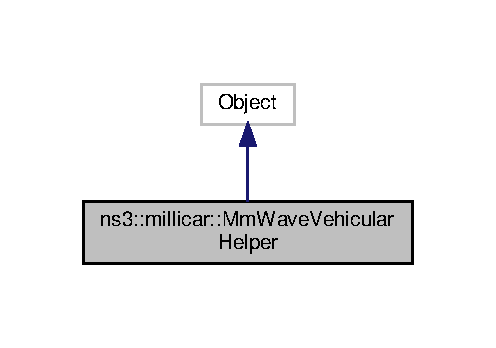
\includegraphics[width=238pt]{classns3_1_1millicar_1_1MmWaveVehicularHelper__inherit__graph}
\end{center}
\end{figure}


Collaboration diagram for ns3\+:\+:millicar\+:\+:Mm\+Wave\+Vehicular\+Helper\+:
\nopagebreak
\begin{figure}[H]
\begin{center}
\leavevmode
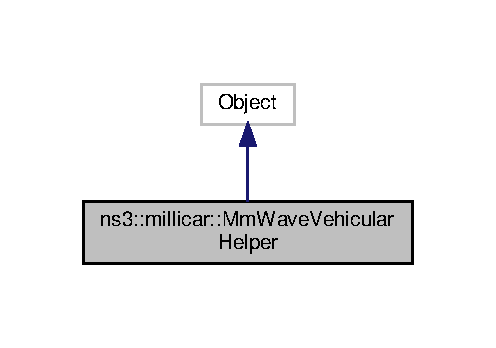
\includegraphics[width=238pt]{classns3_1_1millicar_1_1MmWaveVehicularHelper__coll__graph}
\end{center}
\end{figure}
\subsection*{Public Types}
\begin{DoxyCompactItemize}
\item 
enum \hyperlink{classns3_1_1millicar_1_1MmWaveVehicularHelper_a7b56a1dec16b395a2b07f3e2267bc8e8}{Scheduling\+Pattern\+Option\+\_\+t} \{ {\bfseries D\+E\+F\+A\+U\+LT} = 1, 
{\bfseries O\+P\+T\+I\+M\+I\+Z\+ED} = 2
 \}
\end{DoxyCompactItemize}
\subsection*{Public Member Functions}
\begin{DoxyCompactItemize}
\item 
\hyperlink{classns3_1_1millicar_1_1MmWaveVehicularHelper_aba839ec88d07cfaf576bb7c69cbdfa43}{Mm\+Wave\+Vehicular\+Helper} (void)
\item 
virtual \hyperlink{classns3_1_1millicar_1_1MmWaveVehicularHelper_ae49877d6086c33c972893422dd242bd4}{$\sim$\+Mm\+Wave\+Vehicular\+Helper} (void)
\item 
Net\+Device\+Container \hyperlink{classns3_1_1millicar_1_1MmWaveVehicularHelper_adb23c9d4f13972fd3bac3b35a23582c4}{Install\+Mm\+Wave\+Vehicular\+Net\+Devices} (Node\+Container nodes)
\item 
void \hyperlink{classns3_1_1millicar_1_1MmWaveVehicularHelper_a0976a2d0e5f3bce4bc7fb75f67209d8f}{Set\+Configuration\+Parameters} (Ptr$<$ mmwave\+::\+Mm\+Wave\+Phy\+Mac\+Common $>$ conf)
\item 
Ptr$<$ mmwave\+::\+Mm\+Wave\+Phy\+Mac\+Common $>$ \hyperlink{classns3_1_1millicar_1_1MmWaveVehicularHelper_aa1ab3205ac126fabac48608c0bbf8dcd}{Get\+Configuration\+Parameters} () const
\item 
void \hyperlink{classns3_1_1millicar_1_1MmWaveVehicularHelper_a0bd9a7da6f128d5cf4411e8757d9c884}{Set\+Propagation\+Loss\+Model\+Type} (std\+::string plm)
\item 
void \hyperlink{classns3_1_1millicar_1_1MmWaveVehicularHelper_ae03289dc88f603994c8ec5649756878f}{Set\+Spectrum\+Propagation\+Loss\+Model\+Type} (std\+::string splm)
\item 
void \hyperlink{classns3_1_1millicar_1_1MmWaveVehicularHelper_a065bd56895c9de5e3df2e8e733a29f3b}{Set\+Propagation\+Delay\+Model\+Type} (std\+::string pdm)
\item 
void \hyperlink{classns3_1_1millicar_1_1MmWaveVehicularHelper_ad534c932d9a9ff86e41fa6f09377001f}{Pair\+Devices} (Net\+Device\+Container devices)
\item 
void \hyperlink{classns3_1_1millicar_1_1MmWaveVehicularHelper_a8653a3225aa1df7ef17eb9ed3d6ebab9}{Set\+Numerology} (uint8\+\_\+t index)
\item 
std\+::vector$<$ uint16\+\_\+t $>$ \hyperlink{classns3_1_1millicar_1_1MmWaveVehicularHelper_a6bc119194b9aa09c56d9f9e529e2e09a}{Create\+Scheduling\+Pattern} (Net\+Device\+Container devices)
\item 
void \hyperlink{classns3_1_1millicar_1_1MmWaveVehicularHelper_a909144ad73428efd96a27612757ec08a}{Set\+Scheduling\+Pattern\+Option\+Type} (\hyperlink{classns3_1_1millicar_1_1MmWaveVehicularHelper_a7b56a1dec16b395a2b07f3e2267bc8e8}{Scheduling\+Pattern\+Option\+\_\+t} spo)
\item 
\hyperlink{classns3_1_1millicar_1_1MmWaveVehicularHelper_a7b56a1dec16b395a2b07f3e2267bc8e8}{Scheduling\+Pattern\+Option\+\_\+t} \hyperlink{classns3_1_1millicar_1_1MmWaveVehicularHelper_a6d6431806df6b60f555880c26c21ce5e}{Get\+Scheduling\+Pattern\+Option\+Type} () const
\end{DoxyCompactItemize}
\subsection*{Static Public Member Functions}
\begin{DoxyCompactItemize}
\item 
\mbox{\Hypertarget{classns3_1_1millicar_1_1MmWaveVehicularHelper_a281b5ef7548fe7c8a67b3deaaba28a29}\label{classns3_1_1millicar_1_1MmWaveVehicularHelper_a281b5ef7548fe7c8a67b3deaaba28a29}} 
static Type\+Id {\bfseries Get\+Type\+Id} (void)
\end{DoxyCompactItemize}
\subsection*{Protected Member Functions}
\begin{DoxyCompactItemize}
\item 
\mbox{\Hypertarget{classns3_1_1millicar_1_1MmWaveVehicularHelper_a606e9f24b4aee9d8e77cf476827dabf8}\label{classns3_1_1millicar_1_1MmWaveVehicularHelper_a606e9f24b4aee9d8e77cf476827dabf8}} 
virtual void {\bfseries Do\+Initialize} (void) override
\end{DoxyCompactItemize}


\subsection{Detailed Description}
This class is used for the creation of Mm\+Wave\+Vehicular\+Net\+Devices and their configuration 

\subsection{Member Enumeration Documentation}
\mbox{\Hypertarget{classns3_1_1millicar_1_1MmWaveVehicularHelper_a7b56a1dec16b395a2b07f3e2267bc8e8}\label{classns3_1_1millicar_1_1MmWaveVehicularHelper_a7b56a1dec16b395a2b07f3e2267bc8e8}} 
\index{ns3\+::millicar\+::\+Mm\+Wave\+Vehicular\+Helper@{ns3\+::millicar\+::\+Mm\+Wave\+Vehicular\+Helper}!Scheduling\+Pattern\+Option\+\_\+t@{Scheduling\+Pattern\+Option\+\_\+t}}
\index{Scheduling\+Pattern\+Option\+\_\+t@{Scheduling\+Pattern\+Option\+\_\+t}!ns3\+::millicar\+::\+Mm\+Wave\+Vehicular\+Helper@{ns3\+::millicar\+::\+Mm\+Wave\+Vehicular\+Helper}}
\subsubsection{\texorpdfstring{Scheduling\+Pattern\+Option\+\_\+t}{SchedulingPatternOption\_t}}
{\footnotesize\ttfamily enum \hyperlink{classns3_1_1millicar_1_1MmWaveVehicularHelper_a7b56a1dec16b395a2b07f3e2267bc8e8}{ns3\+::millicar\+::\+Mm\+Wave\+Vehicular\+Helper\+::\+Scheduling\+Pattern\+Option\+\_\+t}}

Identifies the supported scheduling pattern policies 

\subsection{Constructor \& Destructor Documentation}
\mbox{\Hypertarget{classns3_1_1millicar_1_1MmWaveVehicularHelper_aba839ec88d07cfaf576bb7c69cbdfa43}\label{classns3_1_1millicar_1_1MmWaveVehicularHelper_aba839ec88d07cfaf576bb7c69cbdfa43}} 
\index{ns3\+::millicar\+::\+Mm\+Wave\+Vehicular\+Helper@{ns3\+::millicar\+::\+Mm\+Wave\+Vehicular\+Helper}!Mm\+Wave\+Vehicular\+Helper@{Mm\+Wave\+Vehicular\+Helper}}
\index{Mm\+Wave\+Vehicular\+Helper@{Mm\+Wave\+Vehicular\+Helper}!ns3\+::millicar\+::\+Mm\+Wave\+Vehicular\+Helper@{ns3\+::millicar\+::\+Mm\+Wave\+Vehicular\+Helper}}
\subsubsection{\texorpdfstring{Mm\+Wave\+Vehicular\+Helper()}{MmWaveVehicularHelper()}}
{\footnotesize\ttfamily ns3\+::millicar\+::\+Mm\+Wave\+Vehicular\+Helper\+::\+Mm\+Wave\+Vehicular\+Helper (\begin{DoxyParamCaption}\item[{void}]{ }\end{DoxyParamCaption})}

Constructor \mbox{\Hypertarget{classns3_1_1millicar_1_1MmWaveVehicularHelper_ae49877d6086c33c972893422dd242bd4}\label{classns3_1_1millicar_1_1MmWaveVehicularHelper_ae49877d6086c33c972893422dd242bd4}} 
\index{ns3\+::millicar\+::\+Mm\+Wave\+Vehicular\+Helper@{ns3\+::millicar\+::\+Mm\+Wave\+Vehicular\+Helper}!````~Mm\+Wave\+Vehicular\+Helper@{$\sim$\+Mm\+Wave\+Vehicular\+Helper}}
\index{````~Mm\+Wave\+Vehicular\+Helper@{$\sim$\+Mm\+Wave\+Vehicular\+Helper}!ns3\+::millicar\+::\+Mm\+Wave\+Vehicular\+Helper@{ns3\+::millicar\+::\+Mm\+Wave\+Vehicular\+Helper}}
\subsubsection{\texorpdfstring{$\sim$\+Mm\+Wave\+Vehicular\+Helper()}{~MmWaveVehicularHelper()}}
{\footnotesize\ttfamily ns3\+::millicar\+::\+Mm\+Wave\+Vehicular\+Helper\+::$\sim$\+Mm\+Wave\+Vehicular\+Helper (\begin{DoxyParamCaption}\item[{void}]{ }\end{DoxyParamCaption})\hspace{0.3cm}{\ttfamily [virtual]}}

Destructor 

\subsection{Member Function Documentation}
\mbox{\Hypertarget{classns3_1_1millicar_1_1MmWaveVehicularHelper_a6bc119194b9aa09c56d9f9e529e2e09a}\label{classns3_1_1millicar_1_1MmWaveVehicularHelper_a6bc119194b9aa09c56d9f9e529e2e09a}} 
\index{ns3\+::millicar\+::\+Mm\+Wave\+Vehicular\+Helper@{ns3\+::millicar\+::\+Mm\+Wave\+Vehicular\+Helper}!Create\+Scheduling\+Pattern@{Create\+Scheduling\+Pattern}}
\index{Create\+Scheduling\+Pattern@{Create\+Scheduling\+Pattern}!ns3\+::millicar\+::\+Mm\+Wave\+Vehicular\+Helper@{ns3\+::millicar\+::\+Mm\+Wave\+Vehicular\+Helper}}
\subsubsection{\texorpdfstring{Create\+Scheduling\+Pattern()}{CreateSchedulingPattern()}}
{\footnotesize\ttfamily std\+::vector$<$ uint16\+\_\+t $>$ ns3\+::millicar\+::\+Mm\+Wave\+Vehicular\+Helper\+::\+Create\+Scheduling\+Pattern (\begin{DoxyParamCaption}\item[{Net\+Device\+Container}]{devices }\end{DoxyParamCaption})}

Configure the scheduling pattern for a specific group of devices 
\begin{DoxyParams}{Parameters}
{\em devices} & the Net\+Device\+Container with the devices \\
\hline
\end{DoxyParams}
\begin{DoxyReturn}{Returns}
a vector of integers representing the scheduling pattern 
\end{DoxyReturn}
\mbox{\Hypertarget{classns3_1_1millicar_1_1MmWaveVehicularHelper_aa1ab3205ac126fabac48608c0bbf8dcd}\label{classns3_1_1millicar_1_1MmWaveVehicularHelper_aa1ab3205ac126fabac48608c0bbf8dcd}} 
\index{ns3\+::millicar\+::\+Mm\+Wave\+Vehicular\+Helper@{ns3\+::millicar\+::\+Mm\+Wave\+Vehicular\+Helper}!Get\+Configuration\+Parameters@{Get\+Configuration\+Parameters}}
\index{Get\+Configuration\+Parameters@{Get\+Configuration\+Parameters}!ns3\+::millicar\+::\+Mm\+Wave\+Vehicular\+Helper@{ns3\+::millicar\+::\+Mm\+Wave\+Vehicular\+Helper}}
\subsubsection{\texorpdfstring{Get\+Configuration\+Parameters()}{GetConfigurationParameters()}}
{\footnotesize\ttfamily Ptr$<$ mmwave\+::\+Mm\+Wave\+Phy\+Mac\+Common $>$ ns3\+::millicar\+::\+Mm\+Wave\+Vehicular\+Helper\+::\+Get\+Configuration\+Parameters (\begin{DoxyParamCaption}{ }\end{DoxyParamCaption}) const}

Retrieve pointer to the object that lists all the configuration parameters \begin{DoxyReturn}{Returns}
a pointer to a Mm\+Wave\+Phy\+Mac\+Common object 
\end{DoxyReturn}
\mbox{\Hypertarget{classns3_1_1millicar_1_1MmWaveVehicularHelper_a6d6431806df6b60f555880c26c21ce5e}\label{classns3_1_1millicar_1_1MmWaveVehicularHelper_a6d6431806df6b60f555880c26c21ce5e}} 
\index{ns3\+::millicar\+::\+Mm\+Wave\+Vehicular\+Helper@{ns3\+::millicar\+::\+Mm\+Wave\+Vehicular\+Helper}!Get\+Scheduling\+Pattern\+Option\+Type@{Get\+Scheduling\+Pattern\+Option\+Type}}
\index{Get\+Scheduling\+Pattern\+Option\+Type@{Get\+Scheduling\+Pattern\+Option\+Type}!ns3\+::millicar\+::\+Mm\+Wave\+Vehicular\+Helper@{ns3\+::millicar\+::\+Mm\+Wave\+Vehicular\+Helper}}
\subsubsection{\texorpdfstring{Get\+Scheduling\+Pattern\+Option\+Type()}{GetSchedulingPatternOptionType()}}
{\footnotesize\ttfamily \hyperlink{classns3_1_1millicar_1_1MmWaveVehicularHelper_a7b56a1dec16b395a2b07f3e2267bc8e8}{Mm\+Wave\+Vehicular\+Helper\+::\+Scheduling\+Pattern\+Option\+\_\+t} ns3\+::millicar\+::\+Mm\+Wave\+Vehicular\+Helper\+::\+Get\+Scheduling\+Pattern\+Option\+Type (\begin{DoxyParamCaption}{ }\end{DoxyParamCaption}) const}

Returns the adopted scheduling pattern policy \begin{DoxyReturn}{Returns}
the adopted scheduling pattern policy 
\end{DoxyReturn}
\mbox{\Hypertarget{classns3_1_1millicar_1_1MmWaveVehicularHelper_adb23c9d4f13972fd3bac3b35a23582c4}\label{classns3_1_1millicar_1_1MmWaveVehicularHelper_adb23c9d4f13972fd3bac3b35a23582c4}} 
\index{ns3\+::millicar\+::\+Mm\+Wave\+Vehicular\+Helper@{ns3\+::millicar\+::\+Mm\+Wave\+Vehicular\+Helper}!Install\+Mm\+Wave\+Vehicular\+Net\+Devices@{Install\+Mm\+Wave\+Vehicular\+Net\+Devices}}
\index{Install\+Mm\+Wave\+Vehicular\+Net\+Devices@{Install\+Mm\+Wave\+Vehicular\+Net\+Devices}!ns3\+::millicar\+::\+Mm\+Wave\+Vehicular\+Helper@{ns3\+::millicar\+::\+Mm\+Wave\+Vehicular\+Helper}}
\subsubsection{\texorpdfstring{Install\+Mm\+Wave\+Vehicular\+Net\+Devices()}{InstallMmWaveVehicularNetDevices()}}
{\footnotesize\ttfamily Net\+Device\+Container ns3\+::millicar\+::\+Mm\+Wave\+Vehicular\+Helper\+::\+Install\+Mm\+Wave\+Vehicular\+Net\+Devices (\begin{DoxyParamCaption}\item[{Node\+Container}]{nodes }\end{DoxyParamCaption})}

Install a \hyperlink{classns3_1_1millicar_1_1MmWaveVehicularNetDevice}{Mm\+Wave\+Vehicular\+Net\+Device} on each node in the container 
\begin{DoxyParams}{Parameters}
{\em nodes} & the node container \\
\hline
\end{DoxyParams}
\begin{DoxyReturn}{Returns}
a Net\+Device\+Container containing the installed devices 
\end{DoxyReturn}
\mbox{\Hypertarget{classns3_1_1millicar_1_1MmWaveVehicularHelper_ad534c932d9a9ff86e41fa6f09377001f}\label{classns3_1_1millicar_1_1MmWaveVehicularHelper_ad534c932d9a9ff86e41fa6f09377001f}} 
\index{ns3\+::millicar\+::\+Mm\+Wave\+Vehicular\+Helper@{ns3\+::millicar\+::\+Mm\+Wave\+Vehicular\+Helper}!Pair\+Devices@{Pair\+Devices}}
\index{Pair\+Devices@{Pair\+Devices}!ns3\+::millicar\+::\+Mm\+Wave\+Vehicular\+Helper@{ns3\+::millicar\+::\+Mm\+Wave\+Vehicular\+Helper}}
\subsubsection{\texorpdfstring{Pair\+Devices()}{PairDevices()}}
{\footnotesize\ttfamily void ns3\+::millicar\+::\+Mm\+Wave\+Vehicular\+Helper\+::\+Pair\+Devices (\begin{DoxyParamCaption}\item[{Net\+Device\+Container}]{devices }\end{DoxyParamCaption})}

Associate the devices in the container 
\begin{DoxyParams}{Parameters}
{\em devices} & the Net\+Device\+Container with the devices \\
\hline
\end{DoxyParams}
\mbox{\Hypertarget{classns3_1_1millicar_1_1MmWaveVehicularHelper_a0976a2d0e5f3bce4bc7fb75f67209d8f}\label{classns3_1_1millicar_1_1MmWaveVehicularHelper_a0976a2d0e5f3bce4bc7fb75f67209d8f}} 
\index{ns3\+::millicar\+::\+Mm\+Wave\+Vehicular\+Helper@{ns3\+::millicar\+::\+Mm\+Wave\+Vehicular\+Helper}!Set\+Configuration\+Parameters@{Set\+Configuration\+Parameters}}
\index{Set\+Configuration\+Parameters@{Set\+Configuration\+Parameters}!ns3\+::millicar\+::\+Mm\+Wave\+Vehicular\+Helper@{ns3\+::millicar\+::\+Mm\+Wave\+Vehicular\+Helper}}
\subsubsection{\texorpdfstring{Set\+Configuration\+Parameters()}{SetConfigurationParameters()}}
{\footnotesize\ttfamily void ns3\+::millicar\+::\+Mm\+Wave\+Vehicular\+Helper\+::\+Set\+Configuration\+Parameters (\begin{DoxyParamCaption}\item[{Ptr$<$ mmwave\+::\+Mm\+Wave\+Phy\+Mac\+Common $>$}]{conf }\end{DoxyParamCaption})}

Set the configuration parameters 
\begin{DoxyParams}{Parameters}
{\em conf} & pointer to mmwave\+::\+Mm\+Wave\+Phy\+Mac\+Common \\
\hline
\end{DoxyParams}
\mbox{\Hypertarget{classns3_1_1millicar_1_1MmWaveVehicularHelper_a8653a3225aa1df7ef17eb9ed3d6ebab9}\label{classns3_1_1millicar_1_1MmWaveVehicularHelper_a8653a3225aa1df7ef17eb9ed3d6ebab9}} 
\index{ns3\+::millicar\+::\+Mm\+Wave\+Vehicular\+Helper@{ns3\+::millicar\+::\+Mm\+Wave\+Vehicular\+Helper}!Set\+Numerology@{Set\+Numerology}}
\index{Set\+Numerology@{Set\+Numerology}!ns3\+::millicar\+::\+Mm\+Wave\+Vehicular\+Helper@{ns3\+::millicar\+::\+Mm\+Wave\+Vehicular\+Helper}}
\subsubsection{\texorpdfstring{Set\+Numerology()}{SetNumerology()}}
{\footnotesize\ttfamily void ns3\+::millicar\+::\+Mm\+Wave\+Vehicular\+Helper\+::\+Set\+Numerology (\begin{DoxyParamCaption}\item[{uint8\+\_\+t}]{index }\end{DoxyParamCaption})}

Configure the numerology index 
\begin{DoxyParams}{Parameters}
{\em index} & numerology index, used to define P\+HY layer parameters \\
\hline
\end{DoxyParams}
\mbox{\Hypertarget{classns3_1_1millicar_1_1MmWaveVehicularHelper_a065bd56895c9de5e3df2e8e733a29f3b}\label{classns3_1_1millicar_1_1MmWaveVehicularHelper_a065bd56895c9de5e3df2e8e733a29f3b}} 
\index{ns3\+::millicar\+::\+Mm\+Wave\+Vehicular\+Helper@{ns3\+::millicar\+::\+Mm\+Wave\+Vehicular\+Helper}!Set\+Propagation\+Delay\+Model\+Type@{Set\+Propagation\+Delay\+Model\+Type}}
\index{Set\+Propagation\+Delay\+Model\+Type@{Set\+Propagation\+Delay\+Model\+Type}!ns3\+::millicar\+::\+Mm\+Wave\+Vehicular\+Helper@{ns3\+::millicar\+::\+Mm\+Wave\+Vehicular\+Helper}}
\subsubsection{\texorpdfstring{Set\+Propagation\+Delay\+Model\+Type()}{SetPropagationDelayModelType()}}
{\footnotesize\ttfamily void ns3\+::millicar\+::\+Mm\+Wave\+Vehicular\+Helper\+::\+Set\+Propagation\+Delay\+Model\+Type (\begin{DoxyParamCaption}\item[{std\+::string}]{pdm }\end{DoxyParamCaption})}

Set the propagation delay model type 
\begin{DoxyParams}{Parameters}
{\em pdm} & the type id of the propagation delay model to use \\
\hline
\end{DoxyParams}
\mbox{\Hypertarget{classns3_1_1millicar_1_1MmWaveVehicularHelper_a0bd9a7da6f128d5cf4411e8757d9c884}\label{classns3_1_1millicar_1_1MmWaveVehicularHelper_a0bd9a7da6f128d5cf4411e8757d9c884}} 
\index{ns3\+::millicar\+::\+Mm\+Wave\+Vehicular\+Helper@{ns3\+::millicar\+::\+Mm\+Wave\+Vehicular\+Helper}!Set\+Propagation\+Loss\+Model\+Type@{Set\+Propagation\+Loss\+Model\+Type}}
\index{Set\+Propagation\+Loss\+Model\+Type@{Set\+Propagation\+Loss\+Model\+Type}!ns3\+::millicar\+::\+Mm\+Wave\+Vehicular\+Helper@{ns3\+::millicar\+::\+Mm\+Wave\+Vehicular\+Helper}}
\subsubsection{\texorpdfstring{Set\+Propagation\+Loss\+Model\+Type()}{SetPropagationLossModelType()}}
{\footnotesize\ttfamily void ns3\+::millicar\+::\+Mm\+Wave\+Vehicular\+Helper\+::\+Set\+Propagation\+Loss\+Model\+Type (\begin{DoxyParamCaption}\item[{std\+::string}]{plm }\end{DoxyParamCaption})}

Set the propagation loss model type 
\begin{DoxyParams}{Parameters}
{\em plm} & the type id of the propagation loss model to use \\
\hline
\end{DoxyParams}
\mbox{\Hypertarget{classns3_1_1millicar_1_1MmWaveVehicularHelper_a909144ad73428efd96a27612757ec08a}\label{classns3_1_1millicar_1_1MmWaveVehicularHelper_a909144ad73428efd96a27612757ec08a}} 
\index{ns3\+::millicar\+::\+Mm\+Wave\+Vehicular\+Helper@{ns3\+::millicar\+::\+Mm\+Wave\+Vehicular\+Helper}!Set\+Scheduling\+Pattern\+Option\+Type@{Set\+Scheduling\+Pattern\+Option\+Type}}
\index{Set\+Scheduling\+Pattern\+Option\+Type@{Set\+Scheduling\+Pattern\+Option\+Type}!ns3\+::millicar\+::\+Mm\+Wave\+Vehicular\+Helper@{ns3\+::millicar\+::\+Mm\+Wave\+Vehicular\+Helper}}
\subsubsection{\texorpdfstring{Set\+Scheduling\+Pattern\+Option\+Type()}{SetSchedulingPatternOptionType()}}
{\footnotesize\ttfamily void ns3\+::millicar\+::\+Mm\+Wave\+Vehicular\+Helper\+::\+Set\+Scheduling\+Pattern\+Option\+Type (\begin{DoxyParamCaption}\item[{\hyperlink{classns3_1_1millicar_1_1MmWaveVehicularHelper_a7b56a1dec16b395a2b07f3e2267bc8e8}{Scheduling\+Pattern\+Option\+\_\+t}}]{spo }\end{DoxyParamCaption})}

Set the scheduling pattern option type 
\begin{DoxyParams}{Parameters}
{\em spo} & the enum representing the scheduling pattern policy to be adopted \\
\hline
\end{DoxyParams}
\mbox{\Hypertarget{classns3_1_1millicar_1_1MmWaveVehicularHelper_ae03289dc88f603994c8ec5649756878f}\label{classns3_1_1millicar_1_1MmWaveVehicularHelper_ae03289dc88f603994c8ec5649756878f}} 
\index{ns3\+::millicar\+::\+Mm\+Wave\+Vehicular\+Helper@{ns3\+::millicar\+::\+Mm\+Wave\+Vehicular\+Helper}!Set\+Spectrum\+Propagation\+Loss\+Model\+Type@{Set\+Spectrum\+Propagation\+Loss\+Model\+Type}}
\index{Set\+Spectrum\+Propagation\+Loss\+Model\+Type@{Set\+Spectrum\+Propagation\+Loss\+Model\+Type}!ns3\+::millicar\+::\+Mm\+Wave\+Vehicular\+Helper@{ns3\+::millicar\+::\+Mm\+Wave\+Vehicular\+Helper}}
\subsubsection{\texorpdfstring{Set\+Spectrum\+Propagation\+Loss\+Model\+Type()}{SetSpectrumPropagationLossModelType()}}
{\footnotesize\ttfamily void ns3\+::millicar\+::\+Mm\+Wave\+Vehicular\+Helper\+::\+Set\+Spectrum\+Propagation\+Loss\+Model\+Type (\begin{DoxyParamCaption}\item[{std\+::string}]{splm }\end{DoxyParamCaption})}

Set the spectrum propagation loss model type 
\begin{DoxyParams}{Parameters}
{\em splm} & the type id of the spectrum propagation loss model to use \\
\hline
\end{DoxyParams}


The documentation for this class was generated from the following files\+:\begin{DoxyCompactItemize}
\item 
helper/mmwave-\/vehicular-\/helper.\+h\item 
helper/mmwave-\/vehicular-\/helper.\+cc\end{DoxyCompactItemize}

\hypertarget{classMmWaveVehicularInterferenceTestCase}{}\section{Mm\+Wave\+Vehicular\+Interference\+Test\+Case Class Reference}
\label{classMmWaveVehicularInterferenceTestCase}\index{Mm\+Wave\+Vehicular\+Interference\+Test\+Case@{Mm\+Wave\+Vehicular\+Interference\+Test\+Case}}


Inheritance diagram for Mm\+Wave\+Vehicular\+Interference\+Test\+Case\+:
\nopagebreak
\begin{figure}[H]
\begin{center}
\leavevmode
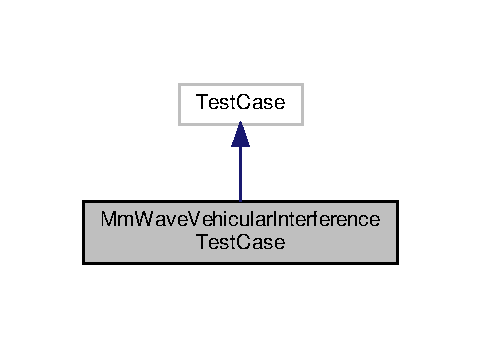
\includegraphics[width=231pt]{classMmWaveVehicularInterferenceTestCase__inherit__graph}
\end{center}
\end{figure}


Collaboration diagram for Mm\+Wave\+Vehicular\+Interference\+Test\+Case\+:
\nopagebreak
\begin{figure}[H]
\begin{center}
\leavevmode
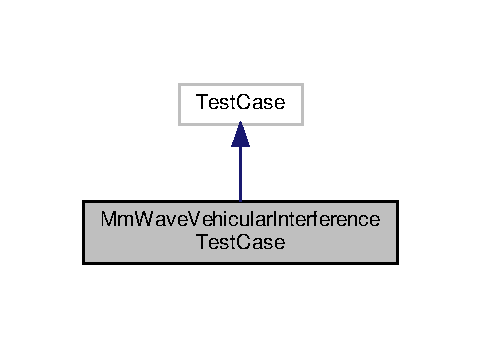
\includegraphics[width=231pt]{classMmWaveVehicularInterferenceTestCase__coll__graph}
\end{center}
\end{figure}
\subsection*{Public Member Functions}
\begin{DoxyCompactItemize}
\item 
\hyperlink{classMmWaveVehicularInterferenceTestCase_af7e416628ec4412169240c22f47cc785}{Mm\+Wave\+Vehicular\+Interference\+Test\+Case} ()
\item 
virtual \hyperlink{classMmWaveVehicularInterferenceTestCase_af0c78db7e4ee5ea2f82747b18c5b46c7}{$\sim$\+Mm\+Wave\+Vehicular\+Interference\+Test\+Case} ()
\item 
\mbox{\Hypertarget{classMmWaveVehicularInterferenceTestCase_a0a52ef59129cd60bee461c7b63df69a7}\label{classMmWaveVehicularInterferenceTestCase_a0a52ef59129cd60bee461c7b63df69a7}} 
void {\bfseries Start\+Test} (double tx\+Power)
\item 
virtual void \hyperlink{classMmWaveVehicularInterferenceTestCase_aa69fae32e19bdd74449c9fb9de554a9f}{Do\+Run} (void)
\end{DoxyCompactItemize}


\subsection{Detailed Description}
The aim of this test is to check whether the interference was evaluated correctly when different groups of nodes are transmitting in the same slot, sharing the same cell. Communication is done using an ideal channel; for this reason, the position of the vehicles does not influence the results. It has been specified just for the sake of giving context to the example. 

\subsection{Constructor \& Destructor Documentation}
\mbox{\Hypertarget{classMmWaveVehicularInterferenceTestCase_af7e416628ec4412169240c22f47cc785}\label{classMmWaveVehicularInterferenceTestCase_af7e416628ec4412169240c22f47cc785}} 
\index{Mm\+Wave\+Vehicular\+Interference\+Test\+Case@{Mm\+Wave\+Vehicular\+Interference\+Test\+Case}!Mm\+Wave\+Vehicular\+Interference\+Test\+Case@{Mm\+Wave\+Vehicular\+Interference\+Test\+Case}}
\index{Mm\+Wave\+Vehicular\+Interference\+Test\+Case@{Mm\+Wave\+Vehicular\+Interference\+Test\+Case}!Mm\+Wave\+Vehicular\+Interference\+Test\+Case@{Mm\+Wave\+Vehicular\+Interference\+Test\+Case}}
\subsubsection{\texorpdfstring{Mm\+Wave\+Vehicular\+Interference\+Test\+Case()}{MmWaveVehicularInterferenceTestCase()}}
{\footnotesize\ttfamily Mm\+Wave\+Vehicular\+Interference\+Test\+Case\+::\+Mm\+Wave\+Vehicular\+Interference\+Test\+Case (\begin{DoxyParamCaption}{ }\end{DoxyParamCaption})}

Constructor \mbox{\Hypertarget{classMmWaveVehicularInterferenceTestCase_af0c78db7e4ee5ea2f82747b18c5b46c7}\label{classMmWaveVehicularInterferenceTestCase_af0c78db7e4ee5ea2f82747b18c5b46c7}} 
\index{Mm\+Wave\+Vehicular\+Interference\+Test\+Case@{Mm\+Wave\+Vehicular\+Interference\+Test\+Case}!````~Mm\+Wave\+Vehicular\+Interference\+Test\+Case@{$\sim$\+Mm\+Wave\+Vehicular\+Interference\+Test\+Case}}
\index{````~Mm\+Wave\+Vehicular\+Interference\+Test\+Case@{$\sim$\+Mm\+Wave\+Vehicular\+Interference\+Test\+Case}!Mm\+Wave\+Vehicular\+Interference\+Test\+Case@{Mm\+Wave\+Vehicular\+Interference\+Test\+Case}}
\subsubsection{\texorpdfstring{$\sim$\+Mm\+Wave\+Vehicular\+Interference\+Test\+Case()}{~MmWaveVehicularInterferenceTestCase()}}
{\footnotesize\ttfamily Mm\+Wave\+Vehicular\+Interference\+Test\+Case\+::$\sim$\+Mm\+Wave\+Vehicular\+Interference\+Test\+Case (\begin{DoxyParamCaption}{ }\end{DoxyParamCaption})\hspace{0.3cm}{\ttfamily [virtual]}}

Destructor 

\subsection{Member Function Documentation}
\mbox{\Hypertarget{classMmWaveVehicularInterferenceTestCase_aa69fae32e19bdd74449c9fb9de554a9f}\label{classMmWaveVehicularInterferenceTestCase_aa69fae32e19bdd74449c9fb9de554a9f}} 
\index{Mm\+Wave\+Vehicular\+Interference\+Test\+Case@{Mm\+Wave\+Vehicular\+Interference\+Test\+Case}!Do\+Run@{Do\+Run}}
\index{Do\+Run@{Do\+Run}!Mm\+Wave\+Vehicular\+Interference\+Test\+Case@{Mm\+Wave\+Vehicular\+Interference\+Test\+Case}}
\subsubsection{\texorpdfstring{Do\+Run()}{DoRun()}}
{\footnotesize\ttfamily void Mm\+Wave\+Vehicular\+Interference\+Test\+Case\+::\+Do\+Run (\begin{DoxyParamCaption}\item[{void}]{ }\end{DoxyParamCaption})\hspace{0.3cm}{\ttfamily [virtual]}}

This method run the test 

The documentation for this class was generated from the following file\+:\begin{DoxyCompactItemize}
\item 
test/mmwave-\/vehicular-\/interference-\/test.\+cc\end{DoxyCompactItemize}

\hypertarget{classMmWaveVehicularInterferenceTestSuite}{}\section{Mm\+Wave\+Vehicular\+Interference\+Test\+Suite Class Reference}
\label{classMmWaveVehicularInterferenceTestSuite}\index{Mm\+Wave\+Vehicular\+Interference\+Test\+Suite@{Mm\+Wave\+Vehicular\+Interference\+Test\+Suite}}


Inheritance diagram for Mm\+Wave\+Vehicular\+Interference\+Test\+Suite\+:\nopagebreak
\begin{figure}[H]
\begin{center}
\leavevmode
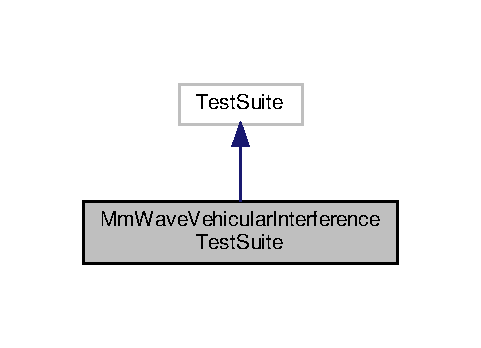
\includegraphics[width=231pt]{classMmWaveVehicularInterferenceTestSuite__inherit__graph}
\end{center}
\end{figure}


Collaboration diagram for Mm\+Wave\+Vehicular\+Interference\+Test\+Suite\+:\nopagebreak
\begin{figure}[H]
\begin{center}
\leavevmode
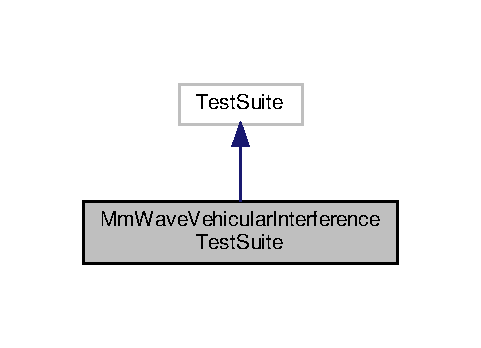
\includegraphics[width=231pt]{classMmWaveVehicularInterferenceTestSuite__coll__graph}
\end{center}
\end{figure}


The documentation for this class was generated from the following file\+:\begin{DoxyCompactItemize}
\item 
test/mmwave-\/vehicular-\/interference-\/test.\+cc\end{DoxyCompactItemize}

\hypertarget{classns3_1_1millicar_1_1MmWaveVehicularNetDevice}{}\section{ns3\+:\+:millicar\+:\+:Mm\+Wave\+Vehicular\+Net\+Device Class Reference}
\label{classns3_1_1millicar_1_1MmWaveVehicularNetDevice}\index{ns3\+::millicar\+::\+Mm\+Wave\+Vehicular\+Net\+Device@{ns3\+::millicar\+::\+Mm\+Wave\+Vehicular\+Net\+Device}}


Inheritance diagram for ns3\+:\+:millicar\+:\+:Mm\+Wave\+Vehicular\+Net\+Device\+:\nopagebreak
\begin{figure}[H]
\begin{center}
\leavevmode
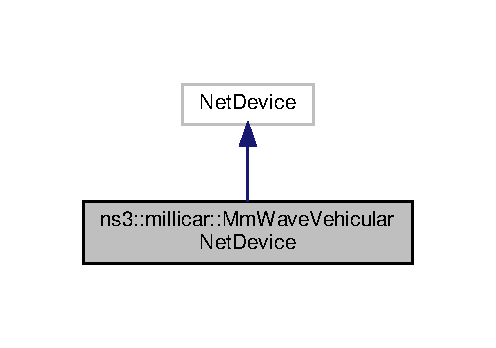
\includegraphics[width=238pt]{classns3_1_1millicar_1_1MmWaveVehicularNetDevice__inherit__graph}
\end{center}
\end{figure}


Collaboration diagram for ns3\+:\+:millicar\+:\+:Mm\+Wave\+Vehicular\+Net\+Device\+:\nopagebreak
\begin{figure}[H]
\begin{center}
\leavevmode
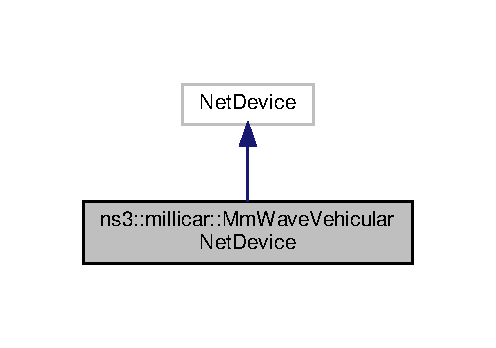
\includegraphics[width=238pt]{classns3_1_1millicar_1_1MmWaveVehicularNetDevice__coll__graph}
\end{center}
\end{figure}
\subsection*{Public Member Functions}
\begin{DoxyCompactItemize}
\item 
\mbox{\Hypertarget{classns3_1_1millicar_1_1MmWaveVehicularNetDevice_abb8b5c9f12799567e525f0bbf44df43f}\label{classns3_1_1millicar_1_1MmWaveVehicularNetDevice_abb8b5c9f12799567e525f0bbf44df43f}} 
\hyperlink{classns3_1_1millicar_1_1MmWaveVehicularNetDevice_abb8b5c9f12799567e525f0bbf44df43f}{Mm\+Wave\+Vehicular\+Net\+Device} (void)
\begin{DoxyCompactList}\small\item\em Class constructor, it is not used. \end{DoxyCompactList}\item 
\hyperlink{classns3_1_1millicar_1_1MmWaveVehicularNetDevice_a45198022453e183d1d0337cd6871d24d}{Mm\+Wave\+Vehicular\+Net\+Device} (Ptr$<$ \hyperlink{classns3_1_1millicar_1_1MmWaveSidelinkPhy}{Mm\+Wave\+Sidelink\+Phy} $>$ phy, Ptr$<$ \hyperlink{classns3_1_1millicar_1_1MmWaveSidelinkMac}{Mm\+Wave\+Sidelink\+Mac} $>$ mac)
\begin{DoxyCompactList}\small\item\em Class constructor. \end{DoxyCompactList}\item 
\mbox{\Hypertarget{classns3_1_1millicar_1_1MmWaveVehicularNetDevice_a31c5848049ce3b89cb9635bb8763b57e}\label{classns3_1_1millicar_1_1MmWaveVehicularNetDevice_a31c5848049ce3b89cb9635bb8763b57e}} 
virtual \hyperlink{classns3_1_1millicar_1_1MmWaveVehicularNetDevice_a31c5848049ce3b89cb9635bb8763b57e}{$\sim$\+Mm\+Wave\+Vehicular\+Net\+Device} (void)
\begin{DoxyCompactList}\small\item\em Class destructor. \end{DoxyCompactList}\item 
\mbox{\Hypertarget{classns3_1_1millicar_1_1MmWaveVehicularNetDevice_a83508411865ea28c89701ccedc00db57}\label{classns3_1_1millicar_1_1MmWaveVehicularNetDevice_a83508411865ea28c89701ccedc00db57}} 
virtual void \hyperlink{classns3_1_1millicar_1_1MmWaveVehicularNetDevice_a83508411865ea28c89701ccedc00db57}{Do\+Dispose} (void)
\begin{DoxyCompactList}\small\item\em Destructor implementation. \end{DoxyCompactList}\item 
\mbox{\Hypertarget{classns3_1_1millicar_1_1MmWaveVehicularNetDevice_a97c6a6dc01d81b119c6d580ca62fe840}\label{classns3_1_1millicar_1_1MmWaveVehicularNetDevice_a97c6a6dc01d81b119c6d580ca62fe840}} 
virtual void {\bfseries Set\+If\+Index} (const uint32\+\_\+t index)
\item 
\mbox{\Hypertarget{classns3_1_1millicar_1_1MmWaveVehicularNetDevice_a660f49a3526c4d45e08e78af663ae62f}\label{classns3_1_1millicar_1_1MmWaveVehicularNetDevice_a660f49a3526c4d45e08e78af663ae62f}} 
virtual uint32\+\_\+t {\bfseries Get\+If\+Index} (void) const
\item 
\mbox{\Hypertarget{classns3_1_1millicar_1_1MmWaveVehicularNetDevice_a268b9fa08b8f726e2e9a1a2f58ead1b1}\label{classns3_1_1millicar_1_1MmWaveVehicularNetDevice_a268b9fa08b8f726e2e9a1a2f58ead1b1}} 
virtual Ptr$<$ Channel $>$ {\bfseries Get\+Channel} (void) const
\item 
\mbox{\Hypertarget{classns3_1_1millicar_1_1MmWaveVehicularNetDevice_a39f42943aa50a1b3e568ae386a6ad586}\label{classns3_1_1millicar_1_1MmWaveVehicularNetDevice_a39f42943aa50a1b3e568ae386a6ad586}} 
virtual bool {\bfseries Is\+Link\+Up} (void) const
\item 
\mbox{\Hypertarget{classns3_1_1millicar_1_1MmWaveVehicularNetDevice_a43363b56aaaec26443913bb6783a3225}\label{classns3_1_1millicar_1_1MmWaveVehicularNetDevice_a43363b56aaaec26443913bb6783a3225}} 
virtual void {\bfseries Add\+Link\+Change\+Callback} (Callback$<$ void $>$ callback)
\item 
\mbox{\Hypertarget{classns3_1_1millicar_1_1MmWaveVehicularNetDevice_a67c7e942d6ae62b1eb8ba44f916220f3}\label{classns3_1_1millicar_1_1MmWaveVehicularNetDevice_a67c7e942d6ae62b1eb8ba44f916220f3}} 
virtual bool {\bfseries Is\+Broadcast} (void) const
\item 
\mbox{\Hypertarget{classns3_1_1millicar_1_1MmWaveVehicularNetDevice_ad685bceec938971ae194bdf6eb343e41}\label{classns3_1_1millicar_1_1MmWaveVehicularNetDevice_ad685bceec938971ae194bdf6eb343e41}} 
virtual Address {\bfseries Get\+Broadcast} (void) const
\item 
\mbox{\Hypertarget{classns3_1_1millicar_1_1MmWaveVehicularNetDevice_a722d78305ef516a719f4e2fde12ed94f}\label{classns3_1_1millicar_1_1MmWaveVehicularNetDevice_a722d78305ef516a719f4e2fde12ed94f}} 
virtual bool {\bfseries Is\+Multicast} (void) const
\item 
\mbox{\Hypertarget{classns3_1_1millicar_1_1MmWaveVehicularNetDevice_a16b8b7724a1d0ae9a9c5114905a27932}\label{classns3_1_1millicar_1_1MmWaveVehicularNetDevice_a16b8b7724a1d0ae9a9c5114905a27932}} 
virtual Address {\bfseries Get\+Multicast} (Ipv4\+Address multicast\+Group) const
\item 
\mbox{\Hypertarget{classns3_1_1millicar_1_1MmWaveVehicularNetDevice_ab8498b22d452c090bbb99bd3557e6126}\label{classns3_1_1millicar_1_1MmWaveVehicularNetDevice_ab8498b22d452c090bbb99bd3557e6126}} 
virtual bool {\bfseries Is\+Bridge} (void) const
\item 
\mbox{\Hypertarget{classns3_1_1millicar_1_1MmWaveVehicularNetDevice_a708cb3cf1d9b318d557b3ed6144918be}\label{classns3_1_1millicar_1_1MmWaveVehicularNetDevice_a708cb3cf1d9b318d557b3ed6144918be}} 
virtual bool {\bfseries Is\+Point\+To\+Point} (void) const
\item 
\mbox{\Hypertarget{classns3_1_1millicar_1_1MmWaveVehicularNetDevice_a37913da22f0cca7f04ef00f05b1176f6}\label{classns3_1_1millicar_1_1MmWaveVehicularNetDevice_a37913da22f0cca7f04ef00f05b1176f6}} 
virtual bool {\bfseries Send\+From} (Ptr$<$ Packet $>$ packet, const Address \&source, const Address \&dest, uint16\+\_\+t protocol\+Number)
\item 
\mbox{\Hypertarget{classns3_1_1millicar_1_1MmWaveVehicularNetDevice_ad1cfc087b6f3972e1b64e016a042569a}\label{classns3_1_1millicar_1_1MmWaveVehicularNetDevice_ad1cfc087b6f3972e1b64e016a042569a}} 
virtual Ptr$<$ Node $>$ {\bfseries Get\+Node} (void) const
\item 
\mbox{\Hypertarget{classns3_1_1millicar_1_1MmWaveVehicularNetDevice_ac07e54a1cc01bf607d3fbe29aec802f0}\label{classns3_1_1millicar_1_1MmWaveVehicularNetDevice_ac07e54a1cc01bf607d3fbe29aec802f0}} 
virtual void {\bfseries Set\+Node} (Ptr$<$ Node $>$ node)
\item 
\mbox{\Hypertarget{classns3_1_1millicar_1_1MmWaveVehicularNetDevice_abe9fb68d56e55a7a9de77989d4671839}\label{classns3_1_1millicar_1_1MmWaveVehicularNetDevice_abe9fb68d56e55a7a9de77989d4671839}} 
virtual bool {\bfseries Needs\+Arp} (void) const
\item 
\mbox{\Hypertarget{classns3_1_1millicar_1_1MmWaveVehicularNetDevice_a30ab5096e57d6d42b000abd4733b57ff}\label{classns3_1_1millicar_1_1MmWaveVehicularNetDevice_a30ab5096e57d6d42b000abd4733b57ff}} 
virtual Address {\bfseries Get\+Multicast} (Ipv6\+Address addr) const
\item 
\mbox{\Hypertarget{classns3_1_1millicar_1_1MmWaveVehicularNetDevice_a5207726b256796df9dbb4aae6615d21f}\label{classns3_1_1millicar_1_1MmWaveVehicularNetDevice_a5207726b256796df9dbb4aae6615d21f}} 
virtual void {\bfseries Set\+Receive\+Callback} (Receive\+Callback cb)
\item 
\mbox{\Hypertarget{classns3_1_1millicar_1_1MmWaveVehicularNetDevice_a1f508820c02dce66bcb71fdf4a006909}\label{classns3_1_1millicar_1_1MmWaveVehicularNetDevice_a1f508820c02dce66bcb71fdf4a006909}} 
virtual void {\bfseries Set\+Promisc\+Receive\+Callback} (Promisc\+Receive\+Callback cb)
\item 
\mbox{\Hypertarget{classns3_1_1millicar_1_1MmWaveVehicularNetDevice_a69dd9d59a5d72b632e7b42e55daa5835}\label{classns3_1_1millicar_1_1MmWaveVehicularNetDevice_a69dd9d59a5d72b632e7b42e55daa5835}} 
virtual bool {\bfseries Supports\+Send\+From} (void) const
\item 
virtual void \hyperlink{classns3_1_1millicar_1_1MmWaveVehicularNetDevice_a3932dafc57cc997401c3d0d14d647287}{Set\+Address} (Address address)
\begin{DoxyCompactList}\small\item\em Set M\+AC address associated to the Net\+Device. \end{DoxyCompactList}\item 
\mbox{\Hypertarget{classns3_1_1millicar_1_1MmWaveVehicularNetDevice_a387893f7a3fe0eb9db5505d0ade5c583}\label{classns3_1_1millicar_1_1MmWaveVehicularNetDevice_a387893f7a3fe0eb9db5505d0ade5c583}} 
virtual Address \hyperlink{classns3_1_1millicar_1_1MmWaveVehicularNetDevice_a387893f7a3fe0eb9db5505d0ade5c583}{Get\+Address} (void) const
\begin{DoxyCompactList}\small\item\em Returns M\+AC address associated to the Net\+Device. \end{DoxyCompactList}\item 
\mbox{\Hypertarget{classns3_1_1millicar_1_1MmWaveVehicularNetDevice_a840697a126197bbbc7d71ac4250fb39c}\label{classns3_1_1millicar_1_1MmWaveVehicularNetDevice_a840697a126197bbbc7d71ac4250fb39c}} 
virtual Ptr$<$ \hyperlink{classns3_1_1millicar_1_1MmWaveSidelinkMac}{Mm\+Wave\+Sidelink\+Mac} $>$ \hyperlink{classns3_1_1millicar_1_1MmWaveVehicularNetDevice_a840697a126197bbbc7d71ac4250fb39c}{Get\+Mac} (void) const
\begin{DoxyCompactList}\small\item\em Returns pointer to M\+AC. \end{DoxyCompactList}\item 
\mbox{\Hypertarget{classns3_1_1millicar_1_1MmWaveVehicularNetDevice_aec2c2afec33925b2186204d2bae3d080}\label{classns3_1_1millicar_1_1MmWaveVehicularNetDevice_aec2c2afec33925b2186204d2bae3d080}} 
virtual Ptr$<$ \hyperlink{classns3_1_1millicar_1_1MmWaveSidelinkPhy}{Mm\+Wave\+Sidelink\+Phy} $>$ \hyperlink{classns3_1_1millicar_1_1MmWaveVehicularNetDevice_aec2c2afec33925b2186204d2bae3d080}{Get\+Phy} (void) const
\begin{DoxyCompactList}\small\item\em Returns pointer to P\+HY. \end{DoxyCompactList}\item 
virtual bool \hyperlink{classns3_1_1millicar_1_1MmWaveVehicularNetDevice_a60c5982f9d3aeab8de2dfdfaec142a2f}{Send} (Ptr$<$ Packet $>$ packet, const Address \&dest, uint16\+\_\+t protocol\+Number)
\begin{DoxyCompactList}\small\item\em Send a packet to the vehicular stack. \end{DoxyCompactList}\item 
virtual bool \hyperlink{classns3_1_1millicar_1_1MmWaveVehicularNetDevice_a5e381e54c479300f0f4180227d810bae}{Set\+Mtu} (const uint16\+\_\+t mtu)
\begin{DoxyCompactList}\small\item\em Set M\+TU associated to the Net\+Device. \end{DoxyCompactList}\item 
\mbox{\Hypertarget{classns3_1_1millicar_1_1MmWaveVehicularNetDevice_a706437862864c4c34c6b2beb88b3b307}\label{classns3_1_1millicar_1_1MmWaveVehicularNetDevice_a706437862864c4c34c6b2beb88b3b307}} 
virtual uint16\+\_\+t \hyperlink{classns3_1_1millicar_1_1MmWaveVehicularNetDevice_a706437862864c4c34c6b2beb88b3b307}{Get\+Mtu} (void) const
\begin{DoxyCompactList}\small\item\em Returns M\+TU associated to the Net\+Device. \end{DoxyCompactList}\item 
Type\+Id \hyperlink{classns3_1_1millicar_1_1MmWaveVehicularNetDevice_a203a3fd59d76d45088f1921aff413549}{Get\+Rlc\+Type} (std\+::string rlc\+Type)
\begin{DoxyCompactList}\small\item\em Returns valid Lte\+Rlc Type\+Id based on the parameter passed. \end{DoxyCompactList}\item 
void \hyperlink{classns3_1_1millicar_1_1MmWaveVehicularNetDevice_a039f27547bec8a9eeea418b47241a578}{Receive} (Ptr$<$ Packet $>$ p)
\begin{DoxyCompactList}\small\item\em Packet forwarding to the M\+AC layer by calling Do\+Transmit\+Pdu. \end{DoxyCompactList}\item 
void \hyperlink{classns3_1_1millicar_1_1MmWaveVehicularNetDevice_a9a94cdd2a634545069bc76a25e48d5e7}{Activate\+Bearer} (const uint8\+\_\+t bearer\+Id, const uint16\+\_\+t dest\+Rnti, const Address \&dest)
\begin{DoxyCompactList}\small\item\em a logical channel with instances of P\+D\+C\+P/\+R\+LC layers is created and associated to a specific receiving device \end{DoxyCompactList}\end{DoxyCompactItemize}
\subsection*{Static Public Member Functions}
\begin{DoxyCompactItemize}
\item 
static Type\+Id \hyperlink{classns3_1_1millicar_1_1MmWaveVehicularNetDevice_a5d96b39b9b59c2daa4068b6a302358fd}{Get\+Type\+Id} (void)
\begin{DoxyCompactList}\small\item\em Get the type ID. \end{DoxyCompactList}\end{DoxyCompactItemize}
\subsection*{Protected Attributes}
\begin{DoxyCompactItemize}
\item 
\mbox{\Hypertarget{classns3_1_1millicar_1_1MmWaveVehicularNetDevice_a9afc224b7198420bfe70b811809e6337}\label{classns3_1_1millicar_1_1MmWaveVehicularNetDevice_a9afc224b7198420bfe70b811809e6337}} 
Net\+Device\+::\+Receive\+Callback \hyperlink{classns3_1_1millicar_1_1MmWaveVehicularNetDevice_a9afc224b7198420bfe70b811809e6337}{m\+\_\+rx\+Callback}
\begin{DoxyCompactList}\small\item\em callback that is fired when a packet is received \end{DoxyCompactList}\end{DoxyCompactItemize}


\subsection{Constructor \& Destructor Documentation}
\mbox{\Hypertarget{classns3_1_1millicar_1_1MmWaveVehicularNetDevice_a45198022453e183d1d0337cd6871d24d}\label{classns3_1_1millicar_1_1MmWaveVehicularNetDevice_a45198022453e183d1d0337cd6871d24d}} 
\index{ns3\+::millicar\+::\+Mm\+Wave\+Vehicular\+Net\+Device@{ns3\+::millicar\+::\+Mm\+Wave\+Vehicular\+Net\+Device}!Mm\+Wave\+Vehicular\+Net\+Device@{Mm\+Wave\+Vehicular\+Net\+Device}}
\index{Mm\+Wave\+Vehicular\+Net\+Device@{Mm\+Wave\+Vehicular\+Net\+Device}!ns3\+::millicar\+::\+Mm\+Wave\+Vehicular\+Net\+Device@{ns3\+::millicar\+::\+Mm\+Wave\+Vehicular\+Net\+Device}}
\subsubsection{\texorpdfstring{Mm\+Wave\+Vehicular\+Net\+Device()}{MmWaveVehicularNetDevice()}}
{\footnotesize\ttfamily ns3\+::millicar\+::\+Mm\+Wave\+Vehicular\+Net\+Device\+::\+Mm\+Wave\+Vehicular\+Net\+Device (\begin{DoxyParamCaption}\item[{Ptr$<$ \hyperlink{classns3_1_1millicar_1_1MmWaveSidelinkPhy}{Mm\+Wave\+Sidelink\+Phy} $>$}]{phy,  }\item[{Ptr$<$ \hyperlink{classns3_1_1millicar_1_1MmWaveSidelinkMac}{Mm\+Wave\+Sidelink\+Mac} $>$}]{mac }\end{DoxyParamCaption})}



Class constructor. 


\begin{DoxyParams}{Parameters}
{\em phy} & pointer to the P\+HY \\
\hline
{\em mac} & pointer to the M\+AC \\
\hline
\end{DoxyParams}


\subsection{Member Function Documentation}
\mbox{\Hypertarget{classns3_1_1millicar_1_1MmWaveVehicularNetDevice_a9a94cdd2a634545069bc76a25e48d5e7}\label{classns3_1_1millicar_1_1MmWaveVehicularNetDevice_a9a94cdd2a634545069bc76a25e48d5e7}} 
\index{ns3\+::millicar\+::\+Mm\+Wave\+Vehicular\+Net\+Device@{ns3\+::millicar\+::\+Mm\+Wave\+Vehicular\+Net\+Device}!Activate\+Bearer@{Activate\+Bearer}}
\index{Activate\+Bearer@{Activate\+Bearer}!ns3\+::millicar\+::\+Mm\+Wave\+Vehicular\+Net\+Device@{ns3\+::millicar\+::\+Mm\+Wave\+Vehicular\+Net\+Device}}
\subsubsection{\texorpdfstring{Activate\+Bearer()}{ActivateBearer()}}
{\footnotesize\ttfamily void ns3\+::millicar\+::\+Mm\+Wave\+Vehicular\+Net\+Device\+::\+Activate\+Bearer (\begin{DoxyParamCaption}\item[{const uint8\+\_\+t}]{bearer\+Id,  }\item[{const uint16\+\_\+t}]{dest\+Rnti,  }\item[{const Address \&}]{dest }\end{DoxyParamCaption})}



a logical channel with instances of P\+D\+C\+P/\+R\+LC layers is created and associated to a specific receiving device 


\begin{DoxyParams}{Parameters}
{\em bearer\+Id} & identifier of the tunnel between two devices \\
\hline
{\em dest\+Rnti} & the rnti of the destination \\
\hline
{\em dest} & IP destination address \\
\hline
\end{DoxyParams}
\mbox{\Hypertarget{classns3_1_1millicar_1_1MmWaveVehicularNetDevice_a203a3fd59d76d45088f1921aff413549}\label{classns3_1_1millicar_1_1MmWaveVehicularNetDevice_a203a3fd59d76d45088f1921aff413549}} 
\index{ns3\+::millicar\+::\+Mm\+Wave\+Vehicular\+Net\+Device@{ns3\+::millicar\+::\+Mm\+Wave\+Vehicular\+Net\+Device}!Get\+Rlc\+Type@{Get\+Rlc\+Type}}
\index{Get\+Rlc\+Type@{Get\+Rlc\+Type}!ns3\+::millicar\+::\+Mm\+Wave\+Vehicular\+Net\+Device@{ns3\+::millicar\+::\+Mm\+Wave\+Vehicular\+Net\+Device}}
\subsubsection{\texorpdfstring{Get\+Rlc\+Type()}{GetRlcType()}}
{\footnotesize\ttfamily Type\+Id ns3\+::millicar\+::\+Mm\+Wave\+Vehicular\+Net\+Device\+::\+Get\+Rlc\+Type (\begin{DoxyParamCaption}\item[{std\+::string}]{rlc\+Type }\end{DoxyParamCaption})}



Returns valid Lte\+Rlc Type\+Id based on the parameter passed. 


\begin{DoxyParams}{Parameters}
{\em rlc\+Type} & string representing the selected R\+LC type \\
\hline
\end{DoxyParams}
\begin{DoxyReturn}{Returns}
the type id of the proper R\+LC class 
\end{DoxyReturn}
\mbox{\Hypertarget{classns3_1_1millicar_1_1MmWaveVehicularNetDevice_a5d96b39b9b59c2daa4068b6a302358fd}\label{classns3_1_1millicar_1_1MmWaveVehicularNetDevice_a5d96b39b9b59c2daa4068b6a302358fd}} 
\index{ns3\+::millicar\+::\+Mm\+Wave\+Vehicular\+Net\+Device@{ns3\+::millicar\+::\+Mm\+Wave\+Vehicular\+Net\+Device}!Get\+Type\+Id@{Get\+Type\+Id}}
\index{Get\+Type\+Id@{Get\+Type\+Id}!ns3\+::millicar\+::\+Mm\+Wave\+Vehicular\+Net\+Device@{ns3\+::millicar\+::\+Mm\+Wave\+Vehicular\+Net\+Device}}
\subsubsection{\texorpdfstring{Get\+Type\+Id()}{GetTypeId()}}
{\footnotesize\ttfamily Type\+Id ns3\+::millicar\+::\+Mm\+Wave\+Vehicular\+Net\+Device\+::\+Get\+Type\+Id (\begin{DoxyParamCaption}\item[{void}]{ }\end{DoxyParamCaption})\hspace{0.3cm}{\ttfamily [static]}}



Get the type ID. 

\begin{DoxyReturn}{Returns}
the object Type\+Id 
\end{DoxyReturn}
\mbox{\Hypertarget{classns3_1_1millicar_1_1MmWaveVehicularNetDevice_a039f27547bec8a9eeea418b47241a578}\label{classns3_1_1millicar_1_1MmWaveVehicularNetDevice_a039f27547bec8a9eeea418b47241a578}} 
\index{ns3\+::millicar\+::\+Mm\+Wave\+Vehicular\+Net\+Device@{ns3\+::millicar\+::\+Mm\+Wave\+Vehicular\+Net\+Device}!Receive@{Receive}}
\index{Receive@{Receive}!ns3\+::millicar\+::\+Mm\+Wave\+Vehicular\+Net\+Device@{ns3\+::millicar\+::\+Mm\+Wave\+Vehicular\+Net\+Device}}
\subsubsection{\texorpdfstring{Receive()}{Receive()}}
{\footnotesize\ttfamily void ns3\+::millicar\+::\+Mm\+Wave\+Vehicular\+Net\+Device\+::\+Receive (\begin{DoxyParamCaption}\item[{Ptr$<$ Packet $>$}]{p }\end{DoxyParamCaption})}



Packet forwarding to the M\+AC layer by calling Do\+Transmit\+Pdu. 


\begin{DoxyParams}{Parameters}
{\em p} & packet to be used to fire the callbacks \\
\hline
\end{DoxyParams}
\mbox{\Hypertarget{classns3_1_1millicar_1_1MmWaveVehicularNetDevice_a60c5982f9d3aeab8de2dfdfaec142a2f}\label{classns3_1_1millicar_1_1MmWaveVehicularNetDevice_a60c5982f9d3aeab8de2dfdfaec142a2f}} 
\index{ns3\+::millicar\+::\+Mm\+Wave\+Vehicular\+Net\+Device@{ns3\+::millicar\+::\+Mm\+Wave\+Vehicular\+Net\+Device}!Send@{Send}}
\index{Send@{Send}!ns3\+::millicar\+::\+Mm\+Wave\+Vehicular\+Net\+Device@{ns3\+::millicar\+::\+Mm\+Wave\+Vehicular\+Net\+Device}}
\subsubsection{\texorpdfstring{Send()}{Send()}}
{\footnotesize\ttfamily bool ns3\+::millicar\+::\+Mm\+Wave\+Vehicular\+Net\+Device\+::\+Send (\begin{DoxyParamCaption}\item[{Ptr$<$ Packet $>$}]{packet,  }\item[{const Address \&}]{dest,  }\item[{uint16\+\_\+t}]{protocol\+Number }\end{DoxyParamCaption})\hspace{0.3cm}{\ttfamily [virtual]}}



Send a packet to the vehicular stack. 


\begin{DoxyParams}{Parameters}
{\em address} & M\+AC address of the destination device \\
\hline
{\em protocol\+Number} & identifies if Net\+Device is using I\+Pv4 or I\+Pv6 \\
\hline
\end{DoxyParams}
\mbox{\Hypertarget{classns3_1_1millicar_1_1MmWaveVehicularNetDevice_a3932dafc57cc997401c3d0d14d647287}\label{classns3_1_1millicar_1_1MmWaveVehicularNetDevice_a3932dafc57cc997401c3d0d14d647287}} 
\index{ns3\+::millicar\+::\+Mm\+Wave\+Vehicular\+Net\+Device@{ns3\+::millicar\+::\+Mm\+Wave\+Vehicular\+Net\+Device}!Set\+Address@{Set\+Address}}
\index{Set\+Address@{Set\+Address}!ns3\+::millicar\+::\+Mm\+Wave\+Vehicular\+Net\+Device@{ns3\+::millicar\+::\+Mm\+Wave\+Vehicular\+Net\+Device}}
\subsubsection{\texorpdfstring{Set\+Address()}{SetAddress()}}
{\footnotesize\ttfamily void ns3\+::millicar\+::\+Mm\+Wave\+Vehicular\+Net\+Device\+::\+Set\+Address (\begin{DoxyParamCaption}\item[{Address}]{address }\end{DoxyParamCaption})\hspace{0.3cm}{\ttfamily [virtual]}}



Set M\+AC address associated to the Net\+Device. 


\begin{DoxyParams}{Parameters}
{\em address} & M\+AC address \\
\hline
\end{DoxyParams}
\mbox{\Hypertarget{classns3_1_1millicar_1_1MmWaveVehicularNetDevice_a5e381e54c479300f0f4180227d810bae}\label{classns3_1_1millicar_1_1MmWaveVehicularNetDevice_a5e381e54c479300f0f4180227d810bae}} 
\index{ns3\+::millicar\+::\+Mm\+Wave\+Vehicular\+Net\+Device@{ns3\+::millicar\+::\+Mm\+Wave\+Vehicular\+Net\+Device}!Set\+Mtu@{Set\+Mtu}}
\index{Set\+Mtu@{Set\+Mtu}!ns3\+::millicar\+::\+Mm\+Wave\+Vehicular\+Net\+Device@{ns3\+::millicar\+::\+Mm\+Wave\+Vehicular\+Net\+Device}}
\subsubsection{\texorpdfstring{Set\+Mtu()}{SetMtu()}}
{\footnotesize\ttfamily bool ns3\+::millicar\+::\+Mm\+Wave\+Vehicular\+Net\+Device\+::\+Set\+Mtu (\begin{DoxyParamCaption}\item[{const uint16\+\_\+t}]{mtu }\end{DoxyParamCaption})\hspace{0.3cm}{\ttfamily [virtual]}}



Set M\+TU associated to the Net\+Device. 


\begin{DoxyParams}{Parameters}
{\em mtu} & size of the Maximum Transmission Unit \\
\hline
\end{DoxyParams}


The documentation for this class was generated from the following files\+:\begin{DoxyCompactItemize}
\item 
model/mmwave-\/vehicular-\/net-\/device.\+h\item 
model/mmwave-\/vehicular-\/net-\/device.\+cc\end{DoxyCompactItemize}

\hypertarget{classns3_1_1millicar_1_1MmWaveVehicularPropagationLossModel}{}\section{ns3\+:\+:millicar\+:\+:Mm\+Wave\+Vehicular\+Propagation\+Loss\+Model Class Reference}
\label{classns3_1_1millicar_1_1MmWaveVehicularPropagationLossModel}\index{ns3\+::millicar\+::\+Mm\+Wave\+Vehicular\+Propagation\+Loss\+Model@{ns3\+::millicar\+::\+Mm\+Wave\+Vehicular\+Propagation\+Loss\+Model}}


Inheritance diagram for ns3\+:\+:millicar\+:\+:Mm\+Wave\+Vehicular\+Propagation\+Loss\+Model\+:\nopagebreak
\begin{figure}[H]
\begin{center}
\leavevmode
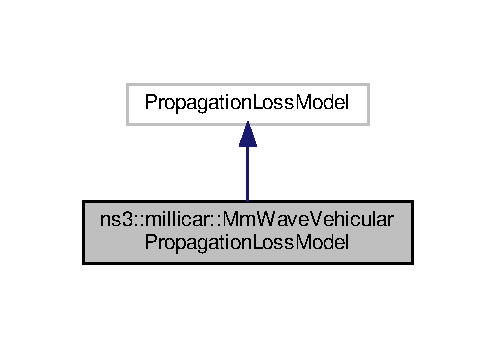
\includegraphics[width=238pt]{classns3_1_1millicar_1_1MmWaveVehicularPropagationLossModel__inherit__graph}
\end{center}
\end{figure}


Collaboration diagram for ns3\+:\+:millicar\+:\+:Mm\+Wave\+Vehicular\+Propagation\+Loss\+Model\+:\nopagebreak
\begin{figure}[H]
\begin{center}
\leavevmode
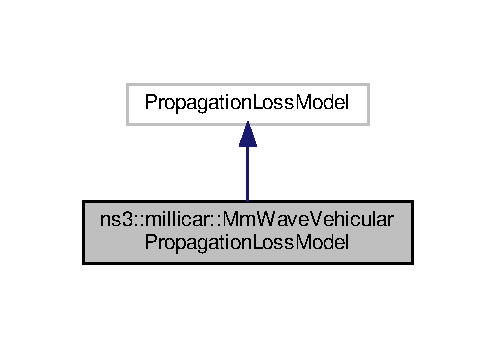
\includegraphics[width=238pt]{classns3_1_1millicar_1_1MmWaveVehicularPropagationLossModel__coll__graph}
\end{center}
\end{figure}
\subsection*{Public Member Functions}
\begin{DoxyCompactItemize}
\item 
void \hyperlink{classns3_1_1millicar_1_1MmWaveVehicularPropagationLossModel_a25532b53a7b9552b09af5a083a17034f}{Set\+Min\+Loss} (double min\+Loss)
\item 
double \hyperlink{classns3_1_1millicar_1_1MmWaveVehicularPropagationLossModel_a1f9733beb4afa3cea41bb64d105c6d75}{Get\+Min\+Loss} (void) const
\item 
void \hyperlink{classns3_1_1millicar_1_1MmWaveVehicularPropagationLossModel_a893c89bb8594342511ef88e4acca3dfe}{Set\+Frequency} (double freq)
\item 
double \hyperlink{classns3_1_1millicar_1_1MmWaveVehicularPropagationLossModel_a4f36d3834b45b62a214acb976e2ae41a}{Get\+Frequency} (void) const
\item 
\mbox{\Hypertarget{classns3_1_1millicar_1_1MmWaveVehicularPropagationLossModel_a980a03d5e0fc5885bbcdd235d4b88e9d}\label{classns3_1_1millicar_1_1MmWaveVehicularPropagationLossModel_a980a03d5e0fc5885bbcdd235d4b88e9d}} 
char {\bfseries Get\+Channel\+Condition} (Ptr$<$ Mobility\+Model $>$ a, Ptr$<$ Mobility\+Model $>$ b)
\item 
\mbox{\Hypertarget{classns3_1_1millicar_1_1MmWaveVehicularPropagationLossModel_acea3ba3d88275e90fbca748948956467}\label{classns3_1_1millicar_1_1MmWaveVehicularPropagationLossModel_acea3ba3d88275e90fbca748948956467}} 
std\+::string {\bfseries Get\+Scenario} ()
\item 
\mbox{\Hypertarget{classns3_1_1millicar_1_1MmWaveVehicularPropagationLossModel_a4dc5e0633643b299cc2d855f8691ec64}\label{classns3_1_1millicar_1_1MmWaveVehicularPropagationLossModel_a4dc5e0633643b299cc2d855f8691ec64}} 
double {\bfseries Get\+Loss} (Ptr$<$ Mobility\+Model $>$ a, Ptr$<$ Mobility\+Model $>$ b) const
\end{DoxyCompactItemize}
\subsection*{Static Public Member Functions}
\begin{DoxyCompactItemize}
\item 
\mbox{\Hypertarget{classns3_1_1millicar_1_1MmWaveVehicularPropagationLossModel_a1a05885ed5c37249cdf570ced2949a15}\label{classns3_1_1millicar_1_1MmWaveVehicularPropagationLossModel_a1a05885ed5c37249cdf570ced2949a15}} 
static Type\+Id {\bfseries Get\+Type\+Id} (void)
\end{DoxyCompactItemize}


\subsection{Member Function Documentation}
\mbox{\Hypertarget{classns3_1_1millicar_1_1MmWaveVehicularPropagationLossModel_a4f36d3834b45b62a214acb976e2ae41a}\label{classns3_1_1millicar_1_1MmWaveVehicularPropagationLossModel_a4f36d3834b45b62a214acb976e2ae41a}} 
\index{ns3\+::millicar\+::\+Mm\+Wave\+Vehicular\+Propagation\+Loss\+Model@{ns3\+::millicar\+::\+Mm\+Wave\+Vehicular\+Propagation\+Loss\+Model}!Get\+Frequency@{Get\+Frequency}}
\index{Get\+Frequency@{Get\+Frequency}!ns3\+::millicar\+::\+Mm\+Wave\+Vehicular\+Propagation\+Loss\+Model@{ns3\+::millicar\+::\+Mm\+Wave\+Vehicular\+Propagation\+Loss\+Model}}
\subsubsection{\texorpdfstring{Get\+Frequency()}{GetFrequency()}}
{\footnotesize\ttfamily double ns3\+::millicar\+::\+Mm\+Wave\+Vehicular\+Propagation\+Loss\+Model\+::\+Get\+Frequency (\begin{DoxyParamCaption}\item[{void}]{ }\end{DoxyParamCaption}) const}

\begin{DoxyReturn}{Returns}
the current frequency (Hz) 
\end{DoxyReturn}
\mbox{\Hypertarget{classns3_1_1millicar_1_1MmWaveVehicularPropagationLossModel_a1f9733beb4afa3cea41bb64d105c6d75}\label{classns3_1_1millicar_1_1MmWaveVehicularPropagationLossModel_a1f9733beb4afa3cea41bb64d105c6d75}} 
\index{ns3\+::millicar\+::\+Mm\+Wave\+Vehicular\+Propagation\+Loss\+Model@{ns3\+::millicar\+::\+Mm\+Wave\+Vehicular\+Propagation\+Loss\+Model}!Get\+Min\+Loss@{Get\+Min\+Loss}}
\index{Get\+Min\+Loss@{Get\+Min\+Loss}!ns3\+::millicar\+::\+Mm\+Wave\+Vehicular\+Propagation\+Loss\+Model@{ns3\+::millicar\+::\+Mm\+Wave\+Vehicular\+Propagation\+Loss\+Model}}
\subsubsection{\texorpdfstring{Get\+Min\+Loss()}{GetMinLoss()}}
{\footnotesize\ttfamily double ns3\+::millicar\+::\+Mm\+Wave\+Vehicular\+Propagation\+Loss\+Model\+::\+Get\+Min\+Loss (\begin{DoxyParamCaption}\item[{void}]{ }\end{DoxyParamCaption}) const}

\begin{DoxyReturn}{Returns}
the minimum loss. 
\end{DoxyReturn}
\mbox{\Hypertarget{classns3_1_1millicar_1_1MmWaveVehicularPropagationLossModel_a893c89bb8594342511ef88e4acca3dfe}\label{classns3_1_1millicar_1_1MmWaveVehicularPropagationLossModel_a893c89bb8594342511ef88e4acca3dfe}} 
\index{ns3\+::millicar\+::\+Mm\+Wave\+Vehicular\+Propagation\+Loss\+Model@{ns3\+::millicar\+::\+Mm\+Wave\+Vehicular\+Propagation\+Loss\+Model}!Set\+Frequency@{Set\+Frequency}}
\index{Set\+Frequency@{Set\+Frequency}!ns3\+::millicar\+::\+Mm\+Wave\+Vehicular\+Propagation\+Loss\+Model@{ns3\+::millicar\+::\+Mm\+Wave\+Vehicular\+Propagation\+Loss\+Model}}
\subsubsection{\texorpdfstring{Set\+Frequency()}{SetFrequency()}}
{\footnotesize\ttfamily void ns3\+::millicar\+::\+Mm\+Wave\+Vehicular\+Propagation\+Loss\+Model\+::\+Set\+Frequency (\begin{DoxyParamCaption}\item[{double}]{freq }\end{DoxyParamCaption})}


\begin{DoxyParams}{Parameters}
{\em freq} & the operating frequency (Hz) \\
\hline
\end{DoxyParams}
\mbox{\Hypertarget{classns3_1_1millicar_1_1MmWaveVehicularPropagationLossModel_a25532b53a7b9552b09af5a083a17034f}\label{classns3_1_1millicar_1_1MmWaveVehicularPropagationLossModel_a25532b53a7b9552b09af5a083a17034f}} 
\index{ns3\+::millicar\+::\+Mm\+Wave\+Vehicular\+Propagation\+Loss\+Model@{ns3\+::millicar\+::\+Mm\+Wave\+Vehicular\+Propagation\+Loss\+Model}!Set\+Min\+Loss@{Set\+Min\+Loss}}
\index{Set\+Min\+Loss@{Set\+Min\+Loss}!ns3\+::millicar\+::\+Mm\+Wave\+Vehicular\+Propagation\+Loss\+Model@{ns3\+::millicar\+::\+Mm\+Wave\+Vehicular\+Propagation\+Loss\+Model}}
\subsubsection{\texorpdfstring{Set\+Min\+Loss()}{SetMinLoss()}}
{\footnotesize\ttfamily void ns3\+::millicar\+::\+Mm\+Wave\+Vehicular\+Propagation\+Loss\+Model\+::\+Set\+Min\+Loss (\begin{DoxyParamCaption}\item[{double}]{min\+Loss }\end{DoxyParamCaption})}


\begin{DoxyParams}{Parameters}
{\em min\+Loss} & the minimum loss (dB)\\
\hline
\end{DoxyParams}
no matter how short the distance, the total propagation loss (in dB) will always be greater or equal than this value 

The documentation for this class was generated from the following files\+:\begin{DoxyCompactItemize}
\item 
model/mmwave-\/vehicular-\/propagation-\/loss-\/model.\+h\item 
model/mmwave-\/vehicular-\/propagation-\/loss-\/model.\+cc\end{DoxyCompactItemize}

\hypertarget{classMmWaveVehicularRateTestCase}{}\section{Mm\+Wave\+Vehicular\+Rate\+Test\+Case Class Reference}
\label{classMmWaveVehicularRateTestCase}\index{Mm\+Wave\+Vehicular\+Rate\+Test\+Case@{Mm\+Wave\+Vehicular\+Rate\+Test\+Case}}


Inheritance diagram for Mm\+Wave\+Vehicular\+Rate\+Test\+Case\+:\nopagebreak
\begin{figure}[H]
\begin{center}
\leavevmode
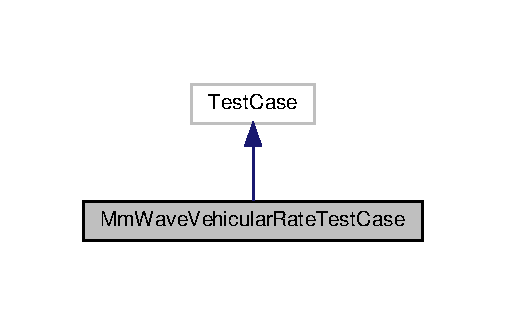
\includegraphics[width=243pt]{classMmWaveVehicularRateTestCase__inherit__graph}
\end{center}
\end{figure}


Collaboration diagram for Mm\+Wave\+Vehicular\+Rate\+Test\+Case\+:\nopagebreak
\begin{figure}[H]
\begin{center}
\leavevmode
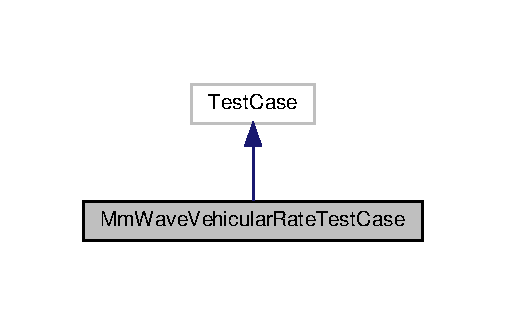
\includegraphics[width=243pt]{classMmWaveVehicularRateTestCase__coll__graph}
\end{center}
\end{figure}
\subsection*{Public Member Functions}
\begin{DoxyCompactItemize}
\item 
\hyperlink{classMmWaveVehicularRateTestCase_a3e2b124bb19443c51bbb945164783fc9}{Mm\+Wave\+Vehicular\+Rate\+Test\+Case} ()
\item 
virtual \hyperlink{classMmWaveVehicularRateTestCase_a83287f6a2eb13810a640a6b0afe4488e}{$\sim$\+Mm\+Wave\+Vehicular\+Rate\+Test\+Case} ()
\item 
\mbox{\Hypertarget{classMmWaveVehicularRateTestCase_a8e2c0002d701bc8f83913b60108d2f45}\label{classMmWaveVehicularRateTestCase_a8e2c0002d701bc8f83913b60108d2f45}} 
void {\bfseries Start\+Test} (uint8\+\_\+t mcs)
\item 
virtual void \hyperlink{classMmWaveVehicularRateTestCase_aa22f2f029bf2ebad00c01d80e9e93e58}{Do\+Run} (void)
\end{DoxyCompactItemize}


\subsection{Detailed Description}
This is a test to check if the designed vehicular stack (M\+AC and P\+HY) is able to run on a basic scenario\+: two vehicle moving at constant velocity and constant distance. The distance increases among different tests of the suite. 

\subsection{Constructor \& Destructor Documentation}
\mbox{\Hypertarget{classMmWaveVehicularRateTestCase_a3e2b124bb19443c51bbb945164783fc9}\label{classMmWaveVehicularRateTestCase_a3e2b124bb19443c51bbb945164783fc9}} 
\index{Mm\+Wave\+Vehicular\+Rate\+Test\+Case@{Mm\+Wave\+Vehicular\+Rate\+Test\+Case}!Mm\+Wave\+Vehicular\+Rate\+Test\+Case@{Mm\+Wave\+Vehicular\+Rate\+Test\+Case}}
\index{Mm\+Wave\+Vehicular\+Rate\+Test\+Case@{Mm\+Wave\+Vehicular\+Rate\+Test\+Case}!Mm\+Wave\+Vehicular\+Rate\+Test\+Case@{Mm\+Wave\+Vehicular\+Rate\+Test\+Case}}
\subsubsection{\texorpdfstring{Mm\+Wave\+Vehicular\+Rate\+Test\+Case()}{MmWaveVehicularRateTestCase()}}
{\footnotesize\ttfamily Mm\+Wave\+Vehicular\+Rate\+Test\+Case\+::\+Mm\+Wave\+Vehicular\+Rate\+Test\+Case (\begin{DoxyParamCaption}{ }\end{DoxyParamCaption})}

Constructor \mbox{\Hypertarget{classMmWaveVehicularRateTestCase_a83287f6a2eb13810a640a6b0afe4488e}\label{classMmWaveVehicularRateTestCase_a83287f6a2eb13810a640a6b0afe4488e}} 
\index{Mm\+Wave\+Vehicular\+Rate\+Test\+Case@{Mm\+Wave\+Vehicular\+Rate\+Test\+Case}!````~Mm\+Wave\+Vehicular\+Rate\+Test\+Case@{$\sim$\+Mm\+Wave\+Vehicular\+Rate\+Test\+Case}}
\index{````~Mm\+Wave\+Vehicular\+Rate\+Test\+Case@{$\sim$\+Mm\+Wave\+Vehicular\+Rate\+Test\+Case}!Mm\+Wave\+Vehicular\+Rate\+Test\+Case@{Mm\+Wave\+Vehicular\+Rate\+Test\+Case}}
\subsubsection{\texorpdfstring{$\sim$\+Mm\+Wave\+Vehicular\+Rate\+Test\+Case()}{~MmWaveVehicularRateTestCase()}}
{\footnotesize\ttfamily Mm\+Wave\+Vehicular\+Rate\+Test\+Case\+::$\sim$\+Mm\+Wave\+Vehicular\+Rate\+Test\+Case (\begin{DoxyParamCaption}{ }\end{DoxyParamCaption})\hspace{0.3cm}{\ttfamily [virtual]}}

Destructor 

\subsection{Member Function Documentation}
\mbox{\Hypertarget{classMmWaveVehicularRateTestCase_aa22f2f029bf2ebad00c01d80e9e93e58}\label{classMmWaveVehicularRateTestCase_aa22f2f029bf2ebad00c01d80e9e93e58}} 
\index{Mm\+Wave\+Vehicular\+Rate\+Test\+Case@{Mm\+Wave\+Vehicular\+Rate\+Test\+Case}!Do\+Run@{Do\+Run}}
\index{Do\+Run@{Do\+Run}!Mm\+Wave\+Vehicular\+Rate\+Test\+Case@{Mm\+Wave\+Vehicular\+Rate\+Test\+Case}}
\subsubsection{\texorpdfstring{Do\+Run()}{DoRun()}}
{\footnotesize\ttfamily void Mm\+Wave\+Vehicular\+Rate\+Test\+Case\+::\+Do\+Run (\begin{DoxyParamCaption}\item[{void}]{ }\end{DoxyParamCaption})\hspace{0.3cm}{\ttfamily [virtual]}}

This method run the test 

The documentation for this class was generated from the following file\+:\begin{DoxyCompactItemize}
\item 
test/mmwave-\/vehicular-\/rate-\/test.\+cc\end{DoxyCompactItemize}

\hypertarget{classMmWaveVehicularRateTestSuite}{}\section{Mm\+Wave\+Vehicular\+Rate\+Test\+Suite Class Reference}
\label{classMmWaveVehicularRateTestSuite}\index{Mm\+Wave\+Vehicular\+Rate\+Test\+Suite@{Mm\+Wave\+Vehicular\+Rate\+Test\+Suite}}


Inheritance diagram for Mm\+Wave\+Vehicular\+Rate\+Test\+Suite\+:
\nopagebreak
\begin{figure}[H]
\begin{center}
\leavevmode
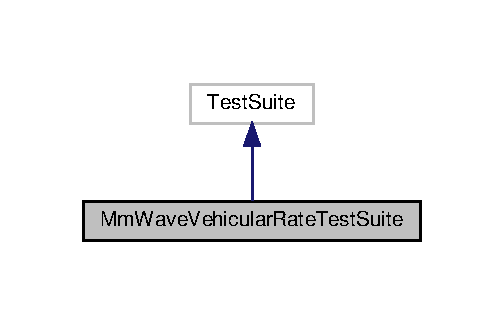
\includegraphics[width=242pt]{classMmWaveVehicularRateTestSuite__inherit__graph}
\end{center}
\end{figure}


Collaboration diagram for Mm\+Wave\+Vehicular\+Rate\+Test\+Suite\+:
\nopagebreak
\begin{figure}[H]
\begin{center}
\leavevmode
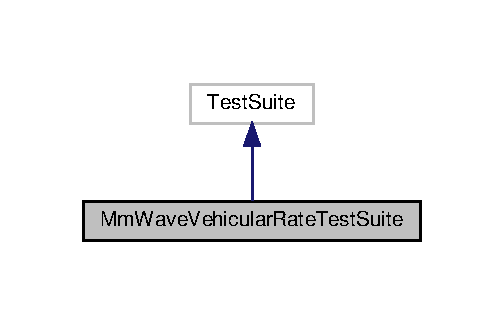
\includegraphics[width=242pt]{classMmWaveVehicularRateTestSuite__coll__graph}
\end{center}
\end{figure}


\subsection{Detailed Description}
Test suite for the class Mm\+Wave\+Sidelink\+Spectrum\+Phy 

The documentation for this class was generated from the following file\+:\begin{DoxyCompactItemize}
\item 
test/mmwave-\/vehicular-\/rate-\/test.\+cc\end{DoxyCompactItemize}

\hypertarget{classMmWaveVehicularSpectrumPhyTestCase1}{}\section{Mm\+Wave\+Vehicular\+Spectrum\+Phy\+Test\+Case1 Class Reference}
\label{classMmWaveVehicularSpectrumPhyTestCase1}\index{Mm\+Wave\+Vehicular\+Spectrum\+Phy\+Test\+Case1@{Mm\+Wave\+Vehicular\+Spectrum\+Phy\+Test\+Case1}}


Inheritance diagram for Mm\+Wave\+Vehicular\+Spectrum\+Phy\+Test\+Case1\+:\nopagebreak
\begin{figure}[H]
\begin{center}
\leavevmode
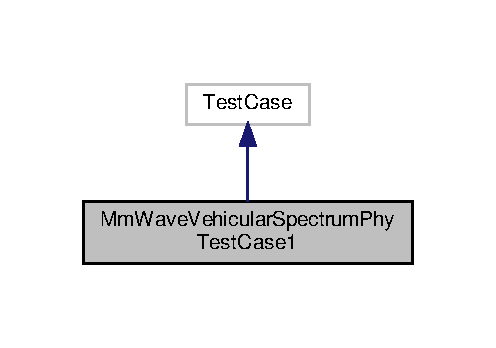
\includegraphics[width=238pt]{classMmWaveVehicularSpectrumPhyTestCase1__inherit__graph}
\end{center}
\end{figure}


Collaboration diagram for Mm\+Wave\+Vehicular\+Spectrum\+Phy\+Test\+Case1\+:\nopagebreak
\begin{figure}[H]
\begin{center}
\leavevmode
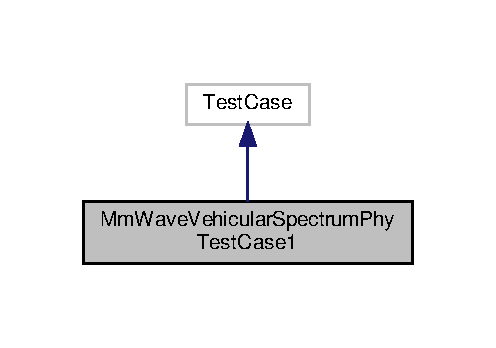
\includegraphics[width=238pt]{classMmWaveVehicularSpectrumPhyTestCase1__coll__graph}
\end{center}
\end{figure}
\subsection*{Public Member Functions}
\begin{DoxyCompactItemize}
\item 
\hyperlink{classMmWaveVehicularSpectrumPhyTestCase1_acbe3f1ab9c9eb3aa37dc8501240df04a}{Mm\+Wave\+Vehicular\+Spectrum\+Phy\+Test\+Case1} ()
\item 
virtual \hyperlink{classMmWaveVehicularSpectrumPhyTestCase1_a4317647a74efd1008350f294484eab1b}{$\sim$\+Mm\+Wave\+Vehicular\+Spectrum\+Phy\+Test\+Case1} ()
\end{DoxyCompactItemize}


\subsection{Detailed Description}
This is a test to check if the class Mm\+Wave\+Sidelink\+Spectrum\+Phy correctly computes the S\+NR. 

\subsection{Constructor \& Destructor Documentation}
\mbox{\Hypertarget{classMmWaveVehicularSpectrumPhyTestCase1_acbe3f1ab9c9eb3aa37dc8501240df04a}\label{classMmWaveVehicularSpectrumPhyTestCase1_acbe3f1ab9c9eb3aa37dc8501240df04a}} 
\index{Mm\+Wave\+Vehicular\+Spectrum\+Phy\+Test\+Case1@{Mm\+Wave\+Vehicular\+Spectrum\+Phy\+Test\+Case1}!Mm\+Wave\+Vehicular\+Spectrum\+Phy\+Test\+Case1@{Mm\+Wave\+Vehicular\+Spectrum\+Phy\+Test\+Case1}}
\index{Mm\+Wave\+Vehicular\+Spectrum\+Phy\+Test\+Case1@{Mm\+Wave\+Vehicular\+Spectrum\+Phy\+Test\+Case1}!Mm\+Wave\+Vehicular\+Spectrum\+Phy\+Test\+Case1@{Mm\+Wave\+Vehicular\+Spectrum\+Phy\+Test\+Case1}}
\subsubsection{\texorpdfstring{Mm\+Wave\+Vehicular\+Spectrum\+Phy\+Test\+Case1()}{MmWaveVehicularSpectrumPhyTestCase1()}}
{\footnotesize\ttfamily Mm\+Wave\+Vehicular\+Spectrum\+Phy\+Test\+Case1\+::\+Mm\+Wave\+Vehicular\+Spectrum\+Phy\+Test\+Case1 (\begin{DoxyParamCaption}{ }\end{DoxyParamCaption})}

Constructor \mbox{\Hypertarget{classMmWaveVehicularSpectrumPhyTestCase1_a4317647a74efd1008350f294484eab1b}\label{classMmWaveVehicularSpectrumPhyTestCase1_a4317647a74efd1008350f294484eab1b}} 
\index{Mm\+Wave\+Vehicular\+Spectrum\+Phy\+Test\+Case1@{Mm\+Wave\+Vehicular\+Spectrum\+Phy\+Test\+Case1}!````~Mm\+Wave\+Vehicular\+Spectrum\+Phy\+Test\+Case1@{$\sim$\+Mm\+Wave\+Vehicular\+Spectrum\+Phy\+Test\+Case1}}
\index{````~Mm\+Wave\+Vehicular\+Spectrum\+Phy\+Test\+Case1@{$\sim$\+Mm\+Wave\+Vehicular\+Spectrum\+Phy\+Test\+Case1}!Mm\+Wave\+Vehicular\+Spectrum\+Phy\+Test\+Case1@{Mm\+Wave\+Vehicular\+Spectrum\+Phy\+Test\+Case1}}
\subsubsection{\texorpdfstring{$\sim$\+Mm\+Wave\+Vehicular\+Spectrum\+Phy\+Test\+Case1()}{~MmWaveVehicularSpectrumPhyTestCase1()}}
{\footnotesize\ttfamily Mm\+Wave\+Vehicular\+Spectrum\+Phy\+Test\+Case1\+::$\sim$\+Mm\+Wave\+Vehicular\+Spectrum\+Phy\+Test\+Case1 (\begin{DoxyParamCaption}{ }\end{DoxyParamCaption})\hspace{0.3cm}{\ttfamily [virtual]}}

Destructor 

The documentation for this class was generated from the following file\+:\begin{DoxyCompactItemize}
\item 
test/mmwave-\/vehicular-\/spectrum-\/phy-\/test.\+cc\end{DoxyCompactItemize}

\hypertarget{classMmWaveVehicularSpectrumPhyTestSuite}{}\section{Mm\+Wave\+Vehicular\+Spectrum\+Phy\+Test\+Suite Class Reference}
\label{classMmWaveVehicularSpectrumPhyTestSuite}\index{Mm\+Wave\+Vehicular\+Spectrum\+Phy\+Test\+Suite@{Mm\+Wave\+Vehicular\+Spectrum\+Phy\+Test\+Suite}}


Inheritance diagram for Mm\+Wave\+Vehicular\+Spectrum\+Phy\+Test\+Suite\+:
\nopagebreak
\begin{figure}[H]
\begin{center}
\leavevmode
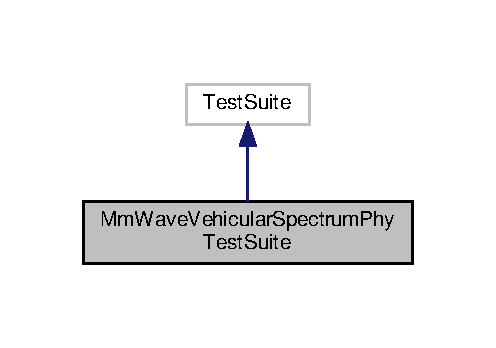
\includegraphics[width=238pt]{classMmWaveVehicularSpectrumPhyTestSuite__inherit__graph}
\end{center}
\end{figure}


Collaboration diagram for Mm\+Wave\+Vehicular\+Spectrum\+Phy\+Test\+Suite\+:
\nopagebreak
\begin{figure}[H]
\begin{center}
\leavevmode
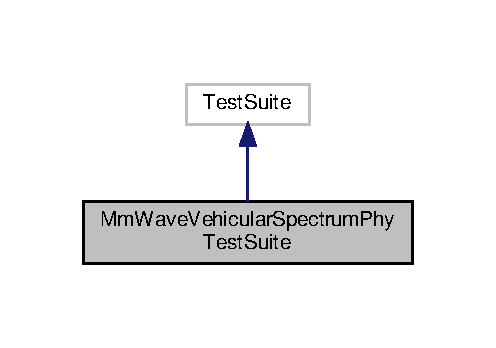
\includegraphics[width=238pt]{classMmWaveVehicularSpectrumPhyTestSuite__coll__graph}
\end{center}
\end{figure}


\subsection{Detailed Description}
Test suite for the class Mm\+Wave\+Sidelink\+Spectrum\+Phy 

The documentation for this class was generated from the following file\+:\begin{DoxyCompactItemize}
\item 
test/mmwave-\/vehicular-\/spectrum-\/phy-\/test.\+cc\end{DoxyCompactItemize}

\hypertarget{classns3_1_1millicar_1_1MmWaveVehicularSpectrumPropagationLossModel}{}\section{ns3\+:\+:millicar\+:\+:Mm\+Wave\+Vehicular\+Spectrum\+Propagation\+Loss\+Model Class Reference}
\label{classns3_1_1millicar_1_1MmWaveVehicularSpectrumPropagationLossModel}\index{ns3\+::millicar\+::\+Mm\+Wave\+Vehicular\+Spectrum\+Propagation\+Loss\+Model@{ns3\+::millicar\+::\+Mm\+Wave\+Vehicular\+Spectrum\+Propagation\+Loss\+Model}}


This class implements the fading computation of the 3\+G\+PP TR 38.\+900 channel model and performs the beamforming gain computation. It implements the Spectrum\+Propagation\+Loss\+Model interface.  




{\ttfamily \#include $<$mmwave-\/vehicular-\/spectrum-\/propagation-\/loss-\/model.\+h$>$}



Inheritance diagram for ns3\+:\+:millicar\+:\+:Mm\+Wave\+Vehicular\+Spectrum\+Propagation\+Loss\+Model\+:
\nopagebreak
\begin{figure}[H]
\begin{center}
\leavevmode
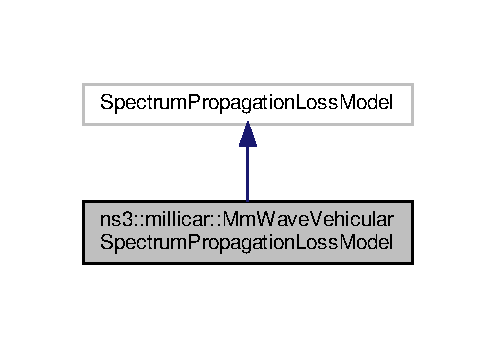
\includegraphics[width=238pt]{classns3_1_1millicar_1_1MmWaveVehicularSpectrumPropagationLossModel__inherit__graph}
\end{center}
\end{figure}


Collaboration diagram for ns3\+:\+:millicar\+:\+:Mm\+Wave\+Vehicular\+Spectrum\+Propagation\+Loss\+Model\+:
\nopagebreak
\begin{figure}[H]
\begin{center}
\leavevmode
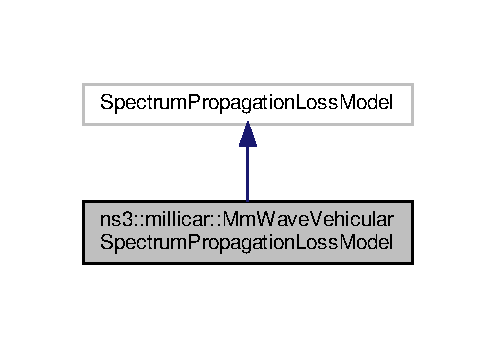
\includegraphics[width=238pt]{classns3_1_1millicar_1_1MmWaveVehicularSpectrumPropagationLossModel__coll__graph}
\end{center}
\end{figure}
\subsection*{Public Member Functions}
\begin{DoxyCompactItemize}
\item 
\hyperlink{classns3_1_1millicar_1_1MmWaveVehicularSpectrumPropagationLossModel_a9cb94e871be75a415ffd92015793a535}{Mm\+Wave\+Vehicular\+Spectrum\+Propagation\+Loss\+Model} ()
\item 
virtual \hyperlink{classns3_1_1millicar_1_1MmWaveVehicularSpectrumPropagationLossModel_aaa3809b4d4d0731f2206b71a0d5d9d9c}{$\sim$\+Mm\+Wave\+Vehicular\+Spectrum\+Propagation\+Loss\+Model} ()
\item 
\mbox{\Hypertarget{classns3_1_1millicar_1_1MmWaveVehicularSpectrumPropagationLossModel_a31388e68c063456d30daf210783b5f62}\label{classns3_1_1millicar_1_1MmWaveVehicularSpectrumPropagationLossModel_a31388e68c063456d30daf210783b5f62}} 
void {\bfseries Do\+Dispose} ()
\item 
void \hyperlink{classns3_1_1millicar_1_1MmWaveVehicularSpectrumPropagationLossModel_ab2c520f59106e0e7a919d6c724a8dd96}{Add\+Device} (Ptr$<$ Net\+Device $>$, Ptr$<$ \hyperlink{classns3_1_1millicar_1_1MmWaveVehicularAntennaArrayModel}{Mm\+Wave\+Vehicular\+Antenna\+Array\+Model} $>$)
\item 
void \hyperlink{classns3_1_1millicar_1_1MmWaveVehicularSpectrumPropagationLossModel_a87bc2bb292dc183649be9046062f3648}{Set\+Pathloss\+Model} (Ptr$<$ Propagation\+Loss\+Model $>$ pathloss)
\item 
void \hyperlink{classns3_1_1millicar_1_1MmWaveVehicularSpectrumPropagationLossModel_a0f59e8c2b0fa28ae37e2f239b6abaa1b}{Set\+Frequency} (double freq)
\item 
double \hyperlink{classns3_1_1millicar_1_1MmWaveVehicularSpectrumPropagationLossModel_ad9fb12c1bb96aa3bbd3eb676cdfa855f}{Get\+Frequency} (void) const
\end{DoxyCompactItemize}
\subsection*{Static Public Member Functions}
\begin{DoxyCompactItemize}
\item 
\mbox{\Hypertarget{classns3_1_1millicar_1_1MmWaveVehicularSpectrumPropagationLossModel_ae0e9dd0e9bf2c545e5673b18275b9321}\label{classns3_1_1millicar_1_1MmWaveVehicularSpectrumPropagationLossModel_ae0e9dd0e9bf2c545e5673b18275b9321}} 
static Type\+Id {\bfseries Get\+Type\+Id} (void)
\end{DoxyCompactItemize}


\subsection{Detailed Description}
This class implements the fading computation of the 3\+G\+PP TR 38.\+900 channel model and performs the beamforming gain computation. It implements the Spectrum\+Propagation\+Loss\+Model interface. 

\subsection{Constructor \& Destructor Documentation}
\mbox{\Hypertarget{classns3_1_1millicar_1_1MmWaveVehicularSpectrumPropagationLossModel_a9cb94e871be75a415ffd92015793a535}\label{classns3_1_1millicar_1_1MmWaveVehicularSpectrumPropagationLossModel_a9cb94e871be75a415ffd92015793a535}} 
\index{ns3\+::millicar\+::\+Mm\+Wave\+Vehicular\+Spectrum\+Propagation\+Loss\+Model@{ns3\+::millicar\+::\+Mm\+Wave\+Vehicular\+Spectrum\+Propagation\+Loss\+Model}!Mm\+Wave\+Vehicular\+Spectrum\+Propagation\+Loss\+Model@{Mm\+Wave\+Vehicular\+Spectrum\+Propagation\+Loss\+Model}}
\index{Mm\+Wave\+Vehicular\+Spectrum\+Propagation\+Loss\+Model@{Mm\+Wave\+Vehicular\+Spectrum\+Propagation\+Loss\+Model}!ns3\+::millicar\+::\+Mm\+Wave\+Vehicular\+Spectrum\+Propagation\+Loss\+Model@{ns3\+::millicar\+::\+Mm\+Wave\+Vehicular\+Spectrum\+Propagation\+Loss\+Model}}
\subsubsection{\texorpdfstring{Mm\+Wave\+Vehicular\+Spectrum\+Propagation\+Loss\+Model()}{MmWaveVehicularSpectrumPropagationLossModel()}}
{\footnotesize\ttfamily ns3\+::millicar\+::\+Mm\+Wave\+Vehicular\+Spectrum\+Propagation\+Loss\+Model\+::\+Mm\+Wave\+Vehicular\+Spectrum\+Propagation\+Loss\+Model (\begin{DoxyParamCaption}{ }\end{DoxyParamCaption})}

Constructor \mbox{\Hypertarget{classns3_1_1millicar_1_1MmWaveVehicularSpectrumPropagationLossModel_aaa3809b4d4d0731f2206b71a0d5d9d9c}\label{classns3_1_1millicar_1_1MmWaveVehicularSpectrumPropagationLossModel_aaa3809b4d4d0731f2206b71a0d5d9d9c}} 
\index{ns3\+::millicar\+::\+Mm\+Wave\+Vehicular\+Spectrum\+Propagation\+Loss\+Model@{ns3\+::millicar\+::\+Mm\+Wave\+Vehicular\+Spectrum\+Propagation\+Loss\+Model}!````~Mm\+Wave\+Vehicular\+Spectrum\+Propagation\+Loss\+Model@{$\sim$\+Mm\+Wave\+Vehicular\+Spectrum\+Propagation\+Loss\+Model}}
\index{````~Mm\+Wave\+Vehicular\+Spectrum\+Propagation\+Loss\+Model@{$\sim$\+Mm\+Wave\+Vehicular\+Spectrum\+Propagation\+Loss\+Model}!ns3\+::millicar\+::\+Mm\+Wave\+Vehicular\+Spectrum\+Propagation\+Loss\+Model@{ns3\+::millicar\+::\+Mm\+Wave\+Vehicular\+Spectrum\+Propagation\+Loss\+Model}}
\subsubsection{\texorpdfstring{$\sim$\+Mm\+Wave\+Vehicular\+Spectrum\+Propagation\+Loss\+Model()}{~MmWaveVehicularSpectrumPropagationLossModel()}}
{\footnotesize\ttfamily ns3\+::millicar\+::\+Mm\+Wave\+Vehicular\+Spectrum\+Propagation\+Loss\+Model\+::$\sim$\+Mm\+Wave\+Vehicular\+Spectrum\+Propagation\+Loss\+Model (\begin{DoxyParamCaption}{ }\end{DoxyParamCaption})\hspace{0.3cm}{\ttfamily [virtual]}}

Destructor 

\subsection{Member Function Documentation}
\mbox{\Hypertarget{classns3_1_1millicar_1_1MmWaveVehicularSpectrumPropagationLossModel_ab2c520f59106e0e7a919d6c724a8dd96}\label{classns3_1_1millicar_1_1MmWaveVehicularSpectrumPropagationLossModel_ab2c520f59106e0e7a919d6c724a8dd96}} 
\index{ns3\+::millicar\+::\+Mm\+Wave\+Vehicular\+Spectrum\+Propagation\+Loss\+Model@{ns3\+::millicar\+::\+Mm\+Wave\+Vehicular\+Spectrum\+Propagation\+Loss\+Model}!Add\+Device@{Add\+Device}}
\index{Add\+Device@{Add\+Device}!ns3\+::millicar\+::\+Mm\+Wave\+Vehicular\+Spectrum\+Propagation\+Loss\+Model@{ns3\+::millicar\+::\+Mm\+Wave\+Vehicular\+Spectrum\+Propagation\+Loss\+Model}}
\subsubsection{\texorpdfstring{Add\+Device()}{AddDevice()}}
{\footnotesize\ttfamily void ns3\+::millicar\+::\+Mm\+Wave\+Vehicular\+Spectrum\+Propagation\+Loss\+Model\+::\+Add\+Device (\begin{DoxyParamCaption}\item[{Ptr$<$ Net\+Device $>$}]{dev,  }\item[{Ptr$<$ \hyperlink{classns3_1_1millicar_1_1MmWaveVehicularAntennaArrayModel}{Mm\+Wave\+Vehicular\+Antenna\+Array\+Model} $>$}]{antenna }\end{DoxyParamCaption})}

Add a device 
\begin{DoxyParams}{Parameters}
{\em a} & pointer to the Net\+Device \\
\hline
{\em a} & pointer to the associated \hyperlink{classns3_1_1millicar_1_1MmWaveVehicularAntennaArrayModel}{Mm\+Wave\+Vehicular\+Antenna\+Array\+Model} \\
\hline
\end{DoxyParams}
\mbox{\Hypertarget{classns3_1_1millicar_1_1MmWaveVehicularSpectrumPropagationLossModel_ad9fb12c1bb96aa3bbd3eb676cdfa855f}\label{classns3_1_1millicar_1_1MmWaveVehicularSpectrumPropagationLossModel_ad9fb12c1bb96aa3bbd3eb676cdfa855f}} 
\index{ns3\+::millicar\+::\+Mm\+Wave\+Vehicular\+Spectrum\+Propagation\+Loss\+Model@{ns3\+::millicar\+::\+Mm\+Wave\+Vehicular\+Spectrum\+Propagation\+Loss\+Model}!Get\+Frequency@{Get\+Frequency}}
\index{Get\+Frequency@{Get\+Frequency}!ns3\+::millicar\+::\+Mm\+Wave\+Vehicular\+Spectrum\+Propagation\+Loss\+Model@{ns3\+::millicar\+::\+Mm\+Wave\+Vehicular\+Spectrum\+Propagation\+Loss\+Model}}
\subsubsection{\texorpdfstring{Get\+Frequency()}{GetFrequency()}}
{\footnotesize\ttfamily double ns3\+::millicar\+::\+Mm\+Wave\+Vehicular\+Spectrum\+Propagation\+Loss\+Model\+::\+Get\+Frequency (\begin{DoxyParamCaption}\item[{void}]{ }\end{DoxyParamCaption}) const}

\begin{DoxyReturn}{Returns}
the current frequency (Hz) 
\end{DoxyReturn}
\mbox{\Hypertarget{classns3_1_1millicar_1_1MmWaveVehicularSpectrumPropagationLossModel_a0f59e8c2b0fa28ae37e2f239b6abaa1b}\label{classns3_1_1millicar_1_1MmWaveVehicularSpectrumPropagationLossModel_a0f59e8c2b0fa28ae37e2f239b6abaa1b}} 
\index{ns3\+::millicar\+::\+Mm\+Wave\+Vehicular\+Spectrum\+Propagation\+Loss\+Model@{ns3\+::millicar\+::\+Mm\+Wave\+Vehicular\+Spectrum\+Propagation\+Loss\+Model}!Set\+Frequency@{Set\+Frequency}}
\index{Set\+Frequency@{Set\+Frequency}!ns3\+::millicar\+::\+Mm\+Wave\+Vehicular\+Spectrum\+Propagation\+Loss\+Model@{ns3\+::millicar\+::\+Mm\+Wave\+Vehicular\+Spectrum\+Propagation\+Loss\+Model}}
\subsubsection{\texorpdfstring{Set\+Frequency()}{SetFrequency()}}
{\footnotesize\ttfamily void ns3\+::millicar\+::\+Mm\+Wave\+Vehicular\+Spectrum\+Propagation\+Loss\+Model\+::\+Set\+Frequency (\begin{DoxyParamCaption}\item[{double}]{freq }\end{DoxyParamCaption})}


\begin{DoxyParams}{Parameters}
{\em freq} & the operating frequency (Hz) \\
\hline
\end{DoxyParams}
\mbox{\Hypertarget{classns3_1_1millicar_1_1MmWaveVehicularSpectrumPropagationLossModel_a87bc2bb292dc183649be9046062f3648}\label{classns3_1_1millicar_1_1MmWaveVehicularSpectrumPropagationLossModel_a87bc2bb292dc183649be9046062f3648}} 
\index{ns3\+::millicar\+::\+Mm\+Wave\+Vehicular\+Spectrum\+Propagation\+Loss\+Model@{ns3\+::millicar\+::\+Mm\+Wave\+Vehicular\+Spectrum\+Propagation\+Loss\+Model}!Set\+Pathloss\+Model@{Set\+Pathloss\+Model}}
\index{Set\+Pathloss\+Model@{Set\+Pathloss\+Model}!ns3\+::millicar\+::\+Mm\+Wave\+Vehicular\+Spectrum\+Propagation\+Loss\+Model@{ns3\+::millicar\+::\+Mm\+Wave\+Vehicular\+Spectrum\+Propagation\+Loss\+Model}}
\subsubsection{\texorpdfstring{Set\+Pathloss\+Model()}{SetPathlossModel()}}
{\footnotesize\ttfamily void ns3\+::millicar\+::\+Mm\+Wave\+Vehicular\+Spectrum\+Propagation\+Loss\+Model\+::\+Set\+Pathloss\+Model (\begin{DoxyParamCaption}\item[{Ptr$<$ Propagation\+Loss\+Model $>$}]{pathloss }\end{DoxyParamCaption})}

Set the pathloss model associated to this class 
\begin{DoxyParams}{Parameters}
{\em a} & pointer to the pathloss model, which has to implement the Propagation\+Loss\+Model interface \\
\hline
\end{DoxyParams}


The documentation for this class was generated from the following files\+:\begin{DoxyCompactItemize}
\item 
model/mmwave-\/vehicular-\/spectrum-\/propagation-\/loss-\/model.\+h\item 
model/mmwave-\/vehicular-\/spectrum-\/propagation-\/loss-\/model.\+cc\end{DoxyCompactItemize}

\hypertarget{classns3_1_1millicar_1_1MmWaveVehicularTracesHelper}{}\section{ns3\+:\+:millicar\+:\+:Mm\+Wave\+Vehicular\+Traces\+Helper Class Reference}
\label{classns3_1_1millicar_1_1MmWaveVehicularTracesHelper}\index{ns3\+::millicar\+::\+Mm\+Wave\+Vehicular\+Traces\+Helper@{ns3\+::millicar\+::\+Mm\+Wave\+Vehicular\+Traces\+Helper}}


{\ttfamily \#include $<$mmwave-\/vehicular-\/traces-\/helper.\+h$>$}



Inheritance diagram for ns3\+:\+:millicar\+:\+:Mm\+Wave\+Vehicular\+Traces\+Helper\+:
\nopagebreak
\begin{figure}[H]
\begin{center}
\leavevmode
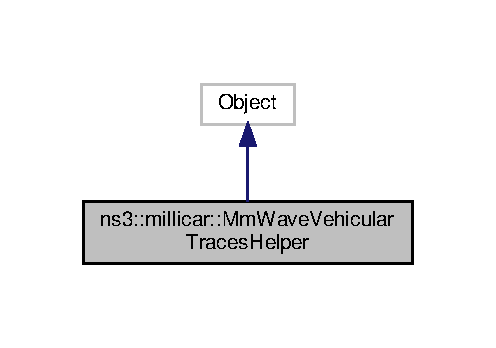
\includegraphics[width=238pt]{classns3_1_1millicar_1_1MmWaveVehicularTracesHelper__inherit__graph}
\end{center}
\end{figure}


Collaboration diagram for ns3\+:\+:millicar\+:\+:Mm\+Wave\+Vehicular\+Traces\+Helper\+:
\nopagebreak
\begin{figure}[H]
\begin{center}
\leavevmode
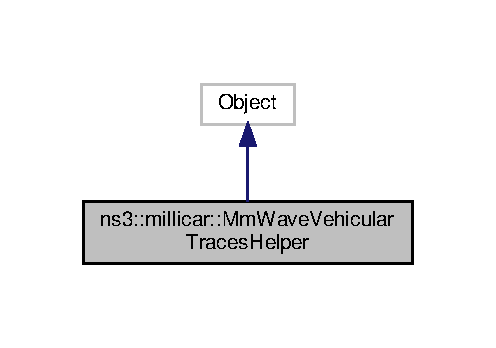
\includegraphics[width=238pt]{classns3_1_1millicar_1_1MmWaveVehicularTracesHelper__coll__graph}
\end{center}
\end{figure}
\subsection*{Public Member Functions}
\begin{DoxyCompactItemize}
\item 
\hyperlink{classns3_1_1millicar_1_1MmWaveVehicularTracesHelper_a097af2d4d714d26e5ed0f59f8ccaf9b7}{Mm\+Wave\+Vehicular\+Traces\+Helper} (std\+::string filename)
\item 
virtual \hyperlink{classns3_1_1millicar_1_1MmWaveVehicularTracesHelper_a55e4a6ddb57f316b089e8995e7647ef3}{$\sim$\+Mm\+Wave\+Vehicular\+Traces\+Helper} ()
\item 
void \hyperlink{classns3_1_1millicar_1_1MmWaveVehicularTracesHelper_a8f438f5c50ef9bf2c9dd10a9cb731845}{Mcs\+Sinr\+Callback} (const Spectrum\+Value \&sinr, uint16\+\_\+t rnti, uint8\+\_\+t num\+Sym, uint32\+\_\+t tb\+Size, uint8\+\_\+t mcs)
\end{DoxyCompactItemize}


\subsection{Detailed Description}
Class that manages the connection to a trace in \hyperlink{classns3_1_1millicar_1_1MmWaveSidelinkSpectrumPhy}{Mm\+Wave\+Sidelink\+Spectrum\+Phy} and prints to a file 

\subsection{Constructor \& Destructor Documentation}
\mbox{\Hypertarget{classns3_1_1millicar_1_1MmWaveVehicularTracesHelper_a097af2d4d714d26e5ed0f59f8ccaf9b7}\label{classns3_1_1millicar_1_1MmWaveVehicularTracesHelper_a097af2d4d714d26e5ed0f59f8ccaf9b7}} 
\index{ns3\+::millicar\+::\+Mm\+Wave\+Vehicular\+Traces\+Helper@{ns3\+::millicar\+::\+Mm\+Wave\+Vehicular\+Traces\+Helper}!Mm\+Wave\+Vehicular\+Traces\+Helper@{Mm\+Wave\+Vehicular\+Traces\+Helper}}
\index{Mm\+Wave\+Vehicular\+Traces\+Helper@{Mm\+Wave\+Vehicular\+Traces\+Helper}!ns3\+::millicar\+::\+Mm\+Wave\+Vehicular\+Traces\+Helper@{ns3\+::millicar\+::\+Mm\+Wave\+Vehicular\+Traces\+Helper}}
\subsubsection{\texorpdfstring{Mm\+Wave\+Vehicular\+Traces\+Helper()}{MmWaveVehicularTracesHelper()}}
{\footnotesize\ttfamily ns3\+::millicar\+::\+Mm\+Wave\+Vehicular\+Traces\+Helper\+::\+Mm\+Wave\+Vehicular\+Traces\+Helper (\begin{DoxyParamCaption}\item[{std\+::string}]{filename }\end{DoxyParamCaption})}

Constructor for this class 
\begin{DoxyParams}{Parameters}
{\em filename} & the name of the file \\
\hline
\end{DoxyParams}
\mbox{\Hypertarget{classns3_1_1millicar_1_1MmWaveVehicularTracesHelper_a55e4a6ddb57f316b089e8995e7647ef3}\label{classns3_1_1millicar_1_1MmWaveVehicularTracesHelper_a55e4a6ddb57f316b089e8995e7647ef3}} 
\index{ns3\+::millicar\+::\+Mm\+Wave\+Vehicular\+Traces\+Helper@{ns3\+::millicar\+::\+Mm\+Wave\+Vehicular\+Traces\+Helper}!````~Mm\+Wave\+Vehicular\+Traces\+Helper@{$\sim$\+Mm\+Wave\+Vehicular\+Traces\+Helper}}
\index{````~Mm\+Wave\+Vehicular\+Traces\+Helper@{$\sim$\+Mm\+Wave\+Vehicular\+Traces\+Helper}!ns3\+::millicar\+::\+Mm\+Wave\+Vehicular\+Traces\+Helper@{ns3\+::millicar\+::\+Mm\+Wave\+Vehicular\+Traces\+Helper}}
\subsubsection{\texorpdfstring{$\sim$\+Mm\+Wave\+Vehicular\+Traces\+Helper()}{~MmWaveVehicularTracesHelper()}}
{\footnotesize\ttfamily ns3\+::millicar\+::\+Mm\+Wave\+Vehicular\+Traces\+Helper\+::$\sim$\+Mm\+Wave\+Vehicular\+Traces\+Helper (\begin{DoxyParamCaption}{ }\end{DoxyParamCaption})\hspace{0.3cm}{\ttfamily [virtual]}}

Destructor for this class 

\subsection{Member Function Documentation}
\mbox{\Hypertarget{classns3_1_1millicar_1_1MmWaveVehicularTracesHelper_a8f438f5c50ef9bf2c9dd10a9cb731845}\label{classns3_1_1millicar_1_1MmWaveVehicularTracesHelper_a8f438f5c50ef9bf2c9dd10a9cb731845}} 
\index{ns3\+::millicar\+::\+Mm\+Wave\+Vehicular\+Traces\+Helper@{ns3\+::millicar\+::\+Mm\+Wave\+Vehicular\+Traces\+Helper}!Mcs\+Sinr\+Callback@{Mcs\+Sinr\+Callback}}
\index{Mcs\+Sinr\+Callback@{Mcs\+Sinr\+Callback}!ns3\+::millicar\+::\+Mm\+Wave\+Vehicular\+Traces\+Helper@{ns3\+::millicar\+::\+Mm\+Wave\+Vehicular\+Traces\+Helper}}
\subsubsection{\texorpdfstring{Mcs\+Sinr\+Callback()}{McsSinrCallback()}}
{\footnotesize\ttfamily void ns3\+::millicar\+::\+Mm\+Wave\+Vehicular\+Traces\+Helper\+::\+Mcs\+Sinr\+Callback (\begin{DoxyParamCaption}\item[{const Spectrum\+Value \&}]{sinr,  }\item[{uint16\+\_\+t}]{rnti,  }\item[{uint8\+\_\+t}]{num\+Sym,  }\item[{uint32\+\_\+t}]{tb\+Size,  }\item[{uint8\+\_\+t}]{mcs }\end{DoxyParamCaption})}

Method to be attached to the callback in the \hyperlink{classns3_1_1millicar_1_1MmWaveSidelinkSpectrumPhy}{Mm\+Wave\+Sidelink\+Spectrum\+Phy} 
\begin{DoxyParams}{Parameters}
{\em sinr} & pointer to the Spectrum\+Value instance representing the S\+I\+NR measured on all the spectrum chunks \\
\hline
{\em rnti} & the R\+N\+TI of the tranmitting device \\
\hline
{\em num\+Sym} & size of the transport block that generated the report in number of O\+F\+DM symbols \\
\hline
{\em tb\+Size} & size of the transport block that generated the report in bytes \\
\hline
{\em mcs} & the M\+CS of the transmission \\
\hline
\end{DoxyParams}


The documentation for this class was generated from the following files\+:\begin{DoxyCompactItemize}
\item 
helper/mmwave-\/vehicular-\/traces-\/helper.\+h\item 
helper/mmwave-\/vehicular-\/traces-\/helper.\+cc\end{DoxyCompactItemize}

\hypertarget{structns3_1_1millicar_1_1Params3gpp}{}\section{ns3\+:\+:millicar\+:\+:Params3gpp Struct Reference}
\label{structns3_1_1millicar_1_1Params3gpp}\index{ns3\+::millicar\+::\+Params3gpp@{ns3\+::millicar\+::\+Params3gpp}}


{\ttfamily \#include $<$mmwave-\/vehicular-\/spectrum-\/propagation-\/loss-\/model.\+h$>$}



Inheritance diagram for ns3\+:\+:millicar\+:\+:Params3gpp\+:
\nopagebreak
\begin{figure}[H]
\begin{center}
\leavevmode
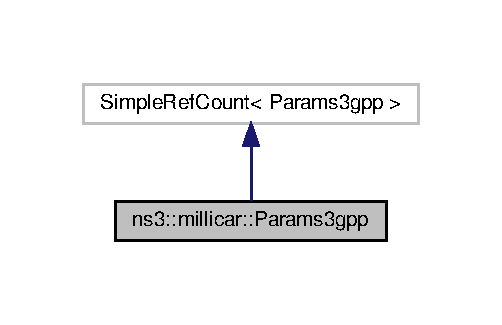
\includegraphics[width=241pt]{structns3_1_1millicar_1_1Params3gpp__inherit__graph}
\end{center}
\end{figure}


Collaboration diagram for ns3\+:\+:millicar\+:\+:Params3gpp\+:
\nopagebreak
\begin{figure}[H]
\begin{center}
\leavevmode
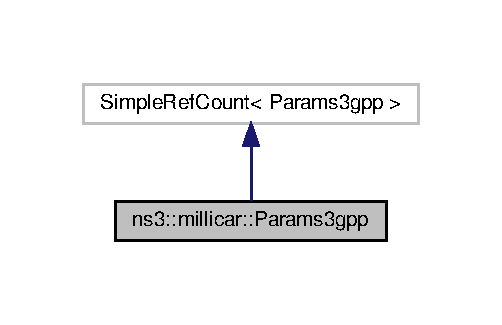
\includegraphics[width=241pt]{structns3_1_1millicar_1_1Params3gpp__coll__graph}
\end{center}
\end{figure}
\subsection*{Public Attributes}
\begin{DoxyCompactItemize}
\item 
\mbox{\Hypertarget{structns3_1_1millicar_1_1Params3gpp_aa672aff42743f756af3de779e2af4a05}\label{structns3_1_1millicar_1_1Params3gpp_aa672aff42743f756af3de779e2af4a05}} 
complex\+Vector\+\_\+t {\bfseries m\+\_\+txW}
\item 
\mbox{\Hypertarget{structns3_1_1millicar_1_1Params3gpp_a038c9030a2fb388d03646279804045e4}\label{structns3_1_1millicar_1_1Params3gpp_a038c9030a2fb388d03646279804045e4}} 
complex\+Vector\+\_\+t {\bfseries m\+\_\+rxW}
\item 
\mbox{\Hypertarget{structns3_1_1millicar_1_1Params3gpp_a9b81111656b981abbfe1ac21dfa74b63}\label{structns3_1_1millicar_1_1Params3gpp_a9b81111656b981abbfe1ac21dfa74b63}} 
complex3\+D\+Vector\+\_\+t {\bfseries m\+\_\+channel}
\item 
\mbox{\Hypertarget{structns3_1_1millicar_1_1Params3gpp_a5237e209e7d842da89f797136f80e0f1}\label{structns3_1_1millicar_1_1Params3gpp_a5237e209e7d842da89f797136f80e0f1}} 
double\+Vector\+\_\+t {\bfseries m\+\_\+delay}
\item 
\mbox{\Hypertarget{structns3_1_1millicar_1_1Params3gpp_a6ce25c8d9b9baacbdac0e9887b87e0fb}\label{structns3_1_1millicar_1_1Params3gpp_a6ce25c8d9b9baacbdac0e9887b87e0fb}} 
double {\bfseries m\+\_\+tau\+Delta}
\item 
\mbox{\Hypertarget{structns3_1_1millicar_1_1Params3gpp_a5d64ae0ddc01657a8032ea044f504d3f}\label{structns3_1_1millicar_1_1Params3gpp_a5d64ae0ddc01657a8032ea044f504d3f}} 
double2\+D\+Vector\+\_\+t {\bfseries m\+\_\+angle}
\item 
\mbox{\Hypertarget{structns3_1_1millicar_1_1Params3gpp_a933a29498ab43074972cd1cddf380f98}\label{structns3_1_1millicar_1_1Params3gpp_a933a29498ab43074972cd1cddf380f98}} 
complex\+Vector\+\_\+t {\bfseries m\+\_\+long\+Term}
\item 
\mbox{\Hypertarget{structns3_1_1millicar_1_1Params3gpp_a21d33af11e31ecc89ca22efc4b966e6c}\label{structns3_1_1millicar_1_1Params3gpp_a21d33af11e31ecc89ca22efc4b966e6c}} 
double2\+D\+Vector\+\_\+t {\bfseries m\+\_\+non\+Self\+Blocking}
\item 
\mbox{\Hypertarget{structns3_1_1millicar_1_1Params3gpp_ac237cf83dc199cda6b78cda843294ce5}\label{structns3_1_1millicar_1_1Params3gpp_ac237cf83dc199cda6b78cda843294ce5}} 
Vector {\bfseries m\+\_\+pre\+Loc\+UT}
\item 
\mbox{\Hypertarget{structns3_1_1millicar_1_1Params3gpp_a801d48451a22db6f9a60ef679fef6dfc}\label{structns3_1_1millicar_1_1Params3gpp_a801d48451a22db6f9a60ef679fef6dfc}} 
Vector {\bfseries m\+\_\+loc\+UT}
\item 
\mbox{\Hypertarget{structns3_1_1millicar_1_1Params3gpp_a8fc89b906602a260bd0ca96a29fd2a0d}\label{structns3_1_1millicar_1_1Params3gpp_a8fc89b906602a260bd0ca96a29fd2a0d}} 
double2\+D\+Vector\+\_\+t {\bfseries m\+\_\+nor\+Rv\+Angles}
\item 
\mbox{\Hypertarget{structns3_1_1millicar_1_1Params3gpp_a7203d21e53c36c311e1e4ea29a586ed9}\label{structns3_1_1millicar_1_1Params3gpp_a7203d21e53c36c311e1e4ea29a586ed9}} 
Time {\bfseries m\+\_\+generated\+Time}
\item 
\mbox{\Hypertarget{structns3_1_1millicar_1_1Params3gpp_a4b035a27176a2e5c7372610278bf2488}\label{structns3_1_1millicar_1_1Params3gpp_a4b035a27176a2e5c7372610278bf2488}} 
double {\bfseries m\+\_\+\+DS}
\item 
\mbox{\Hypertarget{structns3_1_1millicar_1_1Params3gpp_a2a98454b7730778cac396c2c4fbf0f5d}\label{structns3_1_1millicar_1_1Params3gpp_a2a98454b7730778cac396c2c4fbf0f5d}} 
double {\bfseries m\+\_\+K}
\item 
\mbox{\Hypertarget{structns3_1_1millicar_1_1Params3gpp_a899410f59c2adee760c17a262e696929}\label{structns3_1_1millicar_1_1Params3gpp_a899410f59c2adee760c17a262e696929}} 
uint8\+\_\+t {\bfseries m\+\_\+num\+Cluster}
\item 
\mbox{\Hypertarget{structns3_1_1millicar_1_1Params3gpp_a1f46df64fcee50c779ad55d720fa24fa}\label{structns3_1_1millicar_1_1Params3gpp_a1f46df64fcee50c779ad55d720fa24fa}} 
double2\+D\+Vector\+\_\+t {\bfseries m\+\_\+cluster\+Phase}
\item 
\mbox{\Hypertarget{structns3_1_1millicar_1_1Params3gpp_aa193c4d585689000b41e7bebaaf9674d}\label{structns3_1_1millicar_1_1Params3gpp_aa193c4d585689000b41e7bebaaf9674d}} 
double {\bfseries m\+\_\+los\+Phase}
\item 
\mbox{\Hypertarget{structns3_1_1millicar_1_1Params3gpp_afcf3e98c34a14297b2139c9418e78903}\label{structns3_1_1millicar_1_1Params3gpp_afcf3e98c34a14297b2139c9418e78903}} 
char {\bfseries m\+\_\+condition}
\item 
\mbox{\Hypertarget{structns3_1_1millicar_1_1Params3gpp_af78134fbc5a3bbc3bd0f7c305dfc33ea}\label{structns3_1_1millicar_1_1Params3gpp_af78134fbc5a3bbc3bd0f7c305dfc33ea}} 
bool {\bfseries m\+\_\+o2i}
\item 
\mbox{\Hypertarget{structns3_1_1millicar_1_1Params3gpp_a929cb38183705e922ab980df470baf5b}\label{structns3_1_1millicar_1_1Params3gpp_a929cb38183705e922ab980df470baf5b}} 
Vector {\bfseries m\+\_\+speed}
\item 
\mbox{\Hypertarget{structns3_1_1millicar_1_1Params3gpp_aff84718a12b5a5a6a946509b86308265}\label{structns3_1_1millicar_1_1Params3gpp_aff84718a12b5a5a6a946509b86308265}} 
double {\bfseries m\+\_\+dis2D}
\item 
\mbox{\Hypertarget{structns3_1_1millicar_1_1Params3gpp_abb16b534aee82802771ab2dd478f9a71}\label{structns3_1_1millicar_1_1Params3gpp_abb16b534aee82802771ab2dd478f9a71}} 
double {\bfseries m\+\_\+dis3D}
\item 
\mbox{\Hypertarget{structns3_1_1millicar_1_1Params3gpp_a4482c840103df226ec88d870475c2813}\label{structns3_1_1millicar_1_1Params3gpp_a4482c840103df226ec88d870475c2813}} 
std\+::map$<$ Ptr$<$ Net\+Device $>$, complex\+Vector\+\_\+t $>$ {\bfseries m\+\_\+all\+Long\+Term\+Map}
\end{DoxyCompactItemize}


\subsection{Detailed Description}
Data structure that stores a channel realization 

The documentation for this struct was generated from the following file\+:\begin{DoxyCompactItemize}
\item 
model/mmwave-\/vehicular-\/spectrum-\/propagation-\/loss-\/model.\+h\end{DoxyCompactItemize}

\hypertarget{structns3_1_1millicar_1_1ParamsTable}{}\section{ns3\+:\+:millicar\+:\+:Params\+Table Struct Reference}
\label{structns3_1_1millicar_1_1ParamsTable}\index{ns3\+::millicar\+::\+Params\+Table@{ns3\+::millicar\+::\+Params\+Table}}


{\ttfamily \#include $<$mmwave-\/vehicular-\/spectrum-\/propagation-\/loss-\/model.\+h$>$}



Inheritance diagram for ns3\+:\+:millicar\+:\+:Params\+Table\+:\nopagebreak
\begin{figure}[H]
\begin{center}
\leavevmode
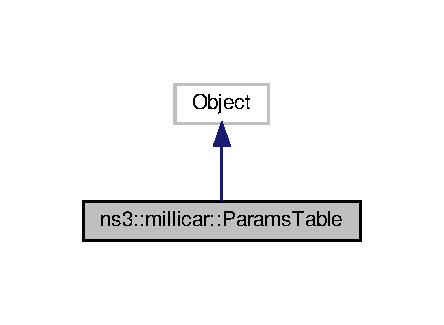
\includegraphics[width=213pt]{structns3_1_1millicar_1_1ParamsTable__inherit__graph}
\end{center}
\end{figure}


Collaboration diagram for ns3\+:\+:millicar\+:\+:Params\+Table\+:\nopagebreak
\begin{figure}[H]
\begin{center}
\leavevmode
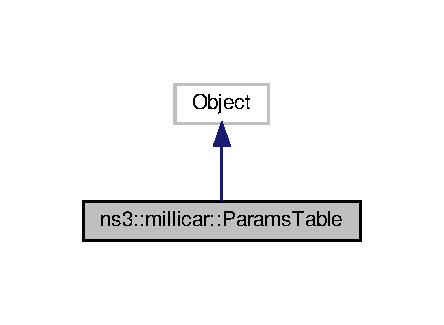
\includegraphics[width=213pt]{structns3_1_1millicar_1_1ParamsTable__coll__graph}
\end{center}
\end{figure}
\subsection*{Public Member Functions}
\begin{DoxyCompactItemize}
\item 
\mbox{\Hypertarget{structns3_1_1millicar_1_1ParamsTable_a530c30ffafcba89117eba9fb42c91f58}\label{structns3_1_1millicar_1_1ParamsTable_a530c30ffafcba89117eba9fb42c91f58}} 
void {\bfseries Set\+Params} (uint8\+\_\+t num\+Of\+Cluster, uint8\+\_\+t rays\+Per\+Cluster, double u\+Lg\+DS, double sig\+Lg\+DS, double u\+Lg\+A\+SD, double sig\+Lg\+A\+SD, double u\+Lg\+A\+SA, double sig\+Lg\+A\+SA, double u\+Lg\+Z\+SA, double sig\+Lg\+Z\+SA, double u\+Lg\+Z\+SD, double sig\+Lg\+Z\+SD, double offset\+Z\+OD, double c\+DS, double c\+A\+SD, double c\+A\+SA, double c\+Z\+SA, double uK, double sigK, double r\+Tau, double shadowing\+Std)
\end{DoxyCompactItemize}
\subsection*{Public Attributes}
\begin{DoxyCompactItemize}
\item 
\mbox{\Hypertarget{structns3_1_1millicar_1_1ParamsTable_ae1d4d1ee3e8170cc6f8f65aa12b6cbfb}\label{structns3_1_1millicar_1_1ParamsTable_ae1d4d1ee3e8170cc6f8f65aa12b6cbfb}} 
uint8\+\_\+t {\bfseries m\+\_\+num\+Of\+Cluster} = 0
\item 
\mbox{\Hypertarget{structns3_1_1millicar_1_1ParamsTable_aa8922cdc3faec15053ec6877521f6f7b}\label{structns3_1_1millicar_1_1ParamsTable_aa8922cdc3faec15053ec6877521f6f7b}} 
uint8\+\_\+t {\bfseries m\+\_\+rays\+Per\+Cluster} = 0
\item 
\mbox{\Hypertarget{structns3_1_1millicar_1_1ParamsTable_a684f5945b3da6252c6c710ddbe9e4b63}\label{structns3_1_1millicar_1_1ParamsTable_a684f5945b3da6252c6c710ddbe9e4b63}} 
double {\bfseries m\+\_\+u\+Lg\+DS} = 0
\item 
\mbox{\Hypertarget{structns3_1_1millicar_1_1ParamsTable_a1802ba8a755153b0ee57f042077930f4}\label{structns3_1_1millicar_1_1ParamsTable_a1802ba8a755153b0ee57f042077930f4}} 
double {\bfseries m\+\_\+sig\+Lg\+DS} = 0
\item 
\mbox{\Hypertarget{structns3_1_1millicar_1_1ParamsTable_abd231b80321b6d14c3313c0deebd5438}\label{structns3_1_1millicar_1_1ParamsTable_abd231b80321b6d14c3313c0deebd5438}} 
double {\bfseries m\+\_\+u\+Lg\+A\+SD} = 0
\item 
\mbox{\Hypertarget{structns3_1_1millicar_1_1ParamsTable_a7d6008f3854251ace7e554a7bdd0a733}\label{structns3_1_1millicar_1_1ParamsTable_a7d6008f3854251ace7e554a7bdd0a733}} 
double {\bfseries m\+\_\+sig\+Lg\+A\+SD} = 0
\item 
\mbox{\Hypertarget{structns3_1_1millicar_1_1ParamsTable_ab85d7c820732e853d66fb074cab526c4}\label{structns3_1_1millicar_1_1ParamsTable_ab85d7c820732e853d66fb074cab526c4}} 
double {\bfseries m\+\_\+u\+Lg\+A\+SA} = 0
\item 
\mbox{\Hypertarget{structns3_1_1millicar_1_1ParamsTable_ad8b3773ed38f423e15ad490c2448d9c1}\label{structns3_1_1millicar_1_1ParamsTable_ad8b3773ed38f423e15ad490c2448d9c1}} 
double {\bfseries m\+\_\+sig\+Lg\+A\+SA} = 0
\item 
\mbox{\Hypertarget{structns3_1_1millicar_1_1ParamsTable_ac2d5eb10c32e32b23a44378416b6a747}\label{structns3_1_1millicar_1_1ParamsTable_ac2d5eb10c32e32b23a44378416b6a747}} 
double {\bfseries m\+\_\+u\+Lg\+Z\+SA} = 0
\item 
\mbox{\Hypertarget{structns3_1_1millicar_1_1ParamsTable_a77bfbd263875c753541e91ee65e7a7e3}\label{structns3_1_1millicar_1_1ParamsTable_a77bfbd263875c753541e91ee65e7a7e3}} 
double {\bfseries m\+\_\+sig\+Lg\+Z\+SA} = 0
\item 
\mbox{\Hypertarget{structns3_1_1millicar_1_1ParamsTable_ae2b1cd3e760c51fd0a6e2c58ab6cfe56}\label{structns3_1_1millicar_1_1ParamsTable_ae2b1cd3e760c51fd0a6e2c58ab6cfe56}} 
double {\bfseries m\+\_\+u\+Lg\+Z\+SD} = 0
\item 
\mbox{\Hypertarget{structns3_1_1millicar_1_1ParamsTable_a31b09651d904e999d44c8c41992fbfd1}\label{structns3_1_1millicar_1_1ParamsTable_a31b09651d904e999d44c8c41992fbfd1}} 
double {\bfseries m\+\_\+sig\+Lg\+Z\+SD} = 0
\item 
\mbox{\Hypertarget{structns3_1_1millicar_1_1ParamsTable_a6b620d2150b7451f617db798de11cf02}\label{structns3_1_1millicar_1_1ParamsTable_a6b620d2150b7451f617db798de11cf02}} 
double {\bfseries m\+\_\+offset\+Z\+OD} = 0
\item 
\mbox{\Hypertarget{structns3_1_1millicar_1_1ParamsTable_a20a16108beb2fcc7500bf4422e8b775f}\label{structns3_1_1millicar_1_1ParamsTable_a20a16108beb2fcc7500bf4422e8b775f}} 
double {\bfseries m\+\_\+c\+DS} = 0
\item 
\mbox{\Hypertarget{structns3_1_1millicar_1_1ParamsTable_a27e9604955e0bac42e4a3a6b363e8cd0}\label{structns3_1_1millicar_1_1ParamsTable_a27e9604955e0bac42e4a3a6b363e8cd0}} 
double {\bfseries m\+\_\+c\+A\+SD} = 0
\item 
\mbox{\Hypertarget{structns3_1_1millicar_1_1ParamsTable_a4b366af107100981ce630cb8e9cea756}\label{structns3_1_1millicar_1_1ParamsTable_a4b366af107100981ce630cb8e9cea756}} 
double {\bfseries m\+\_\+c\+A\+SA} = 0
\item 
\mbox{\Hypertarget{structns3_1_1millicar_1_1ParamsTable_aa42795fc412a22da3338f911ba1c0790}\label{structns3_1_1millicar_1_1ParamsTable_aa42795fc412a22da3338f911ba1c0790}} 
double {\bfseries m\+\_\+c\+Z\+SA} = 0
\item 
\mbox{\Hypertarget{structns3_1_1millicar_1_1ParamsTable_a28f1d95964ed530448cc2f9954a2649d}\label{structns3_1_1millicar_1_1ParamsTable_a28f1d95964ed530448cc2f9954a2649d}} 
double {\bfseries m\+\_\+uK} = 0
\item 
\mbox{\Hypertarget{structns3_1_1millicar_1_1ParamsTable_a5825528eeaf7ca7657e5462c9b9e6558}\label{structns3_1_1millicar_1_1ParamsTable_a5825528eeaf7ca7657e5462c9b9e6558}} 
double {\bfseries m\+\_\+sigK} = 0
\item 
\mbox{\Hypertarget{structns3_1_1millicar_1_1ParamsTable_a69070ca57b3c78c2dd94712c3f6b32af}\label{structns3_1_1millicar_1_1ParamsTable_a69070ca57b3c78c2dd94712c3f6b32af}} 
double {\bfseries m\+\_\+r\+Tau} = 0
\item 
\mbox{\Hypertarget{structns3_1_1millicar_1_1ParamsTable_afefbe1da3cc2cad794d5812ba6023261}\label{structns3_1_1millicar_1_1ParamsTable_afefbe1da3cc2cad794d5812ba6023261}} 
double {\bfseries m\+\_\+shadowing\+Std} = 0
\item 
\mbox{\Hypertarget{structns3_1_1millicar_1_1ParamsTable_a49c997b83dfc2bedeea7a9971bc50f41}\label{structns3_1_1millicar_1_1ParamsTable_a49c997b83dfc2bedeea7a9971bc50f41}} 
double {\bfseries m\+\_\+sqrtC} \mbox{[}7\mbox{]}\mbox{[}7\mbox{]}
\end{DoxyCompactItemize}


\subsection{Detailed Description}
Data structure that stores the parameters of 3\+G\+PP TR 38.\+900, Table 7.\+5-\/6, for a certain scenario 

The documentation for this struct was generated from the following file\+:\begin{DoxyCompactItemize}
\item 
model/mmwave-\/vehicular-\/spectrum-\/propagation-\/loss-\/model.\+h\end{DoxyCompactItemize}

\hypertarget{classns3_1_1millicar_1_1PdcpSpecificSidelinkPdcpSapUser}{}\section{ns3\+:\+:millicar\+:\+:Pdcp\+Specific\+Sidelink\+Pdcp\+Sap\+User Class Reference}
\label{classns3_1_1millicar_1_1PdcpSpecificSidelinkPdcpSapUser}\index{ns3\+::millicar\+::\+Pdcp\+Specific\+Sidelink\+Pdcp\+Sap\+User@{ns3\+::millicar\+::\+Pdcp\+Specific\+Sidelink\+Pdcp\+Sap\+User}}


Inheritance diagram for ns3\+:\+:millicar\+:\+:Pdcp\+Specific\+Sidelink\+Pdcp\+Sap\+User\+:
\nopagebreak
\begin{figure}[H]
\begin{center}
\leavevmode
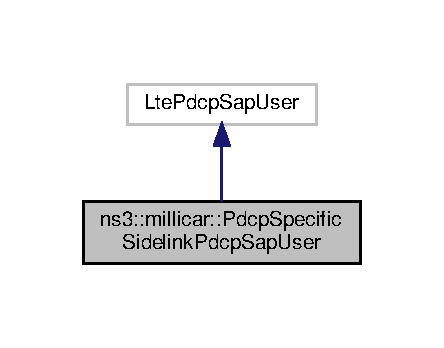
\includegraphics[width=213pt]{classns3_1_1millicar_1_1PdcpSpecificSidelinkPdcpSapUser__inherit__graph}
\end{center}
\end{figure}


Collaboration diagram for ns3\+:\+:millicar\+:\+:Pdcp\+Specific\+Sidelink\+Pdcp\+Sap\+User\+:
\nopagebreak
\begin{figure}[H]
\begin{center}
\leavevmode
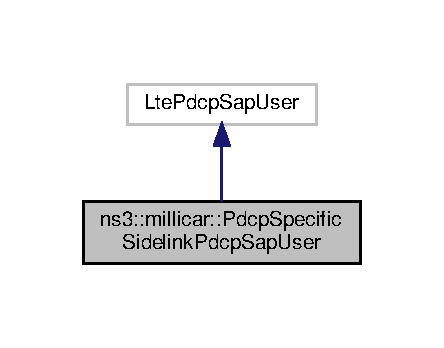
\includegraphics[width=213pt]{classns3_1_1millicar_1_1PdcpSpecificSidelinkPdcpSapUser__coll__graph}
\end{center}
\end{figure}
\subsection*{Public Member Functions}
\begin{DoxyCompactItemize}
\item 
\hyperlink{classns3_1_1millicar_1_1PdcpSpecificSidelinkPdcpSapUser_a010c7015eba9f2c373951760934ba8d9}{Pdcp\+Specific\+Sidelink\+Pdcp\+Sap\+User} (Ptr$<$ \hyperlink{classns3_1_1millicar_1_1MmWaveVehicularNetDevice}{Mm\+Wave\+Vehicular\+Net\+Device} $>$ net\+Device)
\item 
\mbox{\Hypertarget{classns3_1_1millicar_1_1PdcpSpecificSidelinkPdcpSapUser_a6ab83cbac459ceebae9434080d99b194}\label{classns3_1_1millicar_1_1PdcpSpecificSidelinkPdcpSapUser_a6ab83cbac459ceebae9434080d99b194}} 
virtual void {\bfseries Receive\+Pdcp\+Sdu} (Receive\+Pdcp\+Sdu\+Parameters params)
\end{DoxyCompactItemize}


\subsection{Constructor \& Destructor Documentation}
\mbox{\Hypertarget{classns3_1_1millicar_1_1PdcpSpecificSidelinkPdcpSapUser_a010c7015eba9f2c373951760934ba8d9}\label{classns3_1_1millicar_1_1PdcpSpecificSidelinkPdcpSapUser_a010c7015eba9f2c373951760934ba8d9}} 
\index{ns3\+::millicar\+::\+Pdcp\+Specific\+Sidelink\+Pdcp\+Sap\+User@{ns3\+::millicar\+::\+Pdcp\+Specific\+Sidelink\+Pdcp\+Sap\+User}!Pdcp\+Specific\+Sidelink\+Pdcp\+Sap\+User@{Pdcp\+Specific\+Sidelink\+Pdcp\+Sap\+User}}
\index{Pdcp\+Specific\+Sidelink\+Pdcp\+Sap\+User@{Pdcp\+Specific\+Sidelink\+Pdcp\+Sap\+User}!ns3\+::millicar\+::\+Pdcp\+Specific\+Sidelink\+Pdcp\+Sap\+User@{ns3\+::millicar\+::\+Pdcp\+Specific\+Sidelink\+Pdcp\+Sap\+User}}
\subsubsection{\texorpdfstring{Pdcp\+Specific\+Sidelink\+Pdcp\+Sap\+User()}{PdcpSpecificSidelinkPdcpSapUser()}}
{\footnotesize\ttfamily ns3\+::millicar\+::\+Pdcp\+Specific\+Sidelink\+Pdcp\+Sap\+User\+::\+Pdcp\+Specific\+Sidelink\+Pdcp\+Sap\+User (\begin{DoxyParamCaption}\item[{Ptr$<$ \hyperlink{classns3_1_1millicar_1_1MmWaveVehicularNetDevice}{Mm\+Wave\+Vehicular\+Net\+Device} $>$}]{net\+Device }\end{DoxyParamCaption})}

Constructor


\begin{DoxyParams}{Parameters}
{\em net\+Device} & the specific net\+Device to be connected to the P\+D\+CP S\+AP \\
\hline
\end{DoxyParams}


The documentation for this class was generated from the following files\+:\begin{DoxyCompactItemize}
\item 
model/mmwave-\/vehicular-\/net-\/device.\+h\item 
model/mmwave-\/vehicular-\/net-\/device.\+cc\end{DoxyCompactItemize}

\hypertarget{classns3_1_1millicar_1_1RlcSidelinkMemberMacSapProvider}{}\section{ns3\+:\+:millicar\+:\+:Rlc\+Sidelink\+Member\+Mac\+Sap\+Provider Class Reference}
\label{classns3_1_1millicar_1_1RlcSidelinkMemberMacSapProvider}\index{ns3\+::millicar\+::\+Rlc\+Sidelink\+Member\+Mac\+Sap\+Provider@{ns3\+::millicar\+::\+Rlc\+Sidelink\+Member\+Mac\+Sap\+Provider}}


Inheritance diagram for ns3\+:\+:millicar\+:\+:Rlc\+Sidelink\+Member\+Mac\+Sap\+Provider\+:\nopagebreak
\begin{figure}[H]
\begin{center}
\leavevmode
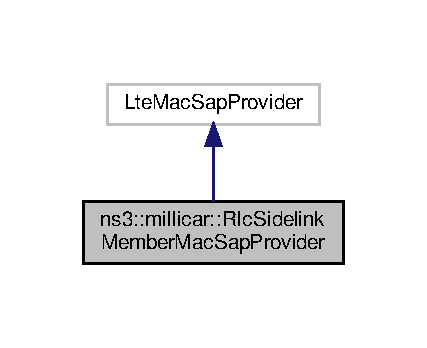
\includegraphics[width=205pt]{classns3_1_1millicar_1_1RlcSidelinkMemberMacSapProvider__inherit__graph}
\end{center}
\end{figure}


Collaboration diagram for ns3\+:\+:millicar\+:\+:Rlc\+Sidelink\+Member\+Mac\+Sap\+Provider\+:\nopagebreak
\begin{figure}[H]
\begin{center}
\leavevmode
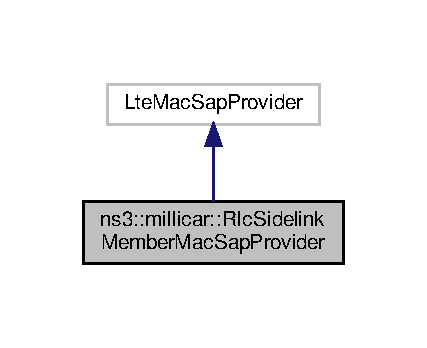
\includegraphics[width=205pt]{classns3_1_1millicar_1_1RlcSidelinkMemberMacSapProvider__coll__graph}
\end{center}
\end{figure}
\subsection*{Public Member Functions}
\begin{DoxyCompactItemize}
\item 
\hyperlink{classns3_1_1millicar_1_1RlcSidelinkMemberMacSapProvider_a178e79caf8df4d7bb738bb0dbef70530}{Rlc\+Sidelink\+Member\+Mac\+Sap\+Provider} (Ptr$<$ \hyperlink{classns3_1_1millicar_1_1MmWaveSidelinkMac}{Mm\+Wave\+Sidelink\+Mac} $>$ mac)
\item 
\mbox{\Hypertarget{classns3_1_1millicar_1_1RlcSidelinkMemberMacSapProvider_ae05a79a4fc56b618d90130ec39c9009d}\label{classns3_1_1millicar_1_1RlcSidelinkMemberMacSapProvider_ae05a79a4fc56b618d90130ec39c9009d}} 
virtual void {\bfseries Transmit\+Pdu} (Transmit\+Pdu\+Parameters params)
\item 
\mbox{\Hypertarget{classns3_1_1millicar_1_1RlcSidelinkMemberMacSapProvider_ac15e814e840c8b50cbfa7c60eef287dd}\label{classns3_1_1millicar_1_1RlcSidelinkMemberMacSapProvider_ac15e814e840c8b50cbfa7c60eef287dd}} 
virtual void {\bfseries Report\+Buffer\+Status} (Report\+Buffer\+Status\+Parameters params)
\end{DoxyCompactItemize}


\subsection{Constructor \& Destructor Documentation}
\mbox{\Hypertarget{classns3_1_1millicar_1_1RlcSidelinkMemberMacSapProvider_a178e79caf8df4d7bb738bb0dbef70530}\label{classns3_1_1millicar_1_1RlcSidelinkMemberMacSapProvider_a178e79caf8df4d7bb738bb0dbef70530}} 
\index{ns3\+::millicar\+::\+Rlc\+Sidelink\+Member\+Mac\+Sap\+Provider@{ns3\+::millicar\+::\+Rlc\+Sidelink\+Member\+Mac\+Sap\+Provider}!Rlc\+Sidelink\+Member\+Mac\+Sap\+Provider@{Rlc\+Sidelink\+Member\+Mac\+Sap\+Provider}}
\index{Rlc\+Sidelink\+Member\+Mac\+Sap\+Provider@{Rlc\+Sidelink\+Member\+Mac\+Sap\+Provider}!ns3\+::millicar\+::\+Rlc\+Sidelink\+Member\+Mac\+Sap\+Provider@{ns3\+::millicar\+::\+Rlc\+Sidelink\+Member\+Mac\+Sap\+Provider}}
\subsubsection{\texorpdfstring{Rlc\+Sidelink\+Member\+Mac\+Sap\+Provider()}{RlcSidelinkMemberMacSapProvider()}}
{\footnotesize\ttfamily ns3\+::millicar\+::\+Rlc\+Sidelink\+Member\+Mac\+Sap\+Provider\+::\+Rlc\+Sidelink\+Member\+Mac\+Sap\+Provider (\begin{DoxyParamCaption}\item[{Ptr$<$ \hyperlink{classns3_1_1millicar_1_1MmWaveSidelinkMac}{Mm\+Wave\+Sidelink\+Mac} $>$}]{mac }\end{DoxyParamCaption})}

Constructor


\begin{DoxyParams}{Parameters}
{\em mac} & the M\+AC class \\
\hline
\end{DoxyParams}


The documentation for this class was generated from the following files\+:\begin{DoxyCompactItemize}
\item 
model/mmwave-\/sidelink-\/mac.\+h\item 
model/mmwave-\/sidelink-\/mac.\+cc\end{DoxyCompactItemize}

\hypertarget{classns3_1_1millicar_1_1SidelinkRadioBearerInfo}{}\section{ns3\+:\+:millicar\+:\+:Sidelink\+Radio\+Bearer\+Info Class Reference}
\label{classns3_1_1millicar_1_1SidelinkRadioBearerInfo}\index{ns3\+::millicar\+::\+Sidelink\+Radio\+Bearer\+Info@{ns3\+::millicar\+::\+Sidelink\+Radio\+Bearer\+Info}}


{\ttfamily \#include $<$mmwave-\/vehicular-\/net-\/device.\+h$>$}



Inheritance diagram for ns3\+:\+:millicar\+:\+:Sidelink\+Radio\+Bearer\+Info\+:\nopagebreak
\begin{figure}[H]
\begin{center}
\leavevmode
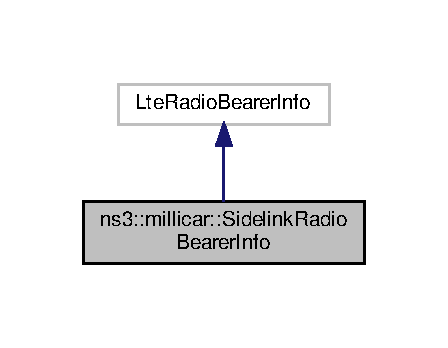
\includegraphics[width=215pt]{classns3_1_1millicar_1_1SidelinkRadioBearerInfo__inherit__graph}
\end{center}
\end{figure}


Collaboration diagram for ns3\+:\+:millicar\+:\+:Sidelink\+Radio\+Bearer\+Info\+:\nopagebreak
\begin{figure}[H]
\begin{center}
\leavevmode
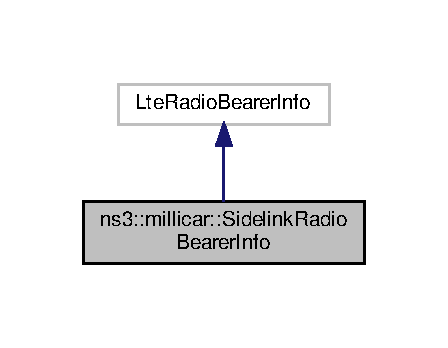
\includegraphics[width=215pt]{classns3_1_1millicar_1_1SidelinkRadioBearerInfo__coll__graph}
\end{center}
\end{figure}
\subsection*{Public Attributes}
\begin{DoxyCompactItemize}
\item 
\mbox{\Hypertarget{classns3_1_1millicar_1_1SidelinkRadioBearerInfo_abd89f4fdb332653516aec86da0d4e7c5}\label{classns3_1_1millicar_1_1SidelinkRadioBearerInfo_abd89f4fdb332653516aec86da0d4e7c5}} 
uint16\+\_\+t \hyperlink{classns3_1_1millicar_1_1SidelinkRadioBearerInfo_abd89f4fdb332653516aec86da0d4e7c5}{m\+\_\+rnti}
\begin{DoxyCompactList}\small\item\em rnti of the other endpoint of this bearer \end{DoxyCompactList}\end{DoxyCompactItemize}


\subsection{Detailed Description}
store information on active radio bearer instance 

The documentation for this class was generated from the following file\+:\begin{DoxyCompactItemize}
\item 
model/mmwave-\/vehicular-\/net-\/device.\+h\end{DoxyCompactItemize}

\hypertarget{structns3_1_1millicar_1_1SlSchedulingCallback}{}\section{ns3\+:\+:millicar\+:\+:Sl\+Scheduling\+Callback Struct Reference}
\label{structns3_1_1millicar_1_1SlSchedulingCallback}\index{ns3\+::millicar\+::\+Sl\+Scheduling\+Callback@{ns3\+::millicar\+::\+Sl\+Scheduling\+Callback}}


structure used for the scheduling info callback  




{\ttfamily \#include $<$mmwave-\/sidelink-\/mac.\+h$>$}

\subsection*{Public Attributes}
\begin{DoxyCompactItemize}
\item 
\mbox{\Hypertarget{structns3_1_1millicar_1_1SlSchedulingCallback_a1831e165e5378c4dc2e066795ff74028}\label{structns3_1_1millicar_1_1SlSchedulingCallback_a1831e165e5378c4dc2e066795ff74028}} 
uint16\+\_\+t \hyperlink{structns3_1_1millicar_1_1SlSchedulingCallback_a1831e165e5378c4dc2e066795ff74028}{frame}
\begin{DoxyCompactList}\small\item\em frame number \end{DoxyCompactList}\item 
\mbox{\Hypertarget{structns3_1_1millicar_1_1SlSchedulingCallback_a2acac5daa2ebddd899fe9710eb37c236}\label{structns3_1_1millicar_1_1SlSchedulingCallback_a2acac5daa2ebddd899fe9710eb37c236}} 
uint8\+\_\+t \hyperlink{structns3_1_1millicar_1_1SlSchedulingCallback_a2acac5daa2ebddd899fe9710eb37c236}{subframe}
\begin{DoxyCompactList}\small\item\em subframe number \end{DoxyCompactList}\item 
\mbox{\Hypertarget{structns3_1_1millicar_1_1SlSchedulingCallback_ae9162a29fa9912872f27bd9a5045e957}\label{structns3_1_1millicar_1_1SlSchedulingCallback_ae9162a29fa9912872f27bd9a5045e957}} 
uint8\+\_\+t \hyperlink{structns3_1_1millicar_1_1SlSchedulingCallback_ae9162a29fa9912872f27bd9a5045e957}{slot\+Num}
\begin{DoxyCompactList}\small\item\em slot number \end{DoxyCompactList}\item 
\mbox{\Hypertarget{structns3_1_1millicar_1_1SlSchedulingCallback_a94e0908bfa763bb1995a24bc855efb2a}\label{structns3_1_1millicar_1_1SlSchedulingCallback_a94e0908bfa763bb1995a24bc855efb2a}} 
uint8\+\_\+t \hyperlink{structns3_1_1millicar_1_1SlSchedulingCallback_a94e0908bfa763bb1995a24bc855efb2a}{sym\+Start}
\begin{DoxyCompactList}\small\item\em index of the starting symbol \end{DoxyCompactList}\item 
\mbox{\Hypertarget{structns3_1_1millicar_1_1SlSchedulingCallback_aeba85dc92c38c749b32d241abc30484d}\label{structns3_1_1millicar_1_1SlSchedulingCallback_aeba85dc92c38c749b32d241abc30484d}} 
uint8\+\_\+t \hyperlink{structns3_1_1millicar_1_1SlSchedulingCallback_aeba85dc92c38c749b32d241abc30484d}{num\+Sym}
\begin{DoxyCompactList}\small\item\em nummber of allocated symbols \end{DoxyCompactList}\item 
\mbox{\Hypertarget{structns3_1_1millicar_1_1SlSchedulingCallback_a1508f2b45509925dda62e706223dd3f5}\label{structns3_1_1millicar_1_1SlSchedulingCallback_a1508f2b45509925dda62e706223dd3f5}} 
uint8\+\_\+t \hyperlink{structns3_1_1millicar_1_1SlSchedulingCallback_a1508f2b45509925dda62e706223dd3f5}{mcs}
\begin{DoxyCompactList}\small\item\em the M\+CS for transport block \end{DoxyCompactList}\item 
\mbox{\Hypertarget{structns3_1_1millicar_1_1SlSchedulingCallback_a85afa95aa23c0a26f5526a198419bb3c}\label{structns3_1_1millicar_1_1SlSchedulingCallback_a85afa95aa23c0a26f5526a198419bb3c}} 
uint16\+\_\+t \hyperlink{structns3_1_1millicar_1_1SlSchedulingCallback_a85afa95aa23c0a26f5526a198419bb3c}{tb\+Size}
\begin{DoxyCompactList}\small\item\em the TB size in bytes \end{DoxyCompactList}\item 
\mbox{\Hypertarget{structns3_1_1millicar_1_1SlSchedulingCallback_adb434f6533e5a07eac34e2a12fd93dd7}\label{structns3_1_1millicar_1_1SlSchedulingCallback_adb434f6533e5a07eac34e2a12fd93dd7}} 
uint16\+\_\+t \hyperlink{structns3_1_1millicar_1_1SlSchedulingCallback_adb434f6533e5a07eac34e2a12fd93dd7}{tx\+Rnti}
\begin{DoxyCompactList}\small\item\em the R\+N\+TI which identifies the sender \end{DoxyCompactList}\item 
\mbox{\Hypertarget{structns3_1_1millicar_1_1SlSchedulingCallback_a68acb66f9d0cc3e2387436922f4c0c03}\label{structns3_1_1millicar_1_1SlSchedulingCallback_a68acb66f9d0cc3e2387436922f4c0c03}} 
uint16\+\_\+t \hyperlink{structns3_1_1millicar_1_1SlSchedulingCallback_a68acb66f9d0cc3e2387436922f4c0c03}{rx\+Rnti}
\begin{DoxyCompactList}\small\item\em the R\+N\+TI which identifies the destination \end{DoxyCompactList}\end{DoxyCompactItemize}


\subsection{Detailed Description}
structure used for the scheduling info callback 

The documentation for this struct was generated from the following file\+:\begin{DoxyCompactItemize}
\item 
model/mmwave-\/sidelink-\/mac.\+h\end{DoxyCompactItemize}

\hypertarget{structns3_1_1millicar_1_1TbInfo__t}{}\section{ns3\+:\+:millicar\+:\+:Tb\+Info\+\_\+t Struct Reference}
\label{structns3_1_1millicar_1_1TbInfo__t}\index{ns3\+::millicar\+::\+Tb\+Info\+\_\+t@{ns3\+::millicar\+::\+Tb\+Info\+\_\+t}}
\subsection*{Public Attributes}
\begin{DoxyCompactItemize}
\item 
\mbox{\Hypertarget{structns3_1_1millicar_1_1TbInfo__t_a5b908b8d39f67299cc7fb0a8fa49eaab}\label{structns3_1_1millicar_1_1TbInfo__t_a5b908b8d39f67299cc7fb0a8fa49eaab}} 
Ptr$<$ Packet\+Burst $>$ \hyperlink{structns3_1_1millicar_1_1TbInfo__t_a5b908b8d39f67299cc7fb0a8fa49eaab}{packet\+Burst}
\begin{DoxyCompactList}\small\item\em Packet burst associated to the transport block. \end{DoxyCompactList}\item 
\mbox{\Hypertarget{structns3_1_1millicar_1_1TbInfo__t_a7d2345dd012a4bd60660b2565184445b}\label{structns3_1_1millicar_1_1TbInfo__t_a7d2345dd012a4bd60660b2565184445b}} 
uint32\+\_\+t \hyperlink{structns3_1_1millicar_1_1TbInfo__t_a7d2345dd012a4bd60660b2565184445b}{size}
\begin{DoxyCompactList}\small\item\em Transport block size. \end{DoxyCompactList}\item 
\mbox{\Hypertarget{structns3_1_1millicar_1_1TbInfo__t_afa51577f7b4d9746d10252b4ba0a0e49}\label{structns3_1_1millicar_1_1TbInfo__t_afa51577f7b4d9746d10252b4ba0a0e49}} 
uint8\+\_\+t \hyperlink{structns3_1_1millicar_1_1TbInfo__t_afa51577f7b4d9746d10252b4ba0a0e49}{mcs}
\begin{DoxyCompactList}\small\item\em M\+CS. \end{DoxyCompactList}\item 
\mbox{\Hypertarget{structns3_1_1millicar_1_1TbInfo__t_a96d967f1f338fad94833ff303dc49748}\label{structns3_1_1millicar_1_1TbInfo__t_a96d967f1f338fad94833ff303dc49748}} 
uint8\+\_\+t \hyperlink{structns3_1_1millicar_1_1TbInfo__t_a96d967f1f338fad94833ff303dc49748}{num\+Sym}
\begin{DoxyCompactList}\small\item\em number of symbols used to transmit this TB \end{DoxyCompactList}\item 
\mbox{\Hypertarget{structns3_1_1millicar_1_1TbInfo__t_a81087edab29d0c02c7e23f1f9484fcdc}\label{structns3_1_1millicar_1_1TbInfo__t_a81087edab29d0c02c7e23f1f9484fcdc}} 
uint16\+\_\+t \hyperlink{structns3_1_1millicar_1_1TbInfo__t_a81087edab29d0c02c7e23f1f9484fcdc}{rnti}
\begin{DoxyCompactList}\small\item\em R\+N\+TI of the device which is sending the packet. \end{DoxyCompactList}\item 
\mbox{\Hypertarget{structns3_1_1millicar_1_1TbInfo__t_a4bb819dcf5cb940500997b5387012f4b}\label{structns3_1_1millicar_1_1TbInfo__t_a4bb819dcf5cb940500997b5387012f4b}} 
std\+::vector$<$ int $>$ \hyperlink{structns3_1_1millicar_1_1TbInfo__t_a4bb819dcf5cb940500997b5387012f4b}{rb\+Bitmap}
\begin{DoxyCompactList}\small\item\em Resource block bitmap. \end{DoxyCompactList}\end{DoxyCompactItemize}


The documentation for this struct was generated from the following file\+:\begin{DoxyCompactItemize}
\item 
model/mmwave-\/sidelink-\/spectrum-\/phy.\+h\end{DoxyCompactItemize}

%--- End generated contents ---

% Index
\backmatter
\newpage
\phantomsection
\clearemptydoublepage
\addcontentsline{toc}{chapter}{Index}
\printindex

\end{document}
